%%%%%%%%%%%%%%%%%%%%%%%%%%%%%%%%%%%%%%%%%%%%%%%%%%%%%%%%%%%%%%%%%%%%%%%%%
%
%   LaTeX File for Doctor (Master) Thesis of Tsinghua University
%   LaTeX + CJK     清华大学博士\KH{硕士}论文模板
%   Based on Wang Tianshu's Template for XJTU
%   Version: 1.00
%   Last Update: 2003-09-12
%
%%%%%%%%%%%%%%%%%%%%%%%%%%%%%%%%%%%%%%%%%%%%%%%%%%%%%%%%%%%%%%%%%%%%%%%%%
%   Copyright 2002-2003  by  Lei Wang (BaconChina)       (bcpub@sina.com)
%%%%%%%%%%%%%%%%%%%%%%%%%%%%%%%%%%%%%%%%%%%%%%%%%%%%%%%%%%%%%%%%%%%%%%%%%

%%%%%%%%%%%%%%%%%%%%%%%%%%%%%%%%%%%%%%%%%%%%%%%%%%%%%%%%%%%%%%%%%%%%%%%%%
%
%   LaTeX File for phd thesis of xi'an Jiao Tong University
%
%%%%%%%%%%%%%%%%%%%%%%%%%%%%%%%%%%%%%%%%%%%%%%%%%%%%%%%%%%%%%%%%%%%%%%%%%
%   Copyright 2002  by  Wang Tianshu    (tswang@asia.com)
%%%%%%%%%%%%%%%%%%%%%%%%%%%%%%%%%%%%%%%%%%%%%%%%%%%%%%%%%%%%%%%%%%%%%%%%%

%%%%%%%%%%%%%%%%%%%%%%%%%%%%%%%%%%%%%%%%%%%%%%%%%%%%%%%%%%%
%
% Latex 西安交通大学博士论文的模板.
%
% 建议使用miktex2.1最大安装编译此模板
%
%%%%%%%%%%%%%%%%%%%%%%%%%%%%%%%%%%%%%%%%%%%%%%%%%%%%%%%%%%


%draft 选项可以使插入的图形只显示外框,以加快预览速度。
%fleqn 让公式左对齐。
\documentclass[12pt,a4paper,openany,oneside]{book}
%\documentclass[11pt,a4paper,openany,draft]{book}
%\documentclass[11pt,a4paper,fleqn,openany,draft]{book}
%\documentclass[11pt,a4paper,fleqn,openany,draft]{book}

%以下是采用dvipdfmx所需设置
%\AtBeginDvi{\special{pdf:tounicode GBK-EUC-UCS2}}
%\usepackage[CJKbookmarks=true,dvipdfm,
%           hyperindex=true,
%           pdfstartview=FitH,
%           bookmarksnumbered=true,
%           bookmarksopen=true,
%           colorlinks=true, %注释掉此项则交叉引用为彩色边框(将colorlinks和pdfborder同时注释掉)
%           pdfborder=001,   %注释掉此项则交叉引用为彩色边框
%           citecolor=blue%
%           ]{hyperref}
%%%%%%%%%%%%%%%%%%%%%%%%%%%%%%%%%%%%%%%%%%%%%%%%%%%%%%%%%%%
%
% 引用的宏包
%
%%%%%%%%%%%%%%%%%%%%%%%%%%%%%%%%%%%%%%%%%%%%%%%%%%%%%%%%%%%

%%%%%%%%%%%%%%%%%%%%%%%%%%%%%%%%%%%%%%%%%%%%%%%%%%%%%%%%%%%%%%%%%%%%%%%%%
%
%   LaTeX File for Doctor (Master) Thesis of Tsinghua University
%   LaTeX + CJK     清华大学博士(硕士)论文模板
%   Based on Wang Tianshu's Template for XJTU
%	Version: 1.00
%   Last Update: 2003-09-12
%
%%%%%%%%%%%%%%%%%%%%%%%%%%%%%%%%%%%%%%%%%%%%%%%%%%%%%%%%%%%%%%%%%%%%%%%%%
%   Copyright 2002-2003  by  Lei Wang (BaconChina)       (bcpub@sina.com)
%%%%%%%%%%%%%%%%%%%%%%%%%%%%%%%%%%%%%%%%%%%%%%%%%%%%%%%%%%%%%%%%%%%%%%%%%

%%%%%%%%%%%%%%%%%%%%%%%%%%%%%%%%%%%%%%%%%%%%%%%%%%%%%%%%%%%%%%%%%%%%%%%%%
%
%   LaTeX File for phd thesis of xi'an Jiao Tong University
%
%%%%%%%%%%%%%%%%%%%%%%%%%%%%%%%%%%%%%%%%%%%%%%%%%%%%%%%%%%%%%%%%%%%%%%%%%
%   Copyright 2002  by  Wang Tianshu    (tswang@asia.com)
%%%%%%%%%%%%%%%%%%%%%%%%%%%%%%%%%%%%%%%%%%%%%%%%%%%%%%%%%%%%%%%%%%%%%%%%%

%%%%%%%%%%%%%%%%%%%%%%%%%%%%%%%%%%%%%%%%%%%%%%%%%%%%%%%%%%%
%
% 引用的宏包和相应的定义
%
%%%%%%%%%%%%%%%%%%%%%%%%%%%%%%%%%%%%%%%%%%%%%%%%%%%%%%%%%%%

\usepackage[dvips]{graphicx}
\usepackage{subfigure}
% 支持彩色
\usepackage{color}
% eps图像
\usepackage{epsfig}

%\else
%\usepackage[dvips]{graphicx}
%\usepackage{subfigure}
%\fi

% 首行缩进宏包
\usepackage{indentfirst}

% 版面控制宏包,定义规定的版面尺寸
\usepackage[top=1.0in,
        bottom=1.6in,
        left=1.2in,
        right=1.2in,
            %twosideshift=0 pt,
            %headheight=1.0true cm
            ]{geometry}

%\usepackage[top=4.0cm,
        %bottom=1.6in,
        %left=2.5cm,
        %right=2.5cm,
            %%twosideshift=0 pt,
            %%headheight=1.0true cm
            %]{geometry}

% 脚注控制
\usepackage[perpage,symbol]{footmisc}

% AMSLaTeX宏包 用来排出更加漂亮的公式
\usepackage{amsmath}
\usepackage{amssymb}

% 不同于\mathcal or \mathfrak 之类的英文花体字体
\usepackage{mathrsfs}

% 定理类环境宏包,其中 amsmath 选项用来兼容 AMS LaTeX 的宏包
\usepackage[amsmath,thmmarks]{ntheorem}

% 因为图形可浮动到当前页的顶部,所以它可能会出现
% 在它所在文本的前面. 要防止这种情况,可使用 flafter
% 宏包
%\usepackage{flafter}

%浮动图形控制宏包
%允许上一个section的浮动图形出现在下一个section的开始部分
%该宏包提供处理浮动对象的 \FloatBarrier 命令,使所有未处
%理的浮动图形立即被处理
\usepackage[below]{placeins}

% 图文混排用宏包
%\usepackage{floatflt}

% 图形和表格的控制
\usepackage{rotating}

% tex1cm宏包,控制字体的大小
\usepackage{type1cm}

% 控制标题的宏包
\usepackage[sf]{titlesec}

% 控制目录的宏包
\usepackage{titletoc}

% 处理数学公式中的黑斜体的宏包
\usepackage{bm}

%可将浮动对象放置到文件的最后
%\usepackage{endfloat}

% fancyhdr宏包 页眉和页脚的相关定义
\usepackage{fancyhdr}
\usepackage{fancyref}

% 支持引用的宏包
\usepackage{cite}

% Booktab
\usepackage{booktabs} % for much better looking tables

%浮动图形和表格标题样式
%\usepackage{caption2}
\usepackage[font=footnotesize]{caption}

% 定制表格和图形的多行标题行距
\usepackage{setspace}

% 打印当前页面格式的宏包
\usepackage{layouts}

% 使用Times字体的宏包
%\usepackage{times}

% qiuying add
\usepackage[BoldFont, SlantFont]{xeCJK}
\punctstyle{quanjiao}
\usepackage{tikz}
\usepackage{listings}

% 生成带书签的pdf
\usepackage[CJKbookmarks=true,
            bookmarksnumbered=true,
            bookmarksopen=true,
            colorlinks=true,
            pdfborder=001,
            citecolor=black,
            linkcolor=black,
            anchorcolor=green,
            urlcolor=black,
	  pdftitle={本科毕业设计论文},
	  pdfcreator={XeTeX,XeCJK},
	  pdfproducer={XeTeX},% 这个好像没起作用? 
            ]{hyperref}

\usepackage{enumitem}

\usepackage{float}

%\usepackage{ctexcap}

%%%%%%%%%%%%%%%%%%%%%%%%%%%%%%%%%%%%%%%%%%%%%%%%%%%%%%%%%%%%%%%%%%%%%%%%%
%
%   LaTeX File for Doctor (Master) Thesis of Tsinghua University
%   LaTeX + CJK     清华大学博士(硕士)论文模板
%   Based on Wang Tianshu's Template for XJTU
%   Version: 1.00
%   Last Update: 2003-09-12
%
%%%%%%%%%%%%%%%%%%%%%%%%%%%%%%%%%%%%%%%%%%%%%%%%%%%%%%%%%%%%%%%%%%%%%%%%%
%   Copyright 2002-2003  by  Lei Wang (BaconChina)       (bcpub@sina.com)
%%%%%%%%%%%%%%%%%%%%%%%%%%%%%%%%%%%%%%%%%%%%%%%%%%%%%%%%%%%%%%%%%%%%%%%%%

%%%%%%%%%%%%%%%%%%%%%%%%%%%%%%%%%%%%%%%%%%%%%%%%%%%%%%%%%%%%%%%%%%%%%%%%%
%
%   LaTeX File for phd thesis of xi'an Jiao Tong University
%
%%%%%%%%%%%%%%%%%%%%%%%%%%%%%%%%%%%%%%%%%%%%%%%%%%%%%%%%%%%%%%%%%%%%%%%%%
%   Copyright 2002  by  Wang Tianshu    (tswang@asia.com)
%%%%%%%%%%%%%%%%%%%%%%%%%%%%%%%%%%%%%%%%%%%%%%%%%%%%%%%%%%%%%%%%%%%%%%%%%
%%%%%%%%%%%%%%%%%%%%%%%%%%%%%%%%%%%%%%%%%%%%%%%%%%%%%%%%%%%
%
% 主文档 格式定义
%
%%%%%%%%%%%%%%%%%%%%%%%%%%%%%%%%%%%%%%%%%%%%%%%%%%%%%%%%%%%

% 按清华标准, 将版芯控制在240mm以内, 正文范围控制在220mm以内
%\addtolength{\headsep}{-0.1cm}          %页眉位置
%\addtolength{\footskip}{-0.1cm}         %页脚位置
\addtolength{\topmargin}{0.5cm}

%%%%%%%%%%%%%%%%%%%%%%%%%%%%%%%%%%%%%%%%%%%%%%%%%%%%%%%%%%%
% 公式的精调
%%%%%%%%%%%%%%%%%%%%%%%%%%%%%%%%%%%%%%%%%%%%%%%%%%%%%%%%%%%

%\setlength{\mathindent}{4.7 em}     %左对齐公式缩进量

% \eqnarray如果很长,影响分栏、换行和分页(整块挪动,造成页面空白),
% 可以设置成为自动调整模式
\allowdisplaybreaks[4]

%%%%%%%%%%%%%%%%%%%%%%%%%%%%%%%%%%%%%%%%%%%%%%%%%%%%%%%%%%%
%下面这组命令使浮动对象的缺省值稍微宽松一点,从而防止幅度
%对象占据过多的文本页面,也可以防止在很大空白的浮动页上放置
%很小的图形。
%%%%%%%%%%%%%%%%%%%%%%%%%%%%%%%%%%%%%%%%%%%%%%%%%%%%%%%%%%%
\renewcommand{\textfraction}{0.15}
\renewcommand{\topfraction}{0.85}
\renewcommand{\bottomfraction}{0.65}
\renewcommand{\floatpagefraction}{0.60}


%%%%%%%%%%%%%%%%%%%%%%%%%%%%%%%%%%%%%%%%%%%%%%%%%%%%%%%%%%%
%下面这组命令可以使公式编号随着每开始新的一节而重新开始。
%%%%%%%%%%%%%%%%%%%%%%%%%%%%%%%%%%%%%%%%%%%%%%%%%%%%%%%%%%%

%\makeatletter      % '@' is now a normail "letter" for TeX
%\@addtoreset{eqation}{section}
%\makeatother       % '@' is restored as a "non-letter" character for TeX

%%%%%%%%%%%%%%%%%%%%%%%%%%%%%%%%%%%%%%%%%%%%%%%%%%%%%%%%%%%
% 重定义字体命令
%%%%%%%%%%%%%%%%%%%%%%%%%%%%%%%%%%%%%%%%%%%%%%%%%%%%%%%%%%%
% 注意win2000,没有 simsun, 最好到网上找一个
% 一些字体是office2000 带的
%%%%%%%%%%%%%%%%%%%%%%%%%%%%%%%%%%%%%%%%%%%%%%%%%%%%%%%%%%%

%\setmainfont{TeX Gyre Termes}
%\setsansfont{TeX Gyre Heros}
%\setmonofont{TeX Gyre Cursor}
%\setCJKmainfont[BoldFont={方正小标宋简体}]{Adobe Song Std}    % 宋体  
%\setCJKsansfont{Adobe Heiti Std}
%\setCJKmonofont{Adobe Fangsong Std}
\setCJKmainfont[BoldFont=SimHei]{SimSun}    % 宋体  
\setCJKsansfont{SimHei}
%\setCJKmonofont{FangSong_GB2312}
\setCJKmonofont{FangSong}

%\setCJKfamilyfont{song}[BoldFont={方正宋黑简体}]{SimSun}      	% 宋体  
%\setCJKfamilyfont{song}[BoldFont={方正宋三_GBK}]{方正博雅宋_GBK}  % 宋体  
%\setCJKfamilyfont{song}[BoldFont={Adobe Heiti Std}]{Adobe Song Std}    % 宋体  
%\setCJKfamilyfont{song}[BoldFont={华文中宋}]{华文宋体}    % 宋体  
%\setCJKfamilyfont{song}[BoldFont={方正大标宋_GBK}]{方正兰亭宋_GBK}    % 宋体  
%\setCJKfamilyfont{song}[BoldFont={方正小标宋简体}]{方正书宋简体}    % 宋体  
%文泉驿微米黑
%\setCJKfamilyfont{song}[BoldFont={方正小标宋简体}]{Adobe Song Std}    % 宋体  
\setCJKfamilyfont{song}{SimSun}    			% 宋体  
\setCJKfamilyfont{hei}{SimHei}      		% 黑体  
%\setCJKfamilyfont{kai}{KaiTi_GB2312}      	% 楷体  
\setCJKfamilyfont{kai}{KaiTi}      	% 楷体  
\setCJKfamilyfont{fang}{Fangsong}  	% 仿宋体
%\setCJKfamilyfont{nwpulogo}{nwpulogo}     	% 含"西北工业大学"logo字体 
\setCJKfamilyfont{nwpulogo}{KaiTi}     	% 含"西北工业大学"logo字体 

\newcommand{\song}{\CJKfamily{song}}
\newcommand{\hei}{\CJKfamily{hei}}
\newcommand{\fang}{\CJKfamily{fang}}
\newcommand{\kai}{\CJKfamily{kai}}
\newcommand{\nwpulogo}{\CJKfamily{nwpulogo}}

%%%%%%%%%%%%%%%%%%%%%%%%%%%%%%%%%%%%%%%%%%%%%%%%%%%%%%%%%%%
% 重定义字号命令
%%%%%%%%%%%%%%%%%%%%%%%%%%%%%%%%%%%%%%%%%%%%%%%%%%%%%%%%%%%

\newcommand{\chuhao}{\fontsize{42pt}{63pt}\selectfont}    % 初号, 1.5倍行距
\newcommand{\yihao}{\fontsize{26pt}{36pt}\selectfont}    % 一号, 1.4倍行距
\newcommand{\erhao}{\fontsize{22pt}{28pt}\selectfont}    % 二号, 1.25倍行距
\newcommand{\xiaoer}{\fontsize{18pt}{18pt}\selectfont}    % 小二, 单倍行距
\newcommand{\sanhao}{\fontsize{16pt}{24pt}\selectfont}    % 三号, 1.5倍行距
\newcommand{\xiaosan}{\fontsize{15pt}{22pt}\selectfont}    % 小三, 1.5倍行距
\newcommand{\sihao}{\fontsize{14pt}{21pt}\selectfont}    % 四号, 1.5倍行距
\newcommand{\banxiaosi}{\fontsize{13pt}{16.25pt}\selectfont}    % 半小四, 1.25倍行距
\newcommand{\xiaosi}{\fontsize{12.5pt}{12.5pt}\selectfont}    % 小四, 1.2倍行距
\newcommand{\dawuhao}{\fontsize{11pt}{11pt}\selectfont}    % 大五号, 单倍行距
\newcommand{\wuhao}{\fontsize{10.5pt}{10.5pt}\selectfont}    % 五号, 单倍行距
\newcommand{\xiaowu}{\fontsize{9pt}{9pt}\selectfont}		% 小五号



%%%%%%%%%%%%%%%%%%%%%%%%%%%%%%%%%%%%%%%%%%%%%%%%%%%%%%%%%%%
% 重定义一些正文相关标题
%%%%%%%%%%%%%%%%%%%%%%%%%%%%%%%%%%%%%%%%%%%%%%%%%%%%%%%%%%%

% qiuying comment
%\theoremstyle{plain} \theorembodyfont{\song\rmfamily}
%\theoremheaderfont{\hei\rmfamily} \theoremseparator{:}
%\newtheorem{definition}{\hei 定义}[chapter]
%\newtheorem{proposition}[definition]{\hei 命题}
%\newtheorem{lemma}[definition]{\hei 引理}
%\newtheorem{theorem}{\hei 定理}[chapter]
%\newtheorem{axiom}{\hei 公理}
%\newtheorem{corollary}[definition]{\hei 推论}
%\newtheorem{exercise}[definition]{}
%
%\theoremheaderfont{\CJKfamily{hei}\rmfamily}\theorembodyfont{\rmfamily}
%\theoremstyle{nonumberplain} \theoremseparator{:}
%\theoremsymbol{$\blacksquare$}
%\newtheorem{proof}{\hei 证明}
%
%\theoremsymbol{$\square$}
%\newtheorem{example}{\hei 例}
%

%%%%%%%%%%%%%%%%%%%%%%%%%%%%%%%%%%%%%%%%%%%%%%%%%%%%%%%%%%%
% 用于中文段落缩进 和正文版式
%%%%%%%%%%%%%%%%%%%%%%%%%%%%%%%%%%%%%%%%%%%%%%%%%%%%%%%%%%%
%\CJKcaption{GB_aloft}
\xeCJKcaption{gb_452}

\newlength \CJKtwospaces

\def\CJKindent{
  \settowidth\CJKtwospaces{\CJKchar{"0A1}{"0A1}\CJKchar{"0A1}{"0A1}}%
  \parindent\CJKtwospaces
}


%\CJKtilde  \CJKindent

\renewcommand\contentsname{目~~~~录}
%\renewcommand\chaptername{\CJKprechaptername\CJKthechapter\CJKchaptername}
%HUST
\renewcommand\chaptername{\CJKthechapter}
%\renewcommand\chaptername{\CJKnumber{\}}<++>
\renewcommand{\thesection}{\arabic{section}.}
\renewcommand{\thesubsection}{(\arabic{subsection})}

%\renewcommand\sectionname{\thesection、}
%\renewcommand\chaptername{\CJKthechapter、}

%%%%%%%%%%%%%%%%%%%%%%%%%%%%%%%%%%%%%%%%%%%%%%%%%%
%定义段落章节的标题和目录项的格式
%%%%%%%%%%%%%%%%%%%%%%%%%%%%%%%%%%%%%%%%%%%%%%%%%%
\setcounter{secnumdepth}{2}
\setcounter{tocdepth}{1}

% Modified By Lei Wang BaconChina
% THU Version
\titleformat{\chapter}[hang]
{\normalfont\xiaoer\filcenter\hei\sf}
{\xiaoer{\chaptertitlename}}
{10pt}{\xiaoer}
%\titlespacing{\chapter}{0pt}{-3ex  plus .1ex minus .2ex}{2.5ex plus .1ex minus .2ex}
\titlespacing{\chapter}{0pt}{-3ex  plus .1ex minus .2ex}{0.25em}

\titleformat{\section}[hang]{\hei \sf \sihao}
{\sihao \thesection}{0.5em}{}{}
%\titlespacing{\section}{0pt}{1.5ex plus .1ex minus .2ex}{\wordsep}
\titlespacing{\section}{0pt}{0.5em}{0em}

%\titleformat{\section}{\normalfont\bfseries}{\arabic{chapter}.\arabic{section}}{}

\titleformat{\subsection}[hang]{\hei \sf \banxiaosi}
{\banxiaosi \thesubsection}{0.5em}{}{}
   %{\banxiaosi \thesubsection}{0pt}{}{}
%\titlespacing{\subsection}{0pt}{1.5ex plus .1ex minus .2ex}{\wordsep}
\titlespacing{\subsection}{-0.5em}{0.25em}{0em}

\titleformat{\subsubsection}[hang]{\hei \sf}
{\arabic{subsubsection} }{0.5em}{}{}
%\titlespacing{\subsubsection}{0pt}{1.2ex plus .1ex minus .2ex}{\wordsep}
\titlespacing{\subsubsection}{0pt}{0.25em}{0pt}

%去掉中间对齐的sectionformat,这样就把节的标题左对齐了。
%\renewcommand \sectionformat{}

% 按清华标准, 缩小目录中各级标题之间的缩进
%\dottedcontents{chapter}[0.0em]{\hei\vspace{0.5em}}{0.0em}{5pt}
%\dottedcontents{section}[1.16cm]{}{1.8em}{5pt}
%\dottedcontents{subsection}[2.00cm]{}{2.7em}{5pt}
%\dottedcontents{subsubsection}[2.86cm]{}{3.4em}{5pt}

%%%%%%%%%%%%%%%%%%%%%%%%%%%%%%%%%%%%%%%%%%%%%%%%%%%%%%%
%目录格式,变态的华科目录格式要求
%%%%%%%%%%%%%%%%%%%%%%%%%%%%%%%%%%%%%%%%%%%%%%%%%%%%%%%
\titlecontents{chapter}[0pt]{\vspace{.5\baselineskip}\hei}
{\thecontentslabel}{}
{\hspace{.5em}\titlerule*[5pt]{.}\thecontentspage}

\titlecontents{section}[1.5em]{\vspace{.1\baselineskip}}
{\thecontentslabel ~}{}
   %{\arabic{section}\quad}{}
{\hspace{0.5em}\titlerule*[5pt]{.}\thecontentspage}



%\titlecontents{chapter}[0em]
              %{}{\normalfont\normalsize\bfseries\makebox[4.1em][l]
              %{\thecontentslabel}}{}
              %{\titlerule*[0.7pc]{.}\contentspage}




%%%%%%%%%%%%%%%%%%%%%%%%%%%%%%%%%%%%%%%%%%%%%%%%%%%%%%%
% 定义页眉和页脚 使用fancyhdr 宏包
%%%%%%%%%%%%%%%%%%%%%%%%%%%%%%%%%%%%%%%%%%%%%%%%%%%%%%%%

\newcommand{\makeheadrule}{%
  \makebox[0pt][l]{\rule[.7\baselineskip]{\headwidth}{0.8pt}}%
% 1 Line Modified by Lei Wang BaconChina
% XJTU Version
%    \rule[.6\baselineskip]{\headwidth}{0.4pt}\vskip-.8\baselineskip}
% THU Version
\vskip-.8\baselineskip}

\makeatletter
\renewcommand{\headrule}{%
  {\if@fancyplain\let\headrulewidth\plainheadrulewidth\fi
  \makeheadrule}}

%\pagestyle{fancyplain}
  \pagestyle{plain}

%去掉章节标题中的数字
  \renewcommand{\chaptermark}[1]{\markboth{\chaptername \ #1}{}}

  \fancyhf{}
% \fancyfoot[C,C]{\thepage}

%在book文件类别下,\leftmark自动存录各章之章名,\rightmark记录节标题

% Modified by Lei Wang BaconChina
% XJTU Version
% \fancyhead[RO]{\CJKfamily{song}\leftmark}
% \fancyhead[LE]{\CJKfamily{song}西安交通大学博士学位论文}
% \fancyfoot[C,C]{--~\thepage~--}
% THU Version
% \fancyhead[CO]{\CJKfamily{song}\wuhao\leftmark}
% \fancyhead[CE]{\nwpulogo\fontsize{8pt}{6pt} 西北工业大学~~~ \sanhao\song 本科毕业设计论文}
  \fancyfoot[C,C]{\wuhao \thepage}
%\chead{\sanhao\raisebox{0.04cm}{\nwpulogo 华中科技大学} \song \bfseries{本科毕业设计论文}}

%%%%%%%%%%%%%%%%%%%%%%%%%%%%%%%%%%%%%%%%%%%%%%%%%%%%%%%%
% 设置行距和段落间垂直距离
%%%%%%%%%%%%%%%%%%%%%%%%%%%%%%%%%%%%%%%%%%%%%%%%%%%%%%%%

% 段落之间的竖直距离
  \setlength{\parskip}{3pt plus1pt minus1pt}

% 定义行距
  \renewcommand{\baselinestretch}{1.5}

%%%%%%%%%%%%%%%%%%%%%%%%%%%%%%%%%%%%%%%%%%%%%%%%%%%%%%%%
% 调整列表环境的垂直间距
%%%%%%%%%%%%%%%%%%%%%%%%%%%%%%%%%%%%%%%%%%%%%%%%%%%%%%%%
\let\orig@Itemize =\itemize
  \let\orig@Enumerate =\enumerate
  %\let\orig@Description =\description

\def\Myspacing{\itemsep=5pt \topsep=0pt \partopsep=0pt \parskip=0pt \parsep=0pt}

\def\newitemsep{
  \renewenvironment{itemize}{\orig@Itemize\Myspacing}{\endlist}
  \renewenvironment{enumerate}{\orig@Enumerate\Myspacing}{\endlist}
  %\renewenvironment{description}{\orig@Description\Myspacing}{\endlist}
}

\def\olditemsep{
  \renewenvironment{itemize}{\orig@Itemize}{\endlist}
  \renewenvironment{enumerate}{\orig@Enumerate}{\endlist}
  %\renewenvironment{description}{\orig@Description}{\endlist}
}

\newitemsep

%%%%%%%%%%%%%%%%%%%%%%%%%%%%%%%%%%%%%%%%%%%%%%%%%%%%%%%
% 修改引用的格式,
%%%%%%%%%%%%%%%%%%%%%%%%%%%%%%%%%%%%%%%%%%%%%%%%%%%%%%%

%第一行在引用处数字两边加方框
%第二行去除参考文献里数字两边的方框
%\makeatletter
%\def\@cite#1{\mbox{$\m@th^{\hbox{\@ove@rcfont[#1]}}$}}
%\renewcommand\@biblabel[1]{#1}
%\makeatother

% 增加 \ucite 命令使显示的引用为上标形式
  \newcommand{\ucite}[1]{$^{\mbox{\scriptsize \cite{#1}}}$}

%%%%%%%%%%%%%%%%%%%%%%%%%%%%%%%%%%%%%%%%%%%%%%%%%%%%%%%%%%%
%
% 定制浮动图形和表格标题样式
%
%%%%%%%%%%%%%%%%%%%%%%%%%%%%%%%%%%%%%%%%%%%%%%%%%%%%%%%%%%%

% \renewcommand{\captionfont}{\CJKfamily{song}\rmfamily}
% \renewcommand{\captionlabelfont}{\CJKfamily{song}\rmfamily}
% 
% % 按清华标准, 去掉图表号后面的:
% \renewcommand{\captionlabeldelim}{\hspace{1em}}
% 
% % 按清华标准, 图表标题字体为11pt, 这里写作大五号
% \renewcommand{\captionfont}{\wuhao}

%%%%%%%%%%%%%%%%%%%%%%%%%%%%%%%%%%%%%%%%%%%%%%%%%%%%%%%
% 定义题头格言的格式
%%%%%%%%%%%%%%%%%%%%%%%%%%%%%%%%%%%%%%%%%%%%%%%%%%%%%%%

%
% 用法 \begin{Aphorism}{author}
%         aphorism
%      \end{Aphorism}

  \newsavebox{\AphorismAuthor}
  \newenvironment{Aphorism}[1]
  {\vspace{0.5cm}\begin{sloppypar} \slshape
    \sbox{\AphorismAuthor}{#1}
    \begin{quote}\small\itshape }
      {\\ \hspace*{\fill}------\hspace{0.2cm} \usebox{\AphorismAuthor}
    \end{quote}
  \end{sloppypar}\vspace{0.5cm}}

%自定义一个空命令,用于注释掉文本中不需要的部分。
  \newcommand{\comment}[1]{}

% This is the flag for longer version
  \newcommand{\longer}[2]{#1}

  \newcommand{\ds}{\displaystyle}

% define graph scale
  \def\gs{1.0}

%%%%%%%%%%%%%%%%%%%%%%%%%%%%%%%%%%%%%%%%%%%%%%%%%%%%%%%%%%%%%%%%%%%%%%
% 自定义项目列表标签及格式 \begin{denselist} 列表项 \end{denselist}
%%%%%%%%%%%%%%%%%%%%%%%%%%%%%%%%%%%%%%%%%%%%%%%%%%%%%%%%%%%%%%%%%%%%%%
  \newcounter{newlist} %自定义新计数器
  \newenvironment{denselist}[1][可改变的列表题目]{%%%%%定义新环境
    \begin{list}{\textbf{\hei #1} \arabic{newlist}:} %%标签格式
      {
        \usecounter{newlist}
        \setlength{\labelwidth}{22pt} %标签盒子宽度
        \setlength{\labelsep}{0cm} %标签与列表文本距离
        \setlength{\leftmargin}{0cm} %左右边界
        \setlength{\rightmargin}{0cm}
        \setlength{\parsep}{0ex} %段落间距
      \setlength{\itemsep}{0ex} %标签间距
      \setlength{\itemindent}{44pt} %标签缩进量
        \setlength{\listparindent}{22pt} %段落缩进量
      }}
      {\end{list}}%%%%%

%添加一些有用的命令
%Chinese style for the chapter reference. It doesn't work with hyperref
    \newcommand{\chref}[1]{\CJKnumber{\ref{#1}}}
%adjust Chinese parenthesis space
    \newcommand{\KH}[1]{\!\!(#1)\!\!}
    \newcommand\dlmu@underline[2][5cm]{\hskip1pt\underline{\hb@xt@ #1{\hss#2\hss}}\hskip3pt}
    \let\coverunderline\dlmu@underline

    \setlength{\parindent}{2em}
%\renewcommand{\lstlistingname}{\wuhao 源码}

    \setlength{\headheight}{24pt}

%\newfontfamily\codefont{TeX Gyre Cursor}
%\newfontfamily\codefont{Consolas}
%%\newfontfamily\pagella{TeX Gyre Pagella}
%\newfontfamily\pagella{Consolas}

    \lstset{language=C++,
%           basicstyle=\ttfamily,
      basicstyle=\ttfamily\small \linespread{1.0} \selectfont,
      keywordstyle=\color{black}\ttfamily,
      stringstyle=\color{red}\ttfamily,
      commentstyle=\color{black}\ttfamily,
      breaklines=true,
      numbers=left,
      frame=shadowbox,
      extendedchars=false,
      xleftmargin=3em,xrightmargin=2em, aboveskip=1em,
      escapeinside=``
    }

    \renewcommand\arraystretch{1.25}


%%% SELF DEFINED MACROS
    \def \---{---\hspace*{-0.09mm}---} %中文破折号

    \newlist{myDescription}{description}{1}
    \setlist[myDescription]{labelindent=0\parindent,leftmargin=0in}

    \newfloat{Code}{htb}{myc}
    \floatname{Code}{代码}

    \usetikzlibrary{arrows, shapes, trees, matrix,decorations.pathreplacing}



\begin{document}

%定义所有的eps文件在 figures 子目录下
\graphicspath{{figures/}}

%%%%%%%%%%%%%%%%%%%%%%%%%%%%%%%%%%%%%%%%%%%%%%%%%%%%%%%%%%%
%
%  文本格式定义
%
%%%%%%%%%%%%%%%%%%%%%%%%%%%%%%%%%%%%%%%%%%%%%%%%%%%%%%%%%%%


%%%%%%%%%%%%%%%%%%%%%%%%%%%%%%%%%%%%%%%%%%%%%%%%%%%%%%%%%%%
%
% 正文部分
%
%%%%%%%%%%%%%%%%%%%%%%%%%%%%%%%%%%%%%%%%%%%%%%%%%%%%%%%%%%%

%--- Preface ------------------------
\frontmatter

% 解决中英文混排的断行问题,会加入间距,但不会影响断行
\sloppy

\pagenumbering{Roman}

%封面
%%%%%%%%%%%%%%%%%%%%%%%%%%%%%%%%%%%%%%%%%%%%%%%%%%%%%%%%%%%%%%%%%%%%%%%%%
%
%   LaTeX File for Doctor (Master) Thesis of Tsinghua University
%   LaTeX + CJK     清华大学博士(硕士)论文模板
%   Based on Wang Tianshu's Template for XJTU
%   Version: 1.00
%   Last Update: 2003-09-12
%
%%%%%%%%%%%%%%%%%%%%%%%%%%%%%%%%%%%%%%%%%%%%%%%%%%%%%%%%%%%%%%%%%%%%%%%%%
%   Copyright 2002-2003  by  Lei Wang (BaconChina)       (bcpub@sina.com)
%%%%%%%%%%%%%%%%%%%%%%%%%%%%%%%%%%%%%%%%%%%%%%%%%%%%%%%%%%%%%%%%%%%%%%%%%

%%%%%%%%%%%%%%%%%%%%%%%%%%%%%%%%%%%%
% 封一
%%%%%%%%%%%%%%%%%%%%%%%%%%%%%%%%%%%%

\begin{titlepage}
  \renewcommand{\baselinestretch}{1.25}
\voffset 2.7cm
\begin{center}
  
\includegraphics[]{img/hust-title}
  \vskip 0.6cm
  \chuhao\song {\textbf{ 毕业设计[论文]}}
  \vskip 4cm
  {
    \sanhao\hei 题目:\hspace{0.2cm}\coverunderline[10.5cm]{基于GPU的复杂边界格子Boltzmann模拟}\\[-1.1cm]
     ~~~~~~\hspace{0.9cm}\coverunderline[10.5cm]{\hspace{1cm}}
  }
  \vskip 2cm
  {
    \sihao\song 院~~~~~~系:\coverunderline[8cm]{能源与动力工程学院}\\
    %\vskip 0.7cm
    \sihao\song 专~~~~~~业:\coverunderline[8cm]{热能与动力工程}\\
    %\vskip 0.7cm
    \sihao\song 姓~~~~~~名:\coverunderline[8cm]{朱~~炼~~华}\\
    %\vskip 0.7cm
    \sihao\song 指导教师: \coverunderline[8cm]{郭~~照~~立}\\
  }
  \vskip 1cm
  {
    \sihao 2013年6月9日
  }

\end{center}
\end{titlepage}

  \renewcommand{\baselinestretch}{1.5}
\song \normalsize


%授权
%\include{preface/authorization}

\setcounter{page}{1}

%中文摘要
%%%%%%%%%%%%%%%%%%%%%%%%%%%%%%%%%%%%%%%%%%%%%%%%%%%%%%%%%%%%%%%%%%%%%%%%%
%
%   LaTeX File for Doctor (Master) Thesis of Tsinghua University
%   LaTeX + CJK     清华大学博士\KH{硕士}论文模板
%   Based on Wang Tianshu's Template for XJTU
%   Version: 1.00
%   Last Update: 2003-09-12
%
%%%%%%%%%%%%%%%%%%%%%%%%%%%%%%%%%%%%%%%%%%%%%%%%%%%%%%%%%%%%%%%%%%%%%%%%%
%   Copyright 2002-2003  by  Lei Wang (BaconChina)       (bcpub@sina.com)
%%%%%%%%%%%%%%%%%%%%%%%%%%%%%%%%%%%%%%%%%%%%%%%%%%%%%%%%%%%%%%%%%%%%%%%%%


%%%%%%%%%%%%%%%%%%%%%%%%%%%%%%%%%%%%%%%%%%%%%%%%%%%%%%%%%%%%%%%%%%%%%%%%%
%
%   LaTeX File for phd thesis of xi'an Jiao Tong University
%
%%%%%%%%%%%%%%%%%%%%%%%%%%%%%%%%%%%%%%%%%%%%%%%%%%%%%%%%%%%%%%%%%%%%%%%%%
%   Copyright 2002  by  Wang Tianshu    (tswang@asia.com)
%%%%%%%%%%%%%%%%%%%%%%%%%%%%%%%%%%%%%%%%%%%%%%%%%%%%%%%%%%%%%%%%%%%%%%%%%
\renewcommand{\baselinestretch}{1.5}
\fontsize{12pt}{13pt}\selectfont

\chapter{摘~~~~要}
\markboth{中~文~摘~要}{中~文~摘~要}

具有复杂流固边界的流动现象广泛出现在化石能源开采、新能源技术开发、化工过程、环境保护等领域,
这类流动现象通常还耦合多组分/多相组分、化学反应等复杂现象。
%常规计算流体力学方法
格子Boltzmann方法(LBM)由于能够高效处理复杂流固边界、容易耦合多相模型模型而成为研究这类问题的有力工具。
LBM在计算上具有天然并行性,非常适合于在近几年新出现的通用图形处理器(GPGPU)上并行实现。

现代图形处理器(GPU)的计算能力和存储带宽远远超过了目前主流的CPU,其性能/价格比和
性能/能耗比相对于传统的基于CPU的计算机集群或多核计算机具有很大优势。

本文利用CUDA GPU的编程技术,编制了LBM的GPU计算程序,模拟了多孔介质内(复杂边界)
单组分单相和多组分多相流动,重点研究了复杂流固边界与多组分LBM模型在GPU上的高效处理方法,
并对程序做了性能测试和分析。

\vspace{1em}

\noindent {\hei 关键词:} \quad 格子Boltzmann方法,通用图形处理器,GPGPU,多相流,渗流



%英文摘要
%%%%%%%%%%%%%%%%%%%%%%%%%%%%%%%%%%%%%%%%%%%%%%%%%%%%%%%%%%%%%%%%%%%%%%%%%
%
%   LaTeX File for Doctor (Master) Thesis of Tsinghua University
%   LaTeX + CJK     清华大学博士(硕士)论文模板
%   Based on Wang Tianshu's Template for XJTU
%   Version: 1.00
%   Last Update: 2003-09-12
%
%%%%%%%%%%%%%%%%%%%%%%%%%%%%%%%%%%%%%%%%%%%%%%%%%%%%%%%%%%%%%%%%%%%%%%%%%
%   Copyright 2002-2003  by  Lei Wang (BaconChina)       (bcpub@sina.com)
%%%%%%%%%%%%%%%%%%%%%%%%%%%%%%%%%%%%%%%%%%%%%%%%%%%%%%%%%%%%%%%%%%%%%%%%%

%%%%%%%%%%%%%%%%%%%%%%%%%%%%%%%%%%%%%%%%%%%%%%%%%%%%%%%%%%%%%%%%%%%%%%%%%
%
%   LaTeX File for xi'an Jiao Tong University
%
%%%%%%%%%%%%%%%%%%%%%%%%%%%%%%%%%%%%%%%%%%%%%%%%%%%%%%%%%%%%%%%%%%%%%%%%%
%   Copyright 2001  by  Wang Tianshu    (tswang@asia.com)
%%%%%%%%%%%%%%%%%%%%%%%%%%%%%%%%%%%%%%%%%%%%%%%%%%%%%%%%%%%%%%%%%%%%%%%%%
\renewcommand{\baselinestretch}{1.5}
\fontsize{12pt}{13pt}\selectfont

\chapter[ABSTRACT]{\textsf{\textbf{Abstract}}}
\markboth{英~文~摘~要}{英~文~摘~要}
\noindent 
Numerical simulations of flows with complex solid-fluid boundary are
of great importance in industrial areas such as
Oil\&Gas recovery, renewabel energy development, chemical process and environment 
engineering. Lattice Boltzmann method(LBM) is a powerful tool
for simulating of these complex flow phenomenon due to its easy processing of 
solid-fuid boudary and ability of modeling of multiphase/multicomponent flow.

From the compuatational standpoint, LBM is well suited for parallel implementation.
On the  emerging massively parallel graphics processing units(GPU) platform, LBM exhabits
an extrodinary  performance at a rather low cost.  
The combining of the GPU and LBM is promising technique to simulate complex flow in complex
geometries.

In this work, parallel LBM simulators were developed within the CUDA GPU programming framework.
Using the simulators, we carried out simulation of single phase flow and mulitcompnet-multiphase flow in porous media.
We also investigate performance optimization techniques to deal with the 
complex geometries and interacation of components. 
Performance evalution and detailed analysis are conducted for the optimization techniques.

\vspace{1em}
\noindent {\textbf{Key Words:}} \quad lattice Boltzmann method, graphics processing units,
high performance computing, multiphase flow, porous media

%目录
\renewcommand{\baselinestretch}{1.25}
\fontsize{12pt}{12pt}\selectfont

\tableofcontents

%符号对照表
%\include{preface/denotation}

\mainmatter

\renewcommand{\baselinestretch}{1.5}

% 对应于小四的标准字号是 12pt
% 可以在正文中用此命令修改所需要字体的的大小
%\fontsize{12pt}{13pt}\selectfont
\xiaosi\song


%--- body --------------------------

%正文章节
%%%BODY
%%%%%%%%%%%%%%%%%%%%%%%%%%%%%%%%%%%%%%%%%%%%%%%%%%%%%%%%%%%%%%%%%%%%%%%%%%%%%%%%%%%%
% Introduction


\chapter{绪论}


\section{选题背景及意义}
复杂边界流动现象广泛存在于石油天然气开采、化工过程、新能源技术、医学、 环境保护等领域。
这类现象可以抽象为流体在多孔介质中的流动。由于流固边界高度复杂,通常只能用实验方法和数值方法研究这类现象。
目前用实验方法研究真实多空介质流动时,还缺乏有效的实验设备观测细微孔隙结构中流动现象,并且实验方法
还具有费用昂贵、实验周期长、参数控制不易、流场数据获取不够全面等缺点。伴随着计算机技术的发展,
研究这类现象的计算流体动力学方法发展越来越成熟,并且没有实验研究的诸多限制和缺点,已经成为一个重要的研究手段。
其中格子Boltzmann方法(LBM)作为一种介观方法,相对于传统CFD方法,无须显式进行空间网格划分,处理复杂的流固边界简单,
因此特别适合于在孔隙尺度上模拟多孔介质流动。另外,由于它在微观上基于分子动力学,
继承了分子动力学刻画分子间相互作用简单的特点,而宏观现象如组分间和相间相互作用的微观本质就是分子间相互作用,
因此用格子Boltzmann方法模拟多组分和多相流动也具有很大优势, 比如它能自动捕捉复杂的相界面\ucite{He2002}。
但由于LBM是一种显式的时间推进方法,并且空间离散点较多,所以计算量通常非常大,
基于LBM的实际研究或工程应用一般都要利用并行计算加速\ucite{pohl2004performance, geller2006benchmark}。
标准的LBM算法中粒子碰撞迁移都具有局部性,因此进行大规模并行计算通常都能获得良好的并行效率和可扩展性。
早期的LBM并行程序大多数是基于消息传递函数接口协议(MPI),运行在通过高速网络互连的商业计算机集群上面。
而最近几年刚刚兴起的通用计算图形处理器(GPGPU)则为LBM并行计算提供一条更高效、更廉价、更节能的途径。

图形处理器最开始作为CPU的协处理器,用于加速图形、图像处理等计算密集性任务。
早期的GPU被用作固定函数的流水线,而经过多年的发展,GPU的可变编程性逐渐增强,
这使得将其用于非图形学领域的通用科学计算成为可能。
早在2000年,就有计算机科学家及电磁学研究领域的研究者用GPU来加速他们的科学计算程序,
这就是后来兴起的GPGPU的开端。
GPU相对于CPU提供的处理能力和存储带宽要大得多,
目前市场上主流的GPU浮点数处理能力是同期CPU的10倍左右, 而存储带宽则是CPU的5倍左右\ucite{cudaguide}。
并且受到市场需求的推动,GPU的这一优势还在扩大。在价格和能耗上GPU相对于CPU也具有较大优势。
%在提供相同计算能力或存储带宽的情况下,利用配备了GPU的服务器或工作站甚至普通PC机,
如一台配置了较新型号消费级GPU的普通PC机,其单精度峰值计算能力可以达到Tflops级别\ucite{tolke2008teraflop}。

GPU生产商NVIDIA公司于2007年推出了CUDA(统一计算构架), 利用CUDA技术进行GPGPU的编程难度
大为降低。在CUDA推出之前,要想将GPU用于非图形学的科学计算,则必须将这种计算以图形学的语言来描述,
如将普通的计算(数据操作)映射为光栅化和帧缓冲等图形操作,将普通数据映射为纹理等图形数据。
这种面向图形应用领域硬件层面的编程方式,对于非图形学领域的工作者而言,入门门槛较高。
CUDA技术使用的是一种经过扩展的C语言,它在标准的C语言中加入了能调用GPU计算功能的并行机制,
并提供了包含编译器驱动、常用并行函数库等在内的一整套完整的开发环境。
熟悉C语言的用户可以用一种很自然的方式来编制GPU并行程序。
CUDA推出之后,并很快在科学计算领域流行起来,目前有越来越多的国内外研究单位
开始利用该技术加速计算,国内外一些大学亦开始开设了GPGPU高性能计算的课程。
NVIDIA公司同时也推出了专用于加速科学计算应用的高端GPU系列产品\---Tesla GPU。
在2012年11月公布的全球超级计算机性能排行榜TOP500中,
位列第一名的Titan超级计算机就使用了261632个Kepler构架的K20GPU作为加速器,
其理论峰值计算能力达到了27PFlops($2.7\times10^7$GFlops)。
目前已经有分子动力学、计算流体力学、计算结构力学、计算化学、医学成像、
计算金融等一系列科学计算应用被被移植到GPU\ucite{gpuapp},并获得了相对于CPU数倍甚至一个量级以上的的性能提升。


相对于其它的计算流体动力学方法,LBM在GPU上往往能获得更高的加速比,甚至在单块GPU上就能获得相对于CPU两个
量级的加速比。究其原因,一是因为在LBM计算过程中的访存具有空间局部性,每个节点的碰撞、
迁移过程只涉及到存取临近格点的数据。 能充分发挥GPU高带宽的优势;
二是因为在 LBM计算与图形、图像处理的计算、访存模式十分相近\---
对大量同类数据元素进行某种简单的操作,这种模式非常适合于细粒度的并行化处理。

利用GPU加速,能大幅缩短LBM模拟的计算时间,在三维高分辨率模拟时,这一优势尤为明显。
如原本需要一天时间运行的串行程序,利用GPU加速,在十几分钟内并可以算完。
在孔隙尺度进行LBM模拟时,通常分辨率要求非常高,用常规CPU串行程序模拟时特别耗时。
本文的目的就是利用GPU实现三维多空介质中单相和多相流动LBM模拟,
并研究相应的性能优化方法。

\section{本课题国内外研究情况}
早在2003年, Li等人最先在GPGPU上实现了LBM并行计算\ucite{liu2004real},其做法是将速度分布函数映射为二维纹理数据,
并将格子Boltzmann方程完全映射为光栅化和帧缓冲操作。他们按这种方式实现的GPU程序相比CPU版本的程序,
计算速度提速了十多倍。
随后又更多的人在GPU上实现LBM并行计算。如文献\cite{chu2005moxi}中,作者模拟了墨水在吸水性纸张上扩散的过程。
Fan等人搭建了有30个GPU节点的计算机集群,并用LBM在上面模拟了纽约时代广场上的空气污染物的扩散过程\ucite{fan2004gpu}。
文献\cite{zhu2006simulation}和\cite{wei2004lattice}分别模拟了多相环境的熔化和肥皂泡及羽毛的运动。
值得指出的是,这些工作都是在CUDA技术推出之前进行的,所以都是用计算机图形学的编程方法实现的。

自NVIDIA公司于2007年推出CUDA技术后,Jonas T\"olke利用该技术在NVIDIA 8800Ultra 显卡上实现了二维的LBM并行计算,
并获得了相对于标准CPU一个量级以上的性能提升 \ucite{tolke2010implementation} 。
在该文中,作者首次提出利用GPU的共享内存辅助完成LB计算过程中的迁移步, 以达到合并访问进而最大限度利用GPU提供的带宽。
Jonas T\"olke随后又将该方法用于三维LBM模拟,结合一种特殊的D3Q13格子模型,该方法在单个GPU上达到了两个量级的加速比\ucite{tolke2008teraflop}。

由于单块GPU上搭载的显存大小有限,不能满足大规模模拟需求,而如果将MPI的分布式存储技术与GPU结合,
在通过高速网络互连的各个计算节点上搭载GPU,构造多GPU集群,则可以有效解决这个问题。
在这种构架中,GPU 和 GPU之间的通信以CPU作为中间层,利用当今流行的MPI标准实现跨节点数据传输。
上一节提到的Titan超级计算机利用的就是这种构架。在LBM的多GPU并行化方面,
Obrecht等人\ucite{obrecht2011multi, obrecht2011thelma}以及国内中科院过程所李博 \ucite{xiong2012efficient, xiong2012large}
等人做了不少相关工作。关于LBM的GPU并行程序性能分析及优化方面的工作可见文献
\cite{habich2008performance, huang2011, ren2010optimization, myre2011performance}。

文献\cite{aksnesporous, aksnesporous, tolke2010computer}中专门研究了多孔介质孔隙尺度LBM模拟的GPU并行化。
考虑更复杂的流动如多相、多组分LBM模拟的GPU并行实现,目前文献中并不多见。
Myre等人\ucite{myre2011performance}运用控制变量法详细测试并分析了单组分、多组分LBM的多GPU程序的性能,
并得出了影响GPU程序性能的各个因素的相对重要性。 Rosales等人\ucite{rosales2011multiphase}用多GPU实现的多相LBM程序
相对于单核CPU提速了40倍。
Redapangu等人\ucite{redapangu2012multiphase}利用GPU实现的多相LB模型研究了浮力驱动的非混溶液体流动,相对CPU加速了25倍。
这些文献中的流场多为简单流场。通过文献调研我们发现,针对多孔介质多相渗流的GPU实现,目前只有T\"olke等人进行了相关研究\ucite{2011AGUFMIN, 2009AGUFM}。
他们使用的多相模型是颜色LBE模型,这是一种早期的多相流模型\ucite{gunstensen1991lattice},较后来提出的的Shan-Chen模型及其改进模型
存在一些缺点\ucite{guoredbook}。

\section{本文的主要研究内容和组织结构}
%%%%%%%%%%%%%%%%%%%%%%%%%%%%%%%%%%%%%%%%%%%%%%%%%%%%%%%%%%%%%%%%%%%%%%%%%%%%%%%%%%%%%%%%%
%%% 我的工作。。。。。
\subsection{研究内容}
本论文主要的研究内容包括在GPU平台利用CUDA技术实现单组分单相渗流、
多组分多相渗流格子Boltzmann数值模拟的并行计算,开发基于GPU\footnote{目前是单GPU环境}的
多相渗流高性能计算程序。具体研究内容包括如下方面:
\begin{enumerate}
  \item 实现目前文献中常见的针对简单流动问题的LBM模拟GPU程序;
  \item 分析多空介质孔隙尺度单组份单相流动LB模拟的GPU程序性能优化方法;
  \item 高效实现多空介质孔隙尺度多组分多相流动LB模拟的GPU程序,
    使用的多相模型为一种基于Shan-Chen模型的改进模型。
\end{enumerate} 

\subsection{章节安排}
本文的组织结构如下:

第一章是绪论,介绍本文研究课题的相关背景、意义以及国内外关于本课题的研究情况。

第二章介绍格子Boltzmann方法的基本原理、边界处理及本文使用的多相LBE作用力模型。

第三章介绍现代GPU构架和CUDA技术以及GPU程序设计和优化的基本原则。

第四章介绍了目前文献上常见的LBM在GPU上实现方法,并利用我们实现的GPU程序模拟了
二维方腔流和外力驱动的三维方截面直管道流动问题,验证了程序正确性并进行了程序
性能测试。

第五章介绍了进行多孔介质孔隙尺度模拟时的减少计算量和存储空间的稀疏存储算法,
并提出了一种结合位操作和逻辑运算的指令优化技术。随后分别针对这两种优化方法
编制了三维GPU程序,模拟了BCC多孔介质结构中的单组分单相渗流,
测试了其绝对渗透率验证了,并详细分析了影响程序性能的各种因素。

第六章针对多组分LB模拟的特点对第5章提出的算法进行了重新设计,并开发了相应的
的CUDA程序。先用两个标准算例验证了程序的正确性,随后模拟了真实多孔介质中的多相渗流。
最后分析了程序的性能。

第七章总结全文并展望未来的研究工作。



%%%%%%%%%%%%%%%%%%%%%%%%%%%%%%%%%%%%%%%%%%%%%%%%%%%%%%%%%%%%%%%%%%%%%%%%%%%%%%%%%%%%
% LBM theory
\chapter{格子Boltzmann方法基本原理}\label{chp:LBM}

\section{LBM基本模型}
格子Boltzmann方法(LBM)是一种求解Navier-Stokes方程的方法。在历史上由格子气自动机发展而来的,
但其核心方程\---格子Boltzmann方程(LBE)也可以由连续Boltzmann方程推导出来。
它可以看做是连续Boltzmann方程在速度空间和几何位置空间的离散化形式。LBE描述的是离散几何空间中
粒子速度分布函数的演化规则:
%% 的速度分布函数的演化过程:
\begin{equation}
  f_i(\bm{x}+\bm{c}_i\delta t,t+\delta t) - f_i(\bm{x},t) = \Omega_i\left(f(\bm x, t)\right)
  \label{lbe}
\end{equation}
其中$f_i(\bm x,t)$是速度分布函数,表示在时刻$t$,占据空间位置$\bm{x}$处的粒子具有离散速度$\bm{c}_i$的
概率,$\delta t$是相邻演化步时间间隔。等式右边$\Omega_i$是碰撞算子,表示演化过程相邻粒子之间的
相互作用对速度分布函数的影响。
格点上的宏观量如密度$\rho$、速度$\bm u$由速度分布函数求得:
\begin{equation}
  \rho = \sum_i f_i, \quad 、\rho\bm u = \sum_i f_i \bm c_i
  \label{macro}
\end{equation}

LBE方程在计算上可以分为两个步骤,
即碰撞步
\begin{equation}
  f'_i(\bm x, t) = f_i(\bm{x},t) + \Omega_i\left(f(\bm x, t)\right)
  \label{lbe-collision}
\end{equation}
和迁移步
\begin{equation}
 f_i(\bm{x}+\bm{c}_i\delta t,t+\delta t) = f_i(\bm{x},t)
  \label{lbe-stream}
\end{equation}
粒子之间的碰撞要求满足质量守恒,动量守恒,即要求碰撞算子满足:
\begin{equation}
 \sum_i \Omega_i(f) = 0, \quad \sum_i \Omega_i(f)\bm c_i = 0。
  \label{conservation}
\end{equation}

最简单碰撞算子$\Omega_i$模型是由Qian等人提出的DnQb LBGK模型\ucite{qian1992lattice},
相对于后来提出的多松弛时间模型,它也被称作单松弛时间模型。在LBGK模型中,$\Omega_i$的形式为:
\begin{equation}
 \Omega_i(f) = -\frac{1}{\tau}\left( f_i  - f_i^{eq}\right)
  \label{lbgk}
\end{equation}
其中$\tau$为无量纲松弛时间,与流体动力学粘性关联
\begin{equation}
  \nu = c_s^2(\tau-\frac{1}{2})\delta t
  \label{nu_tau}
  \end{equation}
$f_i^{eq}$为平衡态分布函数,由格点的宏观量决定:
\begin{equation}
  f_i^{eq} = \omega_i \rho 
  \left[ 1 
    + \frac{\bm c_i \cdot \bm u}{c_s^2}
    + \frac{(\bm c_i \cdot \bm u)^2}{2c_s^4}
    - \frac{u^2}{2c_s^2}
    \right]
  \label{feq}
\end{equation}
其中$\omega_i$为权系数, $c_s=\sqrt{RT}$与声速有关的常数。本文使用的主要的三维格子为D3Q19模型,
其离散速度为:
\begin{displaymath}
\small
  \bm c =  \left[\begin{array}{*{19}{r}}
 0 & 1 & -1 & 0 & 0 & 0 & 0 & 0 & 0 & 0 & 0 & -1 & 1 & -1 & 1 & -1 & 1 & -1 & 1 \\
 0 & 0 & 0 & 1 & -1 & 0 & 0 & 1 & -1 & -1 & 1 & 0 & 0 & 0 & 0 & 1 & -1 & -1 & 1 \\
 0 & 0 & 0 & 0 & 0 & 1 & -1 & 1 & -1 & 1 & -1 & -1 & 1 & 1 & -1 & 0 & 0 & 0 & 0
\end{array}\right] c
\end{displaymath}
其中$c$为格子速度,定义为格子长度与时间步长之比,即$c=\frac{\delta x}{\delta t}$
。$c_s$和$\omega_i$分别为:
\begin{displaymath}
c_s = \frac{c}{\sqrt{3}}, \quad
\omega_i =\left\{ \begin{array}{ll}
1/3 & c_i^2=0 \\
1/18 & c_i^2=c^2 \\
1/36 & c_i^2=2c^2 
\end{array}\right.
\end{displaymath}
图\ref{fig:d3q19}为D3Q19格子模型离散速度示意图。

%  计算区域被离散为规则排布的空间格点,粒子就是在这些离散格点上碰撞并按照离散速度方向迁移到相邻格点。
%按Qian等人提出的DnQb模型,常用的二维格子模型有D2Q9,三维模型有D3Q15、D3Q19等,这里详细描述本文用到的主要
%模型\--- D3Q19模型。
\begin{figure}[htpb]
  \centering
  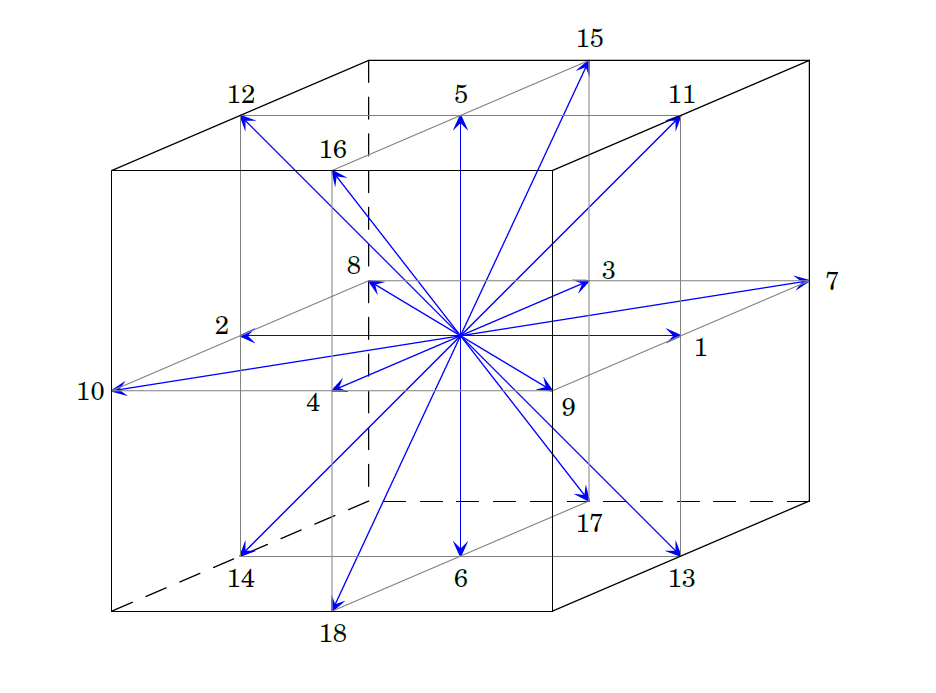
\includegraphics[width=0.5\textwidth]{img/d3q19}
  \caption{D3Q19模型离散速度}
  \label{fig:d3q19}
\end{figure}





%
%$\Omega_i$通常只由当前格点自己的各个速度方向的速度分布函数$f_i(\bm x, t)$决定,因此LBE是一种显式格式。
%在碰撞步,各个个格点的速度分布函数更新操作可以独立进行,并且只涉及到读取本身的信息,
%因此非常适合于细粒度的并行。

%传统的CFD方法如有限差分法、有限体积法、有限元法都是采用数值格式离散Navier-Stokes偏微分方程,
%得到一组线性方程组,然后采用数值线性代数的方法求解这组方程组从而得到流场在离散单元上的离散解。
%这些方法可以看做是“自顶向下”的方法,即已知描述流体运动规律的宏观控制方程,然后标准的偏微分
%方程求解方法来求解它们。而LBM与这些方法不同,它更类似于分子动力学方法(MD),即从微观上描述
%一群粒子的运动过程。在给定初始状态和演化规则的情况下,可以知道粒子在任一时刻的分布状态。
%但与MD描述每个真实分子的运动状态不同,LBM采用的是统计力学的方法,描述

\section{多松弛时间模型}
在LBGK模型中,各个方向的速度分布函数的松弛时间都是$\tau$,所以也被称作单松弛时间模型。
另一种常用的碰撞算子模型是多松弛时间模型(MRT), Lallemannd 和 Luo曾对这一模型做过
细致的理论分析,证明该模型比LBGK模型在参数选择自由度和数值稳定性方面具有更大优势,
并且物理原理更清晰。值得指出在LBGK在模拟多孔介质流动时,会得到绝对渗透率与流体
粘性相关联的非物理结果,而MRT模型则可以大大改善这一问题,Pan等人对这一问题做了详细算例验证
和分析\ucite{pan2006evaluation}。
MRT模型与LBGK模型不同之处在于它的碰撞过程是在矩空间中完成的。
碰撞前速度分布函数被一个正交变换矩阵$\bm M$映射到矩空间:
\begin{equation}
  m = \bm M \cdot \bm f
  \label{M_to_f}
\end{equation}
其中$m$为矩向量,对于D3Q19模型,$\bm M$为
  \renewcommand{\baselinestretch}{1.25}
\begin{displaymath}
\footnotesize
\bm M = \left(
\begin{array}{*{19}{@{\hspace{5pt}}r}}
 1 & 1 & 1 & 1 & 1 & 1 & 1 & 1 & 1 & 1 & 1 & 1 & 1 & 1 & 1 & 1 & 1 & 1 & 1 \\
 -30 & -11 & -11 & -11 & -11 & -11 & -11 & 8 & 8 & 8 & 8 & 8 & 8 & 8 & 8 & 8 & 8 & 8 & 8 \\
 12 & -4 & -4 & -4 & -4 & -4 & -4 & 1 & 1 & 1 & 1 & 1 & 1 & 1 & 1 & 1 & 1 & 1 & 1 \\
 0 & 1 & -1 & 0 & 0 & 0 & 0 & 0 & 0 & 0 & 0 & -1 & 1 & -1 & 1 & -1 & 1 & -1 & 1 \\
 0 & -4 & 4 & 0 & 0 & 0 & 0 & 0 & 0 & 0 & 0 & -1 & 1 & -1 & 1 & -1 & 1 & -1 & 1 \\
 0 & 0 & 0 & 1 & -1 & 0 & 0 & 1 & -1 & -1 & 1 & 0 & 0 & 0 & 0 & 1 & -1 & -1 & 1 \\
 0 & 0 & 0 & -4 & 4 & 0 & 0 & 1 & -1 & -1 & 1 & 0 & 0 & 0 & 0 & 1 & -1 & -1 & 1 \\
 0 & 0 & 0 & 0 & 0 & 1 & -1 & 1 & -1 & 1 & -1 & -1 & 1 & 1 & -1 & 0 & 0 & 0 & 0 \\
 0 & 0 & 0 & 0 & 0 & -4 & 4 & 1 & -1 & 1 & -1 & -1 & 1 & 1 & -1 & 0 & 0 & 0 & 0 \\
 0 & 2 & 2 & -1 & -1 & -1 & -1 & -2 & -2 & -2 & -2 & 1 & 1 & 1 & 1 & 1 & 1 & 1 & 1 \\
 0 & -4 & -4 & 2 & 2 & 2 & 2 & -2 & -2 & -2 & -2 & 1 & 1 & 1 & 1 & 1 & 1 & 1 & 1 \\
 0 & 0 & 0 & 1 & 1 & -1 & -1 & 0 & 0 & 0 & 0 & -1 & -1 & -1 & -1 & 1 & 1 & 1 & 1 \\
 0 & 0 & 0 & -2 & -2 & 2 & 2 & 0 & 0 & 0 & 0 & -1 & -1 & -1 & -1 & 1 & 1 & 1 & 1 \\
 0 & 0 & 0 & 0 & 0 & 0 & 0 & 0 & 0 & 0 & 0 & 0 & 0 & 0 & 0 & -1 & -1 & 1 & 1 \\
 0 & 0 & 0 & 0 & 0 & 0 & 0 & 1 & 1 & -1 & -1 & 0 & 0 & 0 & 0 & 0 & 0 & 0 & 0 \\
 0 & 0 & 0 & 0 & 0 & 0 & 0 & 0 & 0 & 0 & 0 & 1 & 1 & -1 & -1 & 0 & 0 & 0 & 0 \\
 0 & 0 & 0 & 0 & 0 & 0 & 0 & 0 & 0 & 0 & 0 & 1 & -1 & 1 & -1 & -1 & 1 & -1 & 1 \\
 0 & 0 & 0 & 0 & 0 & 0 & 0 & 1 & -1 & -1 & 1 & 0 & 0 & 0 & 0 & -1 & 1 & 1 & -1 \\
 0 & 0 & 0 & 0 & 0 & 0 & 0 & -1 & 1 & -1 & 1 & -1 & 1 & 1 & -1 & 0 & 0 & 0 & 0
\end{array}
\right)
\end{displaymath}
 \renewcommand{\baselinestretch}{1.5}
相应的矩向量为
\begin{displaymath}
 m=(\rho, e, \epsilon, j_x, q_x, j_y, q_y, j_z, q_z, 
3p_{xx}, 3\pi_{xx},p_{ww},\pi_{ww},p_{xy}, p_{yz}, p_{zx},m_x, m_y, m_z)
\end{displaymath}
其中各分量的意义及其对应的平衡态形式见参考文献\cite{pan2006evaluation},此处不再详细给出。
%其中$e$是能量,$\epsilon$是能量的平方,$\bm j=(j_x, j_y, j_z)$是动量,$\bm q=(q_x, q_y, q_z)$
%是热通量,$p_{xx},p_{ww}, p_{xy}, p_{yz}, p_{zx}$是与应力张量直接相关的矩,$\pi_{xx}, \pi_{ww}$
%是四阶矩,$m=(m_x, m_y, m_z)$是与速度有关的三阶矩。其中的$\rho$和$\bm j$是守恒矩。矩向量的平衡态
%$\bm m^{eq}$为
% m=(\rho, e, \epsilon, j_x, q_x, j_y, q_y, j_z, q_z, 
%3p_{xx}, 3\pi_{xx},p_{ww},\pi_{ww},p_{xy}, p_{yz}, p_{zx},m_x, m_y, m_z)
%\end{displaymath}


MRT模型中碰撞时先将$\bm f$转换到矩空间得到矩向量$\bm m$,
然后在矩空间完成碰撞,最后把碰撞更新后的$m$转换回速度分布函数$\bm f$,整个过程可以表示为
\begin{equation}
\Omega_i = \bm M^{-1} \bm S(\bm m - \bm m^{eq})
\end{equation}
其中$\bm S$为对角矩阵,其对角线上的各个元素为矩向量各分量的无量纲松弛时间, 其形式为
\begin{displaymath}
\bm S = diag(0,s_1,s_2,0,s_4, 0, s_4, 0, s_4, s_9, s_10, s_9, s_{10}, s_{13}, s_{13}, s_{13}, s_{16}, s_{16}, s_{16})
\end{displaymath}
通常取$s_9=s_{13}=s_\nu$, $s_\nu$与流体动力学粘性相关
\begin{equation}
\nu = c_s^2(\frac{1}{s_\nu}-\frac{1}{2})\delta t
\end{equation}
其它松弛时间可自由调节以获得更高的稳定性\ucite{d2002multiple}。


%%%%%%%%%%%%%%%%%%%%%%%%%%%%%%%%%%%%%%%%%%%%%%%%%%%%%%%%%%%%%%%%%%%%%%%%%%%%%%%%%%%%
\section{边界处理}
在迁移过程中,处于流场边界上的格点需要特殊处理,因为边界以外没有粒子迁移到这些格点,
LBM的边界处理的目标就是根据给定的宏观边界条件构造出这些未知的粒子分布函数。在这一节中
笔者主要讨论本文用到的三种边界处理格式,分别为周期性边界条件、反弹格式及郭照立提出的
非平衡外推格式\ucite{guo2002extrapolation}。

\begin{myDescription}
\item[周期性边界条件]
某些问题流场本身就有空间周期性, 这时可以只求解一个周期单元。这种边界处理在LB里面处理
非常容易,当前时间步从一侧流入流场的粒子就是上一时刻从另一侧流入流场的粒子。

\item[反弹格式]
反弹格式是来处理无滑移速度壁面最简单的,并且物理背景清晰。其基本想法是认为
靠经壁面的格点上的粒子在当前时间步流动到壁面并与壁面反弹后由其反方向弹回,在下一时间步
正好又回到这个格点。这种格式自动满足质量守恒和动量守恒。需要注意的是,标准
如果反弹格式中靠近壁面执行反弹的格点本身不执行碰撞更新操作,则称该格式为标准反弹格式,否则
为修正反弹格式,前者仅具有一阶精度,而后者具有二阶精度。另一种具有二阶精度的反弹格式为
Half-Way反弹格式,这种格式假设壁面正好位于格点连线之间。

\item[非平衡外推格式]
非平衡外推的基本思想是将边界格点上未知的分布函数分为平衡态和非平衡态部分,其中非平衡
部分,由临近的流场内部格点的非平衡部分一阶外推得到,而平衡态部分则根据给定的边界宏观量
来构造,构造过程缺少的宏观量也由临近的流场内部格点上的相应宏观量外推得到。这种格式整体
精度是二阶的\ucite{guoredbook}。
\end{myDescription}

%%%%%%%%%%%%%%%%%%%%%%%%%%%%%%%%%%%%%%%%%%%%%%%%%%%%%%%%%%%%%%%%%%%%%%%%%%%%%%%%%%%%
\section{多相/多组分LBE模型}\label{sec:lbm_multiphase}
宏观的相间相互作用本质上是组分中微观分子间的相互作用,因此如果能准确描述这种
分子间相互作用,则宏观多相/多组分复杂的流动现象会自然体现出来。LBM的微观本质和介观特点
决定了LBM也可以通过构造粒子间相互作用模型来模拟多相/多组分流动。目前在LBM中,描述粒子
间相互作用的方式有颜色模型、伪势模型、自由能模型和动力学模型。其中伪势模型又称Shan-Chen
模型,是由Shan和Chen于1993年提出的\ucite{sc93}。该模型假设流体粒子之间存在一种非局部的
相互作用,并通过引入一种势函数来描述这种相互作用,作用力的大小就是势函数的梯度。该模型
提出后,针对其存在的问题,又有多种改进模型被提出。本文所采用的多相多组分模型
\ucite{porter2012multicomponent}就是针对对Shan-Chen模型的一种改进。该模型主要解决了
Shan-Chen模型中平衡态密度和粘度相关的问题,并且能过模拟大粘度比的组分。下面将以该模型
为背景简要介绍运用LBM模拟多组分/多相问题的要点。

\subsection{组分间相互作用}
在原始的Shan-Chen模型中,组分间的相互作用力通过一个势函数来描述,
并且这个相互作用力对碰撞过程的影响通过校正有效平衡态速度来体现\ucite{sc93}。相互作用力的表达式为
\begin{equation}
\bm F_k(\bm x) = -\psi_k(\bm x)\sum_{\bar k}g_{k\bar k}\sum_i\psi_{\bar k}(\bm x+\bm c_i\delta t)\bm c_i
\label{sc_force}
\end{equation}
其中$\psi_k$是势函数,对于多组分模型通常就取为组分的密度即,$\psi_k = \rho_k$。$g_{k{\bar k}}$是反映
组分粒子间相互作用的系数。
在本文使用的这个模型中,每个组分所受到的合外力显式(explict force )的加到了其格子Boltzmann方程中\ucite{porter2012multicomponent},后文中称这种模型为EF模型。每个组分的LBE为
\begin{equation}
f_i^k(\bm x + \bm c_i\delta t) - f_i^k(\bm x, t)=\Omega_i^k(f(\bm x, t))+\frac{\Delta t}{2}
\left[ f_i^{F,k}(\bm x+\delta t, t+\delta t)+ f_i^{F,k}(\bm x, t)\right]
\label{ef_lbe}
\end{equation}
其中的$f_i^{F,k}$是粒子所受合外力引起的速度分布函数的改变,碰撞算子$\Omega_i$与单组分LBE形式相同。
$f_i^{F,k}$定义为
\begin{equation}
f_i^{F,k}=\frac{\bm F_k \cdot(\bm c_i - \bm u_{eq})}{\rho_k c_s^2}f_i^{eq,k}
\end{equation}
其中$\bm F_k$为组分$k$的粒子所受外力,包括组分间作用力。$\bm u^{eq}$是有效速度,定义为
\begin{equation}
\bm u^{eq} =  \sum_k\frac{\rho_k \bm u_k}{\tau_k}/\sum_k\frac{\rho_k}{\tau_k}
\end{equation}

方程\eqref{ef_lbe}右端包含新时间步的变量,所以是显式形式,通过做代换
$\bar f_i^k=f_i^k -\frac{\delta t}{2}f_i^{F,k}$,该方程可变为显式形式
\begin{equation}
\bar f_i^k(\bm x + \bm c_i\delta t) - \bar f_i^k(\bm x, t) 
=\frac{1}{\tau_k}\left[f_i^{eq,k}(\bm x, t) - \bar f_i^k(\bm x, t) - \frac{\delta t}{2}f_i^{F,k}\right]
+\delta t f_i^{F,k}
\end{equation}
每个组分的宏观量定义为
\begin{equation}
\rho_k = \sum_i\bar f_i^k, \quad \rho_k \bm u_k = \sum_i \bar f_i^k \bm c_i + \frac{\delta t}{2}\bm F_k
\end{equation}
混合流体的真实速度为
\begin{equation}
\bm u =\frac{\sum\nolimits_k\rho_k\bm u_k}{\sum\nolimits_k\rho_k}
\end{equation}
流体状态方程为
\begin{equation}
  p=c_s^2 \sum_k\rho_k + \frac{c_0}{2}\sum_{k\bar k}g_{k\bar k}\psi_k\psi_{\bar k}
  \label{EOS}
\end{equation}

值得指出的是在原文献\ucite{porter2012multicomponent}中,为能模拟大粘度比组分,
式\eqref{sc_force}表达为
\begin{equation}
\bm F_k(\bm x) = -c_0\psi_k(\bm x)\sum_{\bar k}g_{k\bar k}\nabla \psi_{\bar k}(\bm x)
\label{sc_force_m}
\end{equation}
式中$c_0$是个常速,对于D3Q19格子模型,$c_0 =6$,式中的梯度算子
用具有较好各向同性的的高阶差分算法替代。但考虑到GPU上对显存访问的特殊要求(见\ref{sec:cuda_principle}节中的
解释),我们在后文中实现的多组分GPU程序使用的都是一阶中心差分格式。

\subsection{流固界面相互作用}
流固边界处的流体格点的某些方向上的相邻格点可能是固体格点,为反映固体边界对各组分的作用,
可以将固体格点等效为另一种假想的组分,其密度为常数$\rho_s$,它与流体组分间的相互作用系数
用$g_{ks}$替代,$g_{ks}$大小反应组分$k$对该固体表面的润湿性,通过调整不同组分的$g_{ks}$
控制相界面接触角的大小\ucite{pan2004lattice}。

%在多组分流中,每个组分有自己的分布函数,并且它们的演化过程都满足格子Boltzmann方程
%\begin{equation}
%f_i^k(\bm x + \bm c_i\delta t) - f_i^k(\bm x, t)=\Omega_i^k(f(\bm x, t))
%\end{equation}
%其中$k$表示组分,由于本文只涉及到两组分,所以$k$取值为$1$或$2$。当然也很容易扩展成更多
%组分。如果采用单松弛碰撞算子模型则有
%\begin{equation}
%\Omega_i^k = \frac{f_i^{eq,k}(\bm x, t) - f_i^k(\bm x, t)}{\tau_k}
%\label{srt_multi}
%\end{equation}
%其中$\tau_k$表示组分$k$的无量纲松弛时间,同单组份的LBM一样分别于两种组分的动力学粘性相关,
%式中中各组分$f_i^{eq,k}$平衡态定义如下
%\begin{equation}
%  f_i^{eq,k} = \omega_i \rho_k 
%  \left[ 1 
%    + \frac{\bm c_i \cdot \bm u_k^{eq}}{c_s^2}
%    + \frac{(\bm c_i \cdot \bm u_k^{eq})^2}{2c_s^4}
%    - \frac{u^{eq}\cdot u^{eq}}{2c_s^2}
%    \right]
%  \label{feq_multi}
%\end{equation}
%每个组分的宏观量$\rho_k$、$\bm u_k$依然按各自的分布函数统计出来,即
%\begin{equation}
% \rho_k = \sum_i f_i, \quad \rho_k \bm u_k =  \bm c_i f_i
%\end{equation}
%式\eqref{feq_multi}中的$\bm u^{eq}$是根据组分间相互作用力校正过了的有效速度
%\begin{equation}
% \rho_k \bm u
%\end{equation}

%%%%%%%%%%%%%%%%%%%%%%%%%%%%%%%%%%%%%%%%%%%%%%%%%%%%%%%%%%%%%%%%%%%%%%%%%%%%%%%%%%%%
\section{小节}
本章介绍了LBM基本原理。在第一节中介绍了常用的D2Q9和D3Q19格子模型,以及单松弛时间(LBGK)模型,
第二节介绍了后文将要使用的多松弛时间(MRT)模型,第三节介绍了常用的LB边界处理方法。
第四节详细介绍了本文所使用多相LB模型。









%%%%%%%%%%%%%%%%%%%%%%%%%%%%%%%%%%%%%%%%%%%%%%%%%%%%%%%%%%%%%%%%%%%%%%%%%%%%%%%%%%%%
% GPU & CUDA
\chapter{GPU构架及CUDA编程技术}
\section{GPU:大规模并行处理器}GPU最开始是为图形渲染而设计的,它负责处理计算机系统的图形渲染任务。
图形渲染操作具有高度数据并行性,一般要对大量图形元素执行相同的操作,因此非常适合在SIMD(单指令多数据)
型并行构架上并行实现。其另一个特点是对每个元素执行的操作较为简单因此适合于细粒度并行。
GPU的设计正体现了图形处理的这些特点,现代GPU包含大量功能较为简单的处理单元和存储控制单元,
通过在这些处理单元同时执行大量线程可以达到掩藏访存延迟的目的,
这与CPU设计思想不同,CPU核心只有一个具有复杂控制功能的处理单元,
并用大缓存来掩藏访存延迟。
图\ref{fig:gpu_cpu_arch}所示为CPU和GPU的晶体管使用情况。
\begin{figure}[htpb]
  \centering
  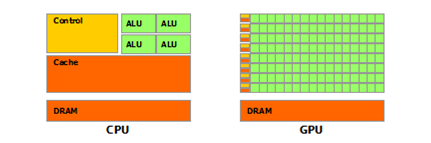
\includegraphics[]{img/gpu_cpu_arch}
  \caption{GPU和CPU的晶体管结构 \footnotesize 来源:NVIDIA}
  \label{fig:gpu_cpu_arch}
\end{figure}
由于图形渲染任务的并行性,设计GPU时可以简单的通过增加晶体管数量来扩充其计算性能和存储带宽。
图\ref{fig:performance}和\ref{fig:bandwidth}所示为CPU和GPU计算速度和存储发展情况比较。
可以看出,目前主流的GPU比同期CPU计算速度和存储带宽都高出很多倍。

\begin{figure}[htb]
  \centering
  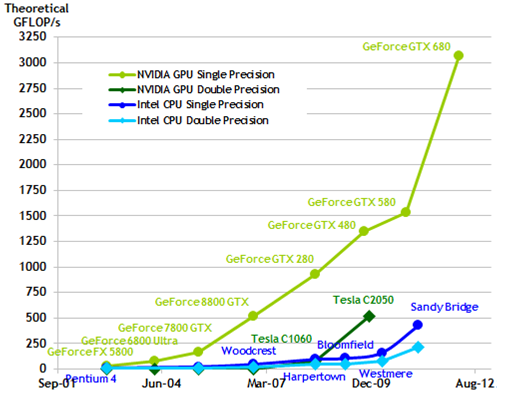
\includegraphics[]{img/performance}
  \caption{GPU和CPU的每秒浮点运算次数 \footnotesize 来源:NVIDIA}
  \label{fig:performance}
\end{figure}

\begin{figure}[htb]
  \centering
  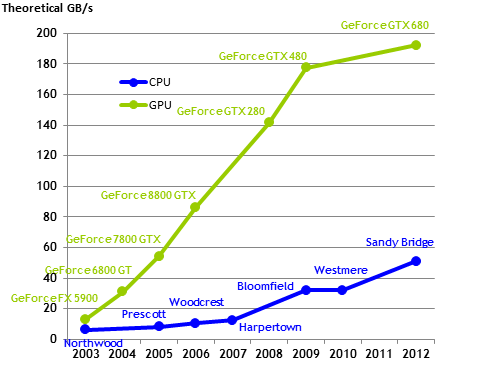
\includegraphics[]{img/bandwidth}
  \caption{GPU和CPU的的存储带宽 \footnotesize 来源:NVIDIA}
  \label{fig:bandwidth}
\end{figure}

\section{GPU构架}\label{sec:gpu_arch}
图形显卡在硬件上主要由GPU芯片、显存以及PCI总线组成。目前市场上主流的显卡主要由
两家公司设计\---NVIDIA和AMD,二者在结构和功能部件名称上存在一些差别。
由于本文研究的是NVIDIA公司的CUDA技术构架下的GPGPU
编程,所以后文对GPU结构和功能的介绍均以NVIDIA公司的显卡为例,
具体的,我们将使用NVIDIA公司的高端显卡\---Tesla C1060。

GPU芯片上集成了大量处理单元,是显卡的计算功能部件。Tesla C1060 显卡使用的是一个GT200 GPU核心。
核心中的处理单元按两层结构组织\---多处理器(SM)和流处理器(SP),其中一个SM包含多个SP。
GT200核心上有30个SM,每个SM包含有8个SP,因此一共是240个SP。每个SP有一个单精度计算单元,每个
SM拥有一个双精度计算单元。SP工作频率为1296MHz,SP每个时钟周期能执行3次单精度浮点数操作,
每个双精度计算单元每个时钟周期能执行2次双精度浮点数操作。因此GT200核心理论单精度计算能力为
$240\times 1296\text{(MHz)}\times 3\text{(flops)} \approx 933\text{Gflops}$, 双精度计算能力为
$30\times 1296\text{(MHz)}\times 2\text{(flops)} \approx 78\text{Gflops}$。 
GT200核心的双精度计算能力是单精度的$1/12$,因此其计算性能的优势主要体现在单精度浮点数计算上。
在NVIDIA公司后来推出的Fermi构架和最新推出的Kepler构架的GPU上,双精度浮点数计算速度大为改善,
可以达单精度的$1/2$。
%每个SM上有16KB的共享存储器(shared memory),
%它是一种高速存储器,SP访问它只有2-4个是·
值得指出的是,虽然SP是GPU核心实际的计算单元,但由于SP没有独立的寄存器和取指、调度单元,
所以SP并不是一个独立的类似CPU的执行单元。

显存作用类似于CPU构架中的内存,是GPU主要存储器。Tesla C1060 显存大小为4GB。多处理器通过
8个存储控制器与显存相连,每个存储控制器位宽为64bit,所以显存总位宽是$8\times 64\text{bit}=512\text{bit}$。
存储单元工作频率为2214MHz,理论外部存储带宽为$512\times 2214\text{Mhz}\approx142\text{GB/s}$。和CPU相同,
由于存在较大的访存延迟,GPU的外部存储带宽往往是程序性能的一个限制因素。

PCI-E总线是显存与主板芯片组的数据通道,总线带宽根据所采用PCI-E规范版本及通道数量不同而有所差异。
通常能提供上下各数GB/s的带宽。总线带宽比显存外部带宽带宽低得多,容易成为程序性能的瓶颈,
所通常要尽量减少CPU主存与GPU显存之间的频繁地数据传输。

\section{CUDA编程模型}
CUDA技术的提出,大大简化了通用GPU计算程序的开发。在CUDA技术提出之前,要想利用GPU做通用计算,
编程人员必须掌握计算机图形API和图形硬件细节,并将自己的应用程序按照计算机图形学里面的概念
来描述和编码,这种方式繁琐而不自然。 2007年,NVIDIA推出了CUDA技术,与传统GPGPU不同,CUDA将
图形学API隐藏起来,直接C语言基础上扩展,它允许编程者自己编写一种类似普通C函数的\textit{Kernel}函数
在SP上执行,从而利用GPU的大规模并行计算能力。另外它还提供线程执行控制、存储器管理等功能并以运行时库函数
的方式供CPU上执行的普通函数调用。下面介绍CUDA技术中的几个关键概念。
\begin{myDescription}
\item[Host与Device] 一个完整的CUDA程序包含在CPU执行的部分和在GPU上执行的部分。CPU端被称作\textit{Host}端,
  GPU端被称为\textit{Device}端。Host端运行的代码是标准的C语言(或Fortran、Python等其它语言),而Device端
  运行的代码是由扩展的C语言编写的,并被封装在一个在声明时由\verb+__global__+修饰的函数中,这种
  函数被称作\textit{Kernel}。当Host端程序运行到要调用Kernel时,编译好的Kernel代码被装载到Device端,开始
  由GPU核心执行。图\ref{fig:cuda_program}示例为CUDA程序的执行过程。
  \begin{figure}[htpb]
    \centering
    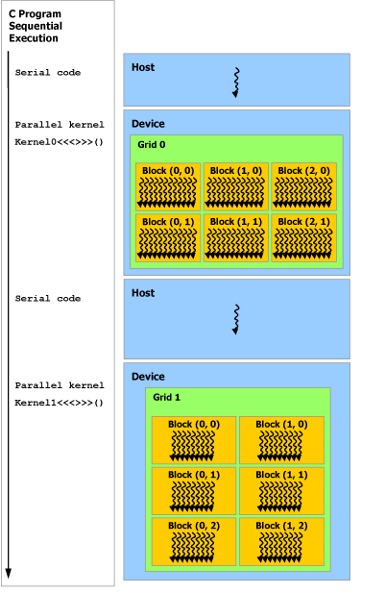
\includegraphics[]{img/cuda_program}
    \caption{CUDA程序执行流程 \footnotesize 来源:NVIDIA}
    \label{fig:cuda_program}
  \end{figure}

\item[线程] 
线程(thred)是CUDA的核心概念,它是与流处理器SP相对应的逻辑
上的概念,可以理解为GPU代码的一条逻辑执行主线。
在已经充分掩藏了访存延迟的情况下,GPU核心里面的每个SP都同时运行着一个线程。
这种线程的粒度相对于CPU上的线程而言非常小,并且通常没有复杂的逻辑判断分支执行路径。


\item[Block与Grid] 运行Kernel的线程按层次被组织为线程块\textbf{Block}与线程块网格\textbf{Grid}。
  通常整个求解域被映射到一个Grid上,并被划分为细小的单元,Grid中的每个线程负责处理一个单元。
  Grid中的线程又按划分为Block,划分方式可以是一维、二维或者三维,相应的Block也可以是一维、二维或三维的。
  Grid和Block的大小(即Grid各维度上Block的数量和Block各维度上线程数量)分别由\verb+dim3+类型的参数指定。这种变量
  有三个整数分量,分别指定Grid或Block在各维度上元素的个数(二维可以看做特殊的三维情况,及第三个分量为1)。
  在调用Kernel时指定这些参数,这些参数并以内建全局变量的形式出现在Kernel函数中,分别为\verb+gridDim+
  和\verb+blockDim+。在Kernel中还有两个\verb+uint3+类型的局部变量\--- \verb+blockIdx+和\verb+threadIdx+,
  它们也有三个整数分量。\verb+blockIdx+记录当前线程所属Block在Grid中的位置,\verb+threadIdx+记录当前线程
  在其Block中的位置。每个线程可以根据这些变量确定其在grid中的位置,进而确定其所处理的数据在显存中的位置。
  位于同一个Block中的线程共享部分高速存储器\---共享内存。CUDA还提供\verb+__syncthreads()+函数来实现块内线程同步。
  通过共享内存和线程同步,CUDA提供了一种简单的线程间通信能力。Block中的线程又隐式的被划分为若干个\textit{wrap},
  wrap的概念在CUDA源程序中没有体现,但线程执行和访存时是按wrap为单位进行的。
\end{myDescription} 

代码1提供一个完整的CUDA程序实例\---矩阵$\bm A$和$\bm B$的求和运算,上述各种概念在其中已有体现。
\begin{Code}
\begin{lstlisting}
#define N 1024
#define BX 16
#define BY 16
float A_h[N][N], B_h[N][N],  C_h[N][N];//Host`端存数组` 
float *A_d, *B_d, *C_d;//`Device端数据指针`
//Kernel`函数定义`
__global__ void
 matrixAdd(float A[N][N], float B[N][N], float C[N][N]) 
{
	int x = blockId.x*blockDim.x + threadIdx.x;
	int y = blockId.y*blockDim.y + threadIdx.y;
	C[y][x] = A[y][x] + B[y][x];
}  
int main()
{
	...
	//Host`端初始化`A_h, B_h
	...
	//Device`分配显存存储Device端数据`
	cudaMalloc((void**)A_d, sizeof(float)*N*N);
	cudaMalloc((void**)B_d, sizeof(float)*N*N);
	cudaMalloc((void**)C_d, sizeof(float)*N*N);
	//`拷贝Host端数据到Device端`
	cudaMemcpy(A_d, A_h, cudaMemcpyHostToDevice);
	cudaMemcpy(B_d, B_h, cudaMemcpyHostToDevice);
	dim3 GRID(BX, BY);//`定义Grid尺寸`
	dim3 BLOCK(N/BX, N/NY);`定义Block尺寸`
	//`调用`Kernel
	matrixAdd<<<GRID, BLOCK>>>(A_d, B_d, C_d);
	//`将结算结果`C`拷回Host端`
	cudaMemcpy(C_h, C_d, cudaMemcpyDeviceToHost);
	...
	//Host`端的后续操作`
	...
	return 0;
} 
\end{lstlisting}  
\caption{一个实现矩阵相加(C=A+B)的CUDA程序}
\end{Code}


%\section{存储器类型}
和Host端类似,在Device端也存在各种不同的存储器类型。它们的大小、访问开销各不相同。合理的使用用它们
是提高CUDA程序性能的关键,这里我们介绍常用的几种存储器类型。
\begin{myDescription}
\item[全局存储器] 
全局存储器(global Memroy)位于显存并占据了显存的绝大多数空间,
功能类似于Host段的主存,用来存贮主要的计算数据,如LBM中的分布函数、宏观量等。全局存储器通
过调用\texttt{cudaMalloc}来分配,通过调用\texttt{cudaMemcpy}实现全局内存与Host内存之间的数据传输。
全局内存的访问开销相对其他类型的存储器非常大,通常有几百个时钟周期延迟。同一个wrap中的线程
访问全局存储器时,若访存地址满足对齐要求并且相邻线程访问的地址连续,会被合并为一次访问请求,
只需要进行一次数据传输,否则会及进行多次数据传输,显存带宽会大幅下降,在早期的GPU上,这一效应
尤为明显。

\item[寄存器] 寄存器(register)是GPU片上的一种高速存储器,Kernel函数声明的临时变量通常就是这种类型。
在GT200核心中,每个SM寄存器大小为16KB,SM同时为多个线程维护一份寄存器,所以每个线程分配到的寄存器
数量非常有限。若Kernel中寄存器用量超过其上限,数据就会被存储到局部存储器,后者访存开销相当大。

\item[共享内存] 共享存储器(shaared memory)是位于GPU芯片上的一种高速存储器,几乎没有访存延迟,
它可以被同一个Block中的所有线程访问。共享内存数量较少,是一种稀缺资源,如GT200核心中每个SM的
的共享内存数量为16KB。在Kernel函数中通过\texttt{\_\_shared\_\_}修饰声明。

\item[常数存储器] 常数存储器(constant memory)是一种只读的存储器,
  通常用来存储少量计算参数。常数存储器也较少,GT200核心只有64KB大小。

\item[局部存储器] 局部存储器位于显存,当寄存器用完时会自动被使用,访问开销与全局存储器相同。
\end{myDescription}

\section{CUDA程序优化的基本原则}\label{sec:cuda_principle}
为充分利用GPU提供的大量处理器和存储带宽,设计和优化程序时要遵守一些基本原则,否则
GPU的实际性能会大为降低,下面列出一些常见的要求
\begin{itemize}
  \item Block大小为应该是32的整数倍;
  \item 控制Kernel汇总共享内存和寄存器用量,保证SM上至少
    能容纳2个活动的Block和6个活动的wrap,否则不能充分
    掩藏全局存储器访问延迟;
  \item 合理选择Block尺寸,此要求通常与上一条要求相互矛盾,
    实际设计时要根据计算实验来确定最优Block尺寸;
  \item 尽量保证访存满足地址对齐和连续的要求。
\end{itemize}

\section{小结}
本章前半部分介绍了GPU的基本构架和相应结构的功能,比较了其与CPU构架的差异,
并揭示了GPU之所以具有大规模并行能力的底层原因。本章后半部分主要主要介绍了
CUDA技术的基本概念,涉及到了CUDA技术的线程层次结构和存储器类型,理解这些
基本概念以及各种存储器的差异和使用要求是设计出高效率CUDA程序的前提。最后
我们列出了CUDA程序优化的基本原则,我们将在后面章节根据这些原则的指导设计
和优化LBM模拟的CUDA程序。



%%%%%%%%%%%%%%%%%%%%%%%%%%%%%%%%%%%%%%%%%%%%%%%%%%%%%%%%%%%%%%%%%%%%%%%%%%%%%%%%%%%%
% LBM & CUDA
\chapter{LBM在GPU上实现的基本方法}
本章介绍了目前文献中常见的LBM在GPU上的实现方法,着重讨论了影响程序性能的因素,并指出了其基本优化策略。
随后我们分别编制了模拟顶盖驱动二维方腔流和外力驱动三维方截面直管道流的GPU程序,在验证了程序正确性后
我们对其运行速度做了测试和分析。

\section{LBM在GPU上实现的基本方法}\label{optimize}
%LBM计算时间主要消耗在碰撞、迁移和统计宏观量等过程,所以只需将这些过程在GPU上实现。
由于GPU和CPU的构架存在巨大差异,很多适用于CPU的优化技术在GPU上可能根本就行不通,甚至
适得其反。例如CPU的LB程序中通常要避免数组的第一个维度大小为2的幂次,这是考虑到CPU缓存效率
的缘故\ucite{wellein2006single},而在GPU上情况却恰恰相反。下面将从LBM算法的特点结合GPU构架
特点来分析在GPU上实现高效LBM计算应该采取的策略。

在LBM计算过程中,每个格点
速度分布函数方向很多,但其碰撞步执行的计算却很简单,在迁移步甚至没有计算而只是简单的数据
加载与存储,因此LBM的计算访存比较大,在已经充分优化的情况下,程序的性能瓶颈还是在访存带宽,
并且在CPU上和GPU上都是如此\ucite{tolke2010implementation}。考虑到这一特点,LBM在GPU上的实现
及优化目标为最大限度发挥GPU的带宽优势,即尽量提高访存效率。下面将从数据布局和存储器使用方面
介绍LBM在GPU上实现的关键之处。

\subsection{优化数据布局}
%为了实现全局存储器的连续访问
在CPU上实现LBM时,速度分布函数(PDF)在内存中有两种最为常见的布局方式\---结构数组
(Arrays of Structure, AoS)和数组结构(Structure of Arrays,SoA)\ucite{wellein2006single}。
前者是指每个格点的$q$个PDF在内存中是连续排布的,而后者是指不同格点同一方向的PDF在
内存中是连续排布的。如果用C语言的数组记法表示,对于前者分布函数声明为\verb+f[NZ][NY][NX][Q]+,
而对于后者则为\verb+f[Q][NZ][NY][NX]+。在GPU实现时,为了保证相邻线程在同一时刻访问全局内存的
地址是连续的,只能采用后一种形式,即SoA。

\subsection{减少全局内存访问}
LBM计算在逻辑上可以分为三个步骤即碰撞、迁移、更新宏观量,如果分开执行这些操作,
则会多次从全局内存加载和存储数据。事实上利用LBM是一种显式方法这个特点,这三个逻辑
步骤可以合并在一个Kernel中执行。
通常在全局内存上开辟有两套PDF数组,如\verb+F0+和\verb+F1+,在一个时间步,每个格点
从\verb+F0+中加载自己的PDF,随后计算宏观量,然后执行碰撞,并将新的PDF写入到
\verb+F1+中相邻格点对应的位置,在下一时间步执行相同操作,不过读取和写入位置置换,
即从\verb+F1+中读取,碰撞后写入\verb+F0+。
注意在上述方法中迁移步已经掩藏在向周围点写入新PDF的过程中了。

\subsection{利用共享内存辅助迁移过程}\label{sec:cuda_share}
在迁移过程中每个格点不可避免地要从临近格点写入PDF,如果临近格点的$X$坐标(这里假定
按\verb+f[Q][NZ][NY][NX]+形式开辟数组)与自己不同,则写入过程肯定有一个\verb+sizeof(type)+
的偏移,因而不能不满足内存对齐要求,实际显存带宽会大为下降。目前常见的做法是用共享内存
辅助迁移。即格点首先将自己的PDF读到自己的共享内存中,完成碰撞操作后从共享内存将数据写
回全局内存,穿出Block边界的PDF正好可以临时存在Block另一侧空出的位置,
图\ref{fig:share_shift}所示为向右迁移的情况。
写会过程中从共享内存读的是相邻格点的数据,而写入全局内存时的是写到自己的位置。
总体上看,读写全局内存时都满足内存地址对齐要求,理论存储效率可以达到100\%。
\begin{figure}[htb]
  \centering
  \begin{tikzpicture}
    \matrix (block) [matrix of nodes, row sep=2.0em ,nodes={draw,  minimum width=2em, anchor=center} ]
    {
      0 & 1 & 2 & 3 \\
      0 & 1 & 2 & 3 \\
      0 & 1 & 2 & 3 \\
    };

    \draw (block-1-1.west) + (-1.0, 0) node {\hei \small 全局内存};
    \draw (block-2-1.west) + (-1.0, 0) node {\hei \small 共享内存};
    \draw (block-3-1.west) + (-1.0, 0) node {\hei \small 全局内存};

    \draw[->,thick] (block-1-1.south) -- (block-2-1.north);
    \draw[->,thick] (block-1-2.south) -- (block-2-2.north);
    \draw[->,thick] (block-1-3.south) -- (block-2-3.north);
    \draw[->,thick] (block-1-4.south) -- (block-2-4.north);

    \draw[->,thick] (block-2-1.south) -- (block-3-2.north);
    \draw[->,thick] (block-2-2.south) -- (block-3-3.north);
    \draw[->,thick] (block-2-3.south) -- (block-3-4.north);
    \draw[->,thick] (block-2-4.south) -- (block-3-1.north);
  \end{tikzpicture}
  \caption{利用共享内存辅助迁移}
  \label{fig:share_shift}
\end{figure}

\begin{figure}[htpb]
  \centering
  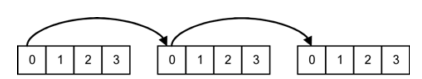
\includegraphics[]{img/exchange}
  \caption{\textbf{LBExchange}执行过程}
  \label{fig:lbexchange}
\end{figure}

由于在迁移过程中穿越Block边界的PDF没有被存到显存中正确的位置,所以在执行完碰撞步的Kernel
后还要紧跟着调用另外一个Kernel来完成迁移步,这里我们按原文献命名为\textbf{LBExchange}。
它的作用就是交换这些没有被迁移到正确位置的PDF。在三维情况,由于存储空间限制,不可能
所有方向网格数都很大,如不会都超过$128$或$256$,这时正好可以让一个相应大小的一维Block
处理网格数最小的方向上的“一条”格点,
这时可以不用执行\textbf{LBExchange} Kernel,而只需做一般的边界处理。
\ref{sq}节中的方截面直管道流动模拟
就利用了这个特点。

\section{验证算例及性能测试} \label{sec:speed_standard}
这一节简要列出利用上节所述方法实现的不同算例GPU程序的程序性能,并将计算结果与相关文献或解析解做了对比
以验证程序的正确性。
\subsection{计算环境及程序性能测量方法}
本工作使用的计算环境一台服务器搭载Tesla C1060型GPU的服务器,GPU标配显存4GB,
CPU为Intel Xeon X5550 8核处理器,操作系统为CentOS 5.9 64bit版,CUDA工具箱版本为3.2。
%使用Intel 的icc编译器,版本号为12.0.2。
%PC机搭载GeForce系列GTX480 GPU,CUDA工具箱版本为5.0,CPU为 AMD Athlon II X4 640。
本文中所有CPU程序均为串行程序,使用icc V10.1编译器编译,编译选项加上了\verb+-fast+。

衡量LBM程序速度的标准单位是MLUPS(Million Lattice Updates Per-second),
意为每秒百万节点更新数。按照这个单位,程序运行速度其定义为
\begin{equation}
  \text{Speed} = \frac{N_{\text{total}}\times T_{\text{LB}}}{10^6\times t_{\text{comput}}} \text{(MLUPS)}
  \label{mlups}
\end{equation}
其中$N_{\text{total}}$表示流场中格点总数,$T_{\text{LB}}$表示总的LB演化步数,
$t_{\text{comput}}$表示计算$T_{\text{LB}}$步所消耗的时间。
考虑多孔介质流动情况时,还有一个只考虑流体格点的衡量单位\---
MFLUPS,其定义与MLUPS相比只是分子的$N_{\text{total}}$换为流体格点总数。
因为多孔介质中存在大量不参与计算的固体格点,所以这个单位才能真实反映计算速度。

这里我们指出在计算GPU程序相对于CPU程序加速比时,CPU程序性能对加速比影响很大(作为分母),
而实际CPU程序执行的速度在相当程度上取决于CPU性能和所使用的编译器及编译选项,所以笼统的
指出GPU程序的加速比并能不准确放映GPU程序的加速效果。在后文的性能测试中我们主要
以MLUPS和MFLUPS为单位衡量GPU程序的绝对速度。

\subsection{二维方腔流}
二维方腔流边界条件简单,但是随雷诺数增大,却可以产生复杂的涡结构,因此被广泛地
用作验证程序正确性的标准算例\ucite{ghia1982high}。
这里我们采用的方腔流几何结构如图\ref{fig:ldc_a}所示,方腔四边长都为1.0m,空腔上边界以恒定速度$U=0.1\text{m/s}$水平向右移动。
我们对比了雷诺数为400时的GPU程序计算结果与Ghia\ucite{ghia1982high}等人的用多重网格方法计算得出的结果,
并将GPU程序和对应的CPU程序计算速度作了对比。

我们采用的是标准D2Q9 LBGK模型,固壁采用半反弹格式,上边界采用非平衡外推格式,网格数为$256\times 256$,
在GPU上采用单精度计算,收敛标准为
\begin{equation}
  \frac{\sqrt {\sum\nolimits_{ij}{| \bm u_{ij}^{n+1000}- \bm u_{ij}^{n} |^2}}}{\sqrt{\sum\nolimits_{ij}{|  \bm u_{ij}^{n} |^2}}}\le 1.0\times {{10}^{-6}}
  \label{convege}
\end{equation}
表示相邻1000步直间速度场的相对误差小于$1.0\times 10^{-6}$。 
图\ref{fig:ldc_b}所示为流场稳定后的流线图,可以发现有三个涡结构分别出现在方腔中心和左、右下角。表
\ref{tab:ldc}列出了本文计算出的涡中心位置以及Ghia\ucite{ghia1982high}的结果,可以看出本文结果和Ghia
的结果相差很小。
\begin{figure}[htb]
  \centering
  \subfigure[二维方腔流示意图]{
    \begin{minipage}[b]{0.4\textwidth}
      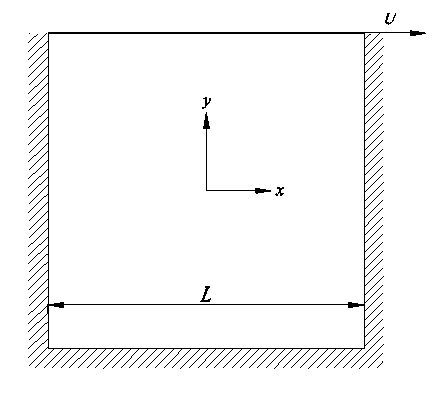
\includegraphics[width=1\textwidth]{img/ldc}
      \label{fig:ldc_a}
    \end{minipage}
  }
  \subfigure[$Re=400$时稳定后流线图]{
    \begin{minipage}[b]{0.38\textwidth}
      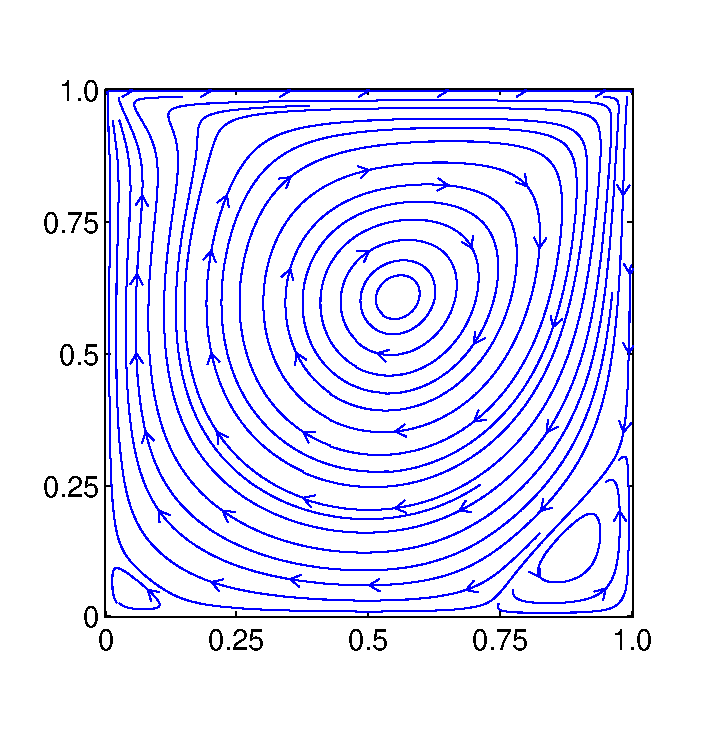
\includegraphics[width=1\textwidth]{img/ldc_stream}
      \label{fig:ldc_b}
    \end{minipage}
  }
  \caption{二维方腔流}
\end{figure}

\begin{table}
  \centering
  \begin{tabular}{*{7}{c}}
    \toprule
涡    & \multicolumn{2}{c}{一级涡} & \multicolumn{2}{c}{二级涡} & \multicolumn{2}{c}{三级涡}  \\ \cline{2-3} \cline{4-5} \cline{6-7}
位置    & $x_1$ & $y_1$              & $x_2$ & $y_2$              & $x_3$ & $y_3$          \\ \midrule
本文& $0.5543$ & $0.6070$        & $0.8889$ & $0.1235$        & $0.0522$ & $0.0475$        \\ \hline
Ghia& $0.5547$ & $0.6055$        & $0.8906$ & $0.1250$        & $0.0508$ & $0.0469$        \\ \bottomrule
  \end{tabular}
  \caption{$Re=400$时,各级涡中心的位置}
  \label{tab:ldc}
\end{table}

我们发现Block的大小(本文采用的Block是一维的)和总体网格规模对计算速度都有影响,图\ref{fig:ldc_speed}所示为
不同Block大小和不同网格规模时的计算速度,可以发现GPU最快速度快达到924MLUPS,而与之相比,我们的CPU
程序速度为7.5MLUPS,可见GPU程序加速比达到了123倍。

\begin{figure}[htb]
  \centering
  %\psfig{figure=img/ldc_speed}
  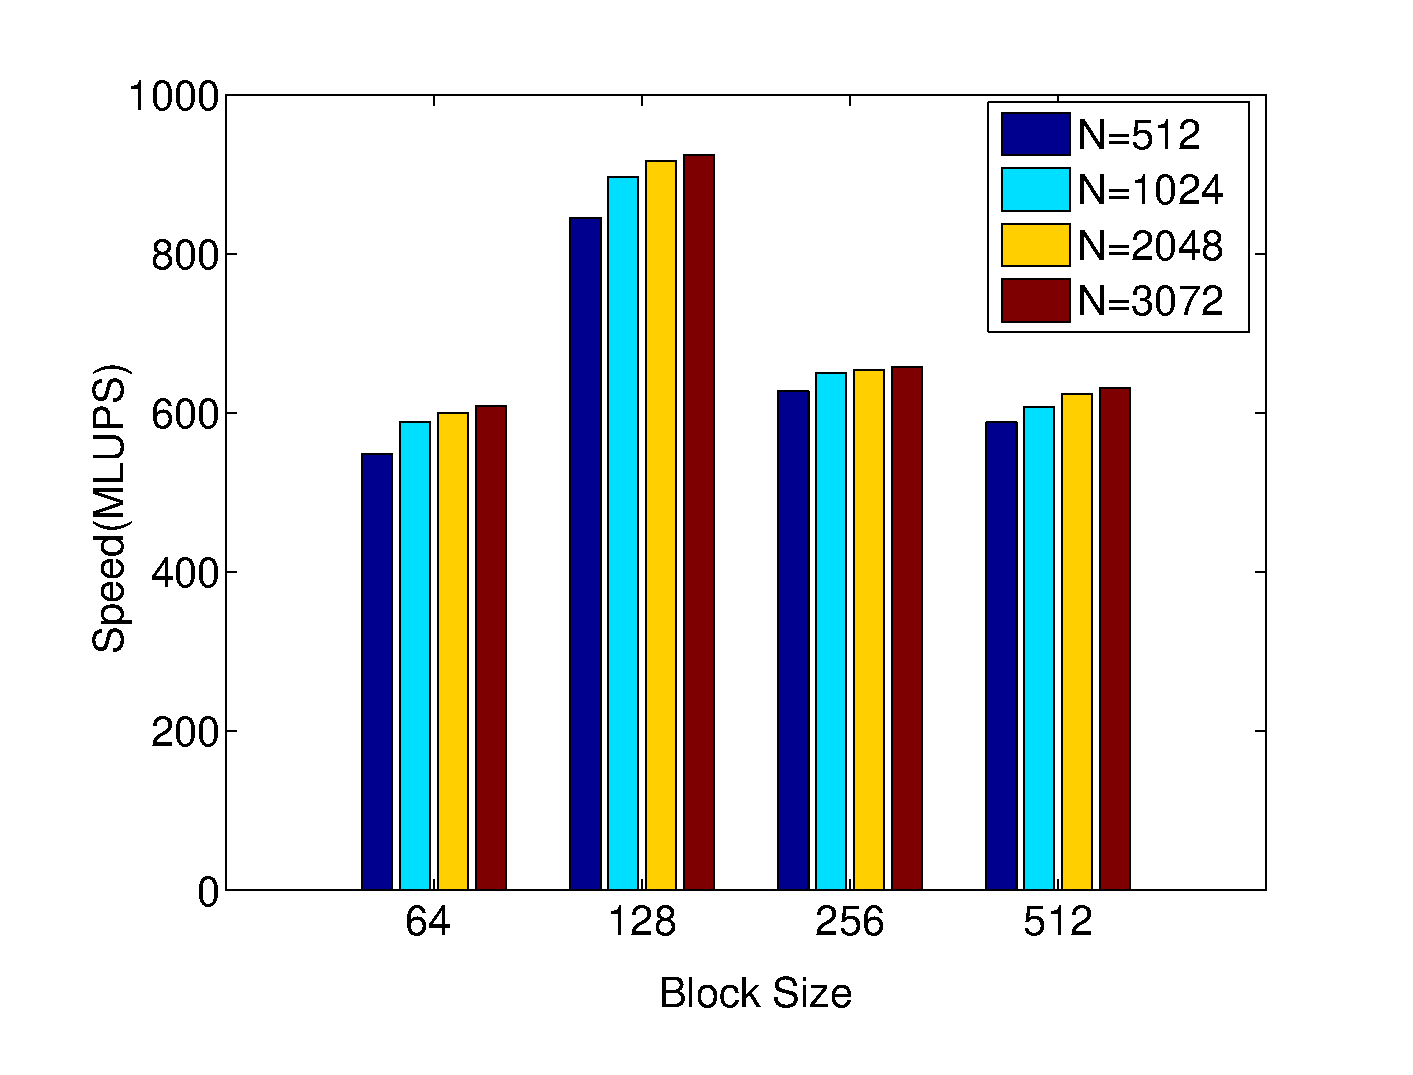
\includegraphics[width=0.8\textwidth]{img/ldc_speed}
  \caption{网格规模和不同Block尺寸对计算速度的影响}
  \label{fig:ldc_speed}
\end{figure}

\subsection{方形截面直管道流动}\label{sq}
本小节将依然使用\ref{optimize}节中描述的方法模拟三维方形截面直管道流动,
如图\ref{fig:sq}所示,这种流动类似于二维的
泊肃叶流动,流体由沿管道方向的外力$\bm F$驱动。
由于流动沿管道方向具有周期性,所以管道长度不影响截面速度分布。
截面流向速度分布只取决于外力大小$\bm F$和管道宽度$a$,其级数解析解为
\begin{equation}
  u(x, y) = U_0\sum_{i=1}^{\infty}(-1)^i\left(1-\frac{\cosh(\pi xi/a)}{\cosh(\pi i/2)}\right)\frac{\pi yi/a}{i^3}
  \label{sq_ana}
\end{equation}
其中$U_0=\frac{4aF}{\nu \pi^3}$。

\begin{figure}[htb]
  \centering
  \subfigure[几何结构]{
    \begin{minipage}[b]{0.6\textwidth}
      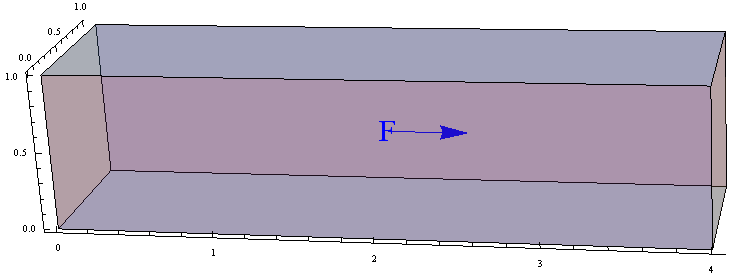
\includegraphics[width=0.9\textwidth]{img/sqpng}
      \label{fig:sq}
    \end{minipage}
  }
  \subfigure[管道截面示意图]{
    \begin{minipage}[b]{0.2\textwidth}
      \begin{tikzpicture}[scale=0.6]
        \draw[fill=gray!20]  (-2,-2) rectangle (2,2);
        \draw [<->,very thick] (0,1) node (yaxis) [above] {$y$} |- (1,0) node (xaxis) [right] {$x$};
        \node at (-2.2, 0) {\Large $a$};
        \node at (-0.3, -0.3) {\large $0$};
      \end{tikzpicture}
      \label{fig:sq_sec}
    \end{minipage}
  }
  \caption{外力驱动方截面直管道流}
\end{figure}
数值模拟采用D3Q15标准LBGK模型,管壁边界采用非平衡态外推格式处理。参数$U_0=0.001$, 收敛标准仍热使用式\eqref{convege}。
计算收敛后与解析解的相对误差为$0.14\%$。
其中$y=0$处速度分布与解析解的对比见图\ref{fig:sq_vx}。
%\begin{figure}[htb]
%  \centering
%  %\subfigure[截面速度分布]{
%    %\begin{minipage}[b]{0.6\textwidth}
%  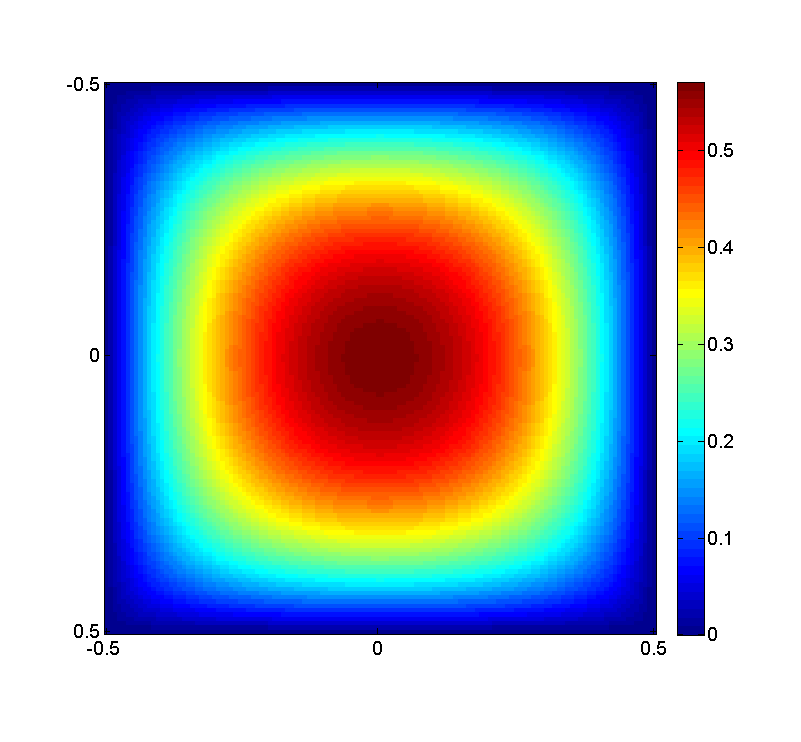
\includegraphics[width=0.6\textwidth]{img/sq_vx}
%  \label{fig:sq_vx}
%  \caption{截面速度}
%\end{figure}
    %\end{minipage}
  %}
  %\\
  %\subfigure[$y=0$处速度分布]{
    %\begin{minipage}[b]{0.6\textwidth}
\begin{figure}[htb]
  \centering
  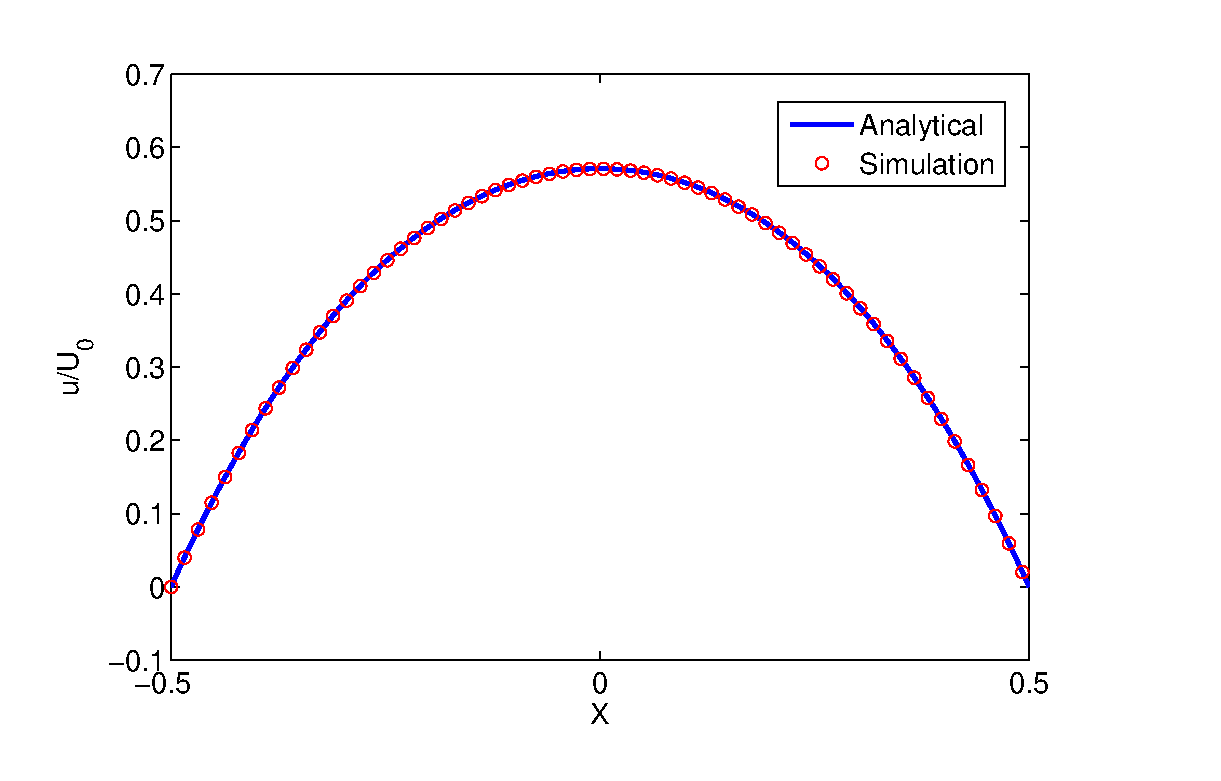
\includegraphics[width=0.7\textwidth]{img/sq_u}
  \caption{截面上$y=0$处速度与解析解比较}
   \label{fig:sq_vx}
    %\end{minipage}
  %}
\end{figure}
%\subsection{圆柱绕流}
%\subsection{简单二维多空介质流动}
GPU程序中由于采用了4.1节中指出的方法,可以不用另外执行\textbf{LBExchange} Kernel,
因为流出Block的PDF又流回到了Block的另一侧,这正好符合周期性边界实现方式。
固壁边界需要另外的Kernel来进行非平衡外推处理。 我们对不同Block尺寸和不同网格规模
下的计算速度做了测试,结果如图\ref{fig:sq_speed}所示。作为对比,CPU程序在不同网格规模
下的计算均为$4\sim5$MLUPS左右。可见我们实现的GPU程序最快可以加速两个量级以上。
\begin{figure}[htb]
  \centering
  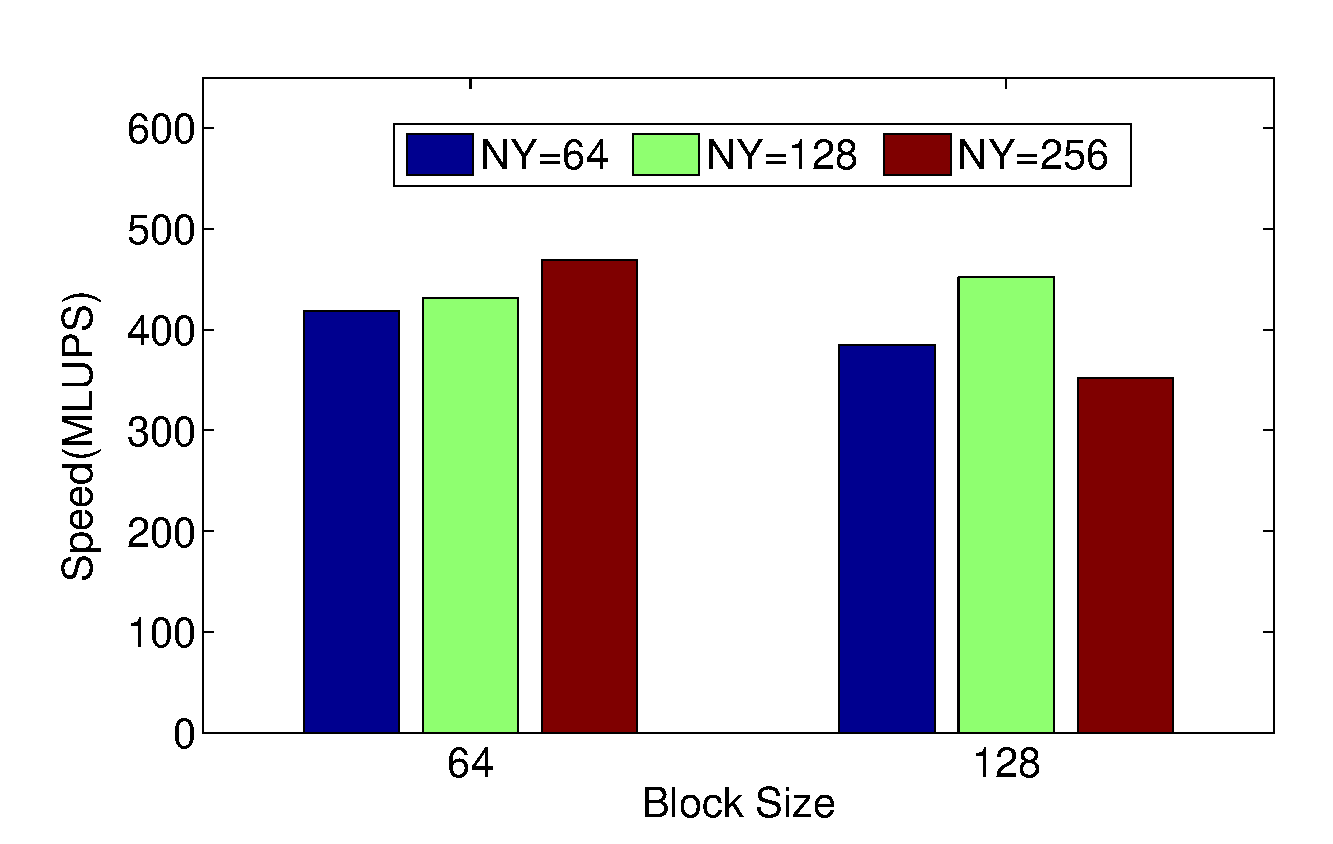
\includegraphics[width=0.6\textwidth]{img/sq_speed}
  \caption{不同Block尺寸和网格规模下的计算速度}
  \label{fig:sq_speed}
\end{figure}

\section{小结}
本章首先介绍了LBM在GPU上实现的基本方法及优化策略,然后利用按照这些方法
实现的GPU程序模拟了二维方腔流和三维方形截面直管道流。模拟结果均与解析解
或参考文献吻合良好,证明GPU程序正确的实现了LBM算法。
之后又测试了GPU程序性能,并考察了影响计算速度的因素。两个算例的GPU程序
的计算速度均为CPU版本的两个量级以上。下一章,我们将考虑流固边界较为复杂的
渗流问题。



%%%%%%%%%%%%%%%%%%%%%%%%%%%%%%%%%%%%%%%%%%%%%%%%%%%%%%%%%%%%%%%%%%%%%%%%%%%%%%%%%%%%
% Singel Phase
\chapter{单相渗流LB模拟在GPU上的实现及优化}
上一章中计算所使用的算例流场边界都比较规则、简单,流场内部格点都是
流体格点,每个格点执行的操作都相同,线程中几乎没有逻辑判断分支语句。
这在GPU实现时意味着同一个Wrap中的各个线程执行路径完全相同,SP执行效率
最高,因此用LBM模拟这种简单流场流动时能充分发挥GPU的并行效率。但在模拟
实际问题时,流场结构通常并不规则,甚至非常复杂,如多孔介质。如何在GPU
上高效地实现这中复杂边界LBM模拟依然是当前的一个研究热点。
本章正是围绕这一问题探讨了从算法上考虑的各种优化途径,并以一个实际
多空介质流动(渗流)算例验证了优化效果。

\section{对于多孔介质的一般处理方法}
在多孔介质结构中,流体在相互连通的孔隙中流动,孔隙壁面是非规则的
固体表面。将多孔介质在空间上离散后,计算区域被划分为流体格点和固体格
点,如图\ref{fig:porous_2d}所示为二维多孔介质离散后的格点分布,图中黑色
格点表示固体,白色格子表示孔隙(流体)。在程序实现时用一个整型数组\verb+flag[NY][NX]+
来记录格点的类型,\verb+flag[y][x] = 0+表时格点\verb+(y,x)+为流体格点,等于
1则为固体格点,演化时通过这个数组判断格点类型,若为固体格点,则不作任何
处理。流固边界边界通常采用简单的标准反弹格式,处理时也需要判断周围格点类型。
\begin{figure}[htb]
  \centering
  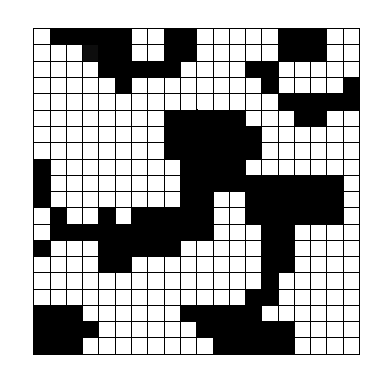
\includegraphics[width=0.6\textwidth]{img/porous_2d}
  \caption{二维多空介质示例}
  \label{fig:porous_2d}
\end{figure}

上述处理方式虽然实现起来简单,但在GPU上实现时效率不会很高。原因有二,
其一,处理每个格点时要周围格点类型,需要从全局内存加载周围格点
flag数据,占用了显存带宽,并且访存时存在第四章中所述显存地址
不对齐的情况;其二,确定周围格点类型时会引入判断分支
语句,如果一个wrap中的线程对应的格点既有流体格点,又有固体格点,
则会导致该wrap中的线程串行执行,执行效率将大为降低,在均匀的各向
同性介质中,这种情况将尤为明显,因为几乎每个wrap中都产生了分支。
上述方式除了在GPU上执行效率不高外,还存在另一个问题\--- 浪费存储
空间,因为在开辟PDF(速度分布函数)数组时,不参与计算的固体格点也占据了存储空间。
并且多孔介质的孔隙率越低,无效格点所占比例越高,存储空间浪费越严重。

%针对上述两个,我们分别采用两个方法解决
针对前一个问题,我们采用\textit{位存储模式}结合\textit{逻辑运算}方式解决,
针对第二个问题,我们采\textit{稀疏存储模式}解决。

另外,考虑到本文
最终目的是要做多组分模拟,我们在这里并没有采用第四章中所描述的使用共享内存
进行辅助迁移的方法,而是在碰撞之前从周围格点直接读取PDF。
之所以这样做,是因为在多组分模拟时,每个格点需要迁移的PDF几乎翻倍,
如果还是用共享内存辅助迁移,则SM的利用率会因共享内存数量限制而降低,进而
影响程序性能。Obrecht等人对这两种执行迁移步骤的方法做了详细对比,并指出
第二种方法在模拟复杂问题如非等温情况时,会比第一种方法效率更高\ucite{obrecht2011new}。

\section{优化技术一 ~ 位存储和逻辑运算} \label{sec:opt1}
因为每个格点只能是流体格点或固体格点,所以理论上在flag中只用一个bit就可以反映
格点类型。为了避免在演化过程中从加载周围格点的flag位,可以事先把这些
信息存储在当前格点的flag中。按这种方法,对于DnQq模型,每个格点的flag要存储$q$bit的信息,
其中$1$bit反映该格点本身类型,另外$(q-1)$bit反映周围格点类型。对于D3Q19模型,
可以用一个\texttt{int}类型($32$bit)来表示flag,如图\ref{fig:bitmap}所示,最低位
表示当前格点本身类型,第1到18位分别表示第1到18个方向上相邻格点的类型(0或1)。
\begin{figure}[htpb]
  \centering
  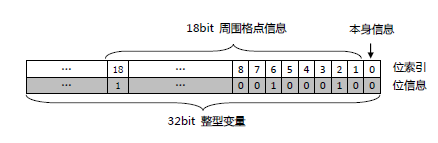
\includegraphics[]{img/bitmap}
  \caption{D3Q19模型falg的位存储模式示意}
  \label{fig:bitmap}
\end{figure}
利用这种位存储模式,解决了占用存储带宽的问题,接下来介绍利用逻辑运算来统一处理
内部流体格点和固体边界处流体格点的方法。

通常在处理流场内部格点和边界流体格点,程序会进入不同的分支语句。这里以修正反弹
格式为例,在这种反弹格式中,边界流体格点也需要执行碰撞,但它们与内部格点不同的是,
在从周围格点读取PDF时,如果该在该方向上临近格点是固体点,则从其本身的反方向读取PDF。
这里笔者提出一种能同一处理内部格点与边界格点的方法,这种方法可以保证同一个wrap中
各个线程执行的指令完全相同,指令吞吐量最高。代码\ref{code:opt2}示例了如何使用逻辑运算实现这种
方法。

\begin{Code}
\begin{lstlisting}
  ...
  //由于程序中使用了动态内存存储PDF
  //`所以用`GID`宏来做数组索引转换`
  //(z, y, x)格点(当前点)在一维数组中的位置
  k = GID(z,y,x); 
  flag_k = flag_h[k]; //当前点的flag
  //当前点为流体格点时才进行下面处理
  if(!(flag_k & 1)) 
  {
    ...
    for(i=1;i<Q;i++)  //读取各个方向上前一格点的PDF
    {
      //是否从本身读取PDF
      readShift = (flag_k & (1<<i)) == 0; 
      //`读取`PDF`的方向`
      i_reverse = i + (readShift^1)*((i&1)*2 - 1);
      xp = x - readShift*e[i_reverse][0];   
      yp = y - readShift*e[i_reverse][1];
      zp = z - readShift*e[i_reverse][2];
      kp = GID(zp, yp, xp);  
      //正式加载PDF
      F[i] = fIn[i_reverse*size + kp]; 
      ...
    }
  }
\end{lstlisting}  
\caption{优化技术一}
\label{code:opt2}
\end{Code}
如果周围格点时流体点则\texttt{readShift=1},表示读取位置有偏移,否则从自己读,
\texttt{readShift=0},没有偏移。如果读取位置有偏移,则从\texttt{i}方向的反
方向(\texttt{i\_reverse}读(此时\texttt{i\_reverse != i})。
因为我们在定义离散速度方向时,保持了第\texttt{i}个与第\texttt{i+1}个方向正好
相反(\texttt{i}为偶数),所以可以通过\texttt{i}的奇偶性判断其反方向。

值得注意的是上述优话指令流的方法也可以运用于其他需要避免\texttt{if}语句的地方,具有一定的
通用性。

\section{优化技术二 ~ 稀疏存储模式}\label{sec:opt2}
稀疏存储模式是指只存储流体格点PDF,目的是为了节省内存或显存(GPU程序),通常
GPU显存并不大(几GByte),因此在GPU程序中,这一方法更为重要。稀疏存储模式中,
首先遍历\texttt{flag}数组,统计出流体格点个数,然后动态分配一维线性内存/显存
存储流体格点PDF,流体格点的PDF按格点在遍历过程中出现的顺序插入该线性内存,如图\ref{fig:node_map}。
由于流体格点分布不规则,所以流体格点之间的相对位置关系丢失了,在迁移时不能确定
周围格点PDF的内存/显存地址。解决这个问题的办法是引入一个辅助数组来保存每个
格点各个方向上相邻格点在的位置,我们称这个数组为\texttt{node\_map}。在GPU上
实现时,\texttt{node\_map}按\texttt{node\_map[Q-1][num\_F]}形式存储数据,即依然
保证访问地址连续。
%流体格点之间的相对位置关系,
\begin{figure}[htpb]
  \centering
  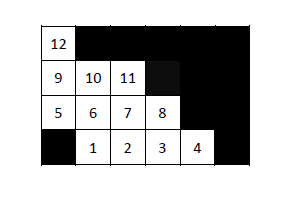
\includegraphics[]{img/node_map}
  \caption{稀疏存储模式}
  \label{fig:node_map}
\end{figure}
稀疏模式还有一个附加优点,因为在\texttt{node\_map}中直接存储了
\emph{每个周围格点的PDF}在PDF数组中的索引,这样可以在构造\texttt{node\_map}时
将反弹格点与周期边界格点的迁移源地址或目的地址地直接存在里面,
而在演化过程中不需要显示处理这些特殊格点,因而
Kernel函数大为简化。

引入辅助数组之后,虽然每个格点要存储的信息增多了,但在孔隙率低于某个阈值(
当PDF采用双精度时,该阈值约为为0.7)时
总的内存/显存用量仍低于全存储模式\ucite{pan2004high}。

值得指出的是,稀疏存储模式在CPU上和GPU上运用都可以节省存储空间,但在CPU
上相对于全存储模式并不会提高计算速度,而在GPU上却可以显著提高。这是
GPU和CPU构架差异造成的,当在GPU上运用全存储模式时,不参与计算的无效格点
占据了SP执行时间,而采用稀疏存储模式时,则不存在这一问题。本章后面
分析GPU程序性能将会验证这个现象。
%ADD 确定内存用量

\section{算例一 ~ BCC结构渗透率的测定}
\subsection{问题描述}
单相流体在外力或压差驱动下流过多孔介质时,其平均流速(达西速度)可由
达西定律给出
\begin{equation}
  u_d = -\frac{k}{\rho \nu}(\nabla p_z + \rho g)
  \label{darcy}
\end{equation}
其中$k$为多孔介质的渗透率,其具体值只有多孔介质结构本身确定,与其中
所通过的流体性质无关。本算例中使用的多孔介质模型BCC结构的渗透率具有
近似解析解,我们将其与数值模拟得出的渗透率对比来验证程序正确性。

BCC结构是指体心立方结构(Body Centered Cubic),它是一种理想多空介质
模型,其结构如图\ref{fig:bcc_array}所示,其中球体表示固体区域。因为球体
排布具有空间周期性,所以计算区域只取其一个基本单元,如图\ref{fig:bcc}所示,
其二维投影如图\ref{fig:bcc_2d}。
\begin{figure}[htpb]
  \centering
  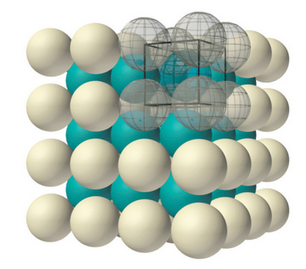
\includegraphics[]{img/bcc_array}
  \caption{BCC结构示意图}
  \label{fig:bcc_array}
\end{figure}

\begin{figure}[htb]
  \centering
  \subfigure[BCC结构基本单元]{
    \begin{minipage}[b]{0.4\textwidth}
      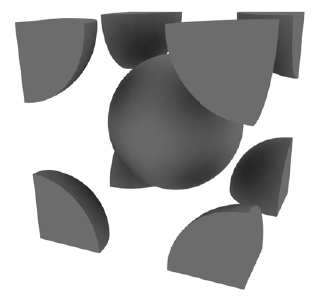
\includegraphics[width=1\textwidth]{img/bcc}
      \label{fig:bcc}
    \end{minipage}
  }
  \subfigure[BCC结构二维投影]{
    \begin{minipage}[b]{0.4\textwidth}
      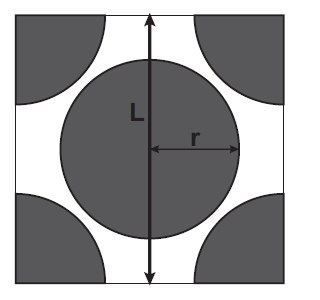
\includegraphics[width=1\textwidth]{img/bcc_2d}
      \label{fig:bcc_2d}
    \end{minipage}
  }
  \caption{BCC结构及参数}
\end{figure}
BCC结构参数为球体半径$r$和立方体单元边长$L$。固体区域所占体积比例与孔隙率分别是
\begin{equation}
  c=\frac{8\pi r^3}{L^3}, \quad \epsilon = 1-c
  \label{bcc_c}
\end{equation}
其中$c$的最大值为$c_{max} = \frac{\sqrt{3}\pi}{8}$,通常用一个取值范围为0到1的
无量纲形状因子$\chi = \left(\frac{c}{c_{max}}\right)^{1/3}$来表示球体填充的致密程度,$\chi=1$时填充
最为致密的情况,图\ref{fig:bcc}就是这种情况。
BCC结构的绝对渗透率近似解析解形式为
\begin{equation}
  k = \frac{2\epsilon r^2}{9d^*(1-\epsilon)}
  \label{k_ana}
\end{equation}
其中$d^*$是单个球体所受流体拖拽力的无量纲阻力,在$Re<1$的情况下其级数近似
解析解\ucite{sangani1982slow}为
\begin{equation}
  d^* = \sum\limits_{n=0}^{30}\alpha_n\chi^n
  \label{d_star}
\end{equation}
其中多项式系数$\alpha_n$为常数,具体值见参考文献\cite{sangani1982slow}。

\subsection{数值方法}
我们通过给定外力$g$,在流场稳定后测出达西速度$u_d$,然后根据式\eqref{darcy}得出
渗透率数值解。流场的所有外边界均为周期性边界,流固边界采用修正反弹格式,外力离散格式
采用Luo的二阶矩模型\ucite{luo1998unified}。模拟过程中保证$Re < 1$,网格规模均为$128^3$,
立方体尺寸为128m。计算收敛标准为计算所得渗透率相邻1000步的相对变化小于$10^{-5}$。如
无特别指明,所有工况在GPU上均用单精度计算。

Pan等人指出用LBGK模型计算多空介质介质流动时,
存在计算所得渗透率时与粘性相关的非物理现象,
而MRT模型可以显著改善这一问题\ucite{pan2006evaluation}。
这里我们也采用D3Q19 LBGK 和D3Q19 MRT模型并验证了这一现象。在程序实现时我们分别采用
了前两节所介绍的优化技术。

\subsection{计算结果}
%由于采用不同算法只影响计算结果而不影响计算结果,所以这里
\subsubsection{MRT与LBGK}
我们分别用LBGK和MRT模型计算了不同孔隙率和不同流体粘性对应的绝对渗透率。图\ref{fig:bcc_streamline}
和图\ref{fig:bcc_U}所示为$\chi = 0.8,\tau=0.8$时用LBGK计算得到的
流线图和沿外力方向的速度分布图。
\begin{figure}[htb]
  \centering
  \subfigure[流线图]{
    \begin{minipage}[b]{0.4\textwidth}
      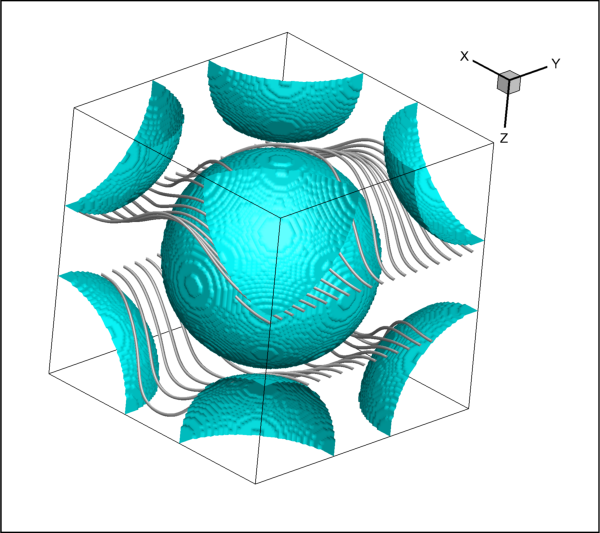
\includegraphics[width=1\textwidth]{img/bcc_streamline}
      \label{fig:bcc_streamline}
    \end{minipage}
  }
  \subfigure[沿外力方向的速度分量]{
    \begin{minipage}[b]{0.4\textwidth}
      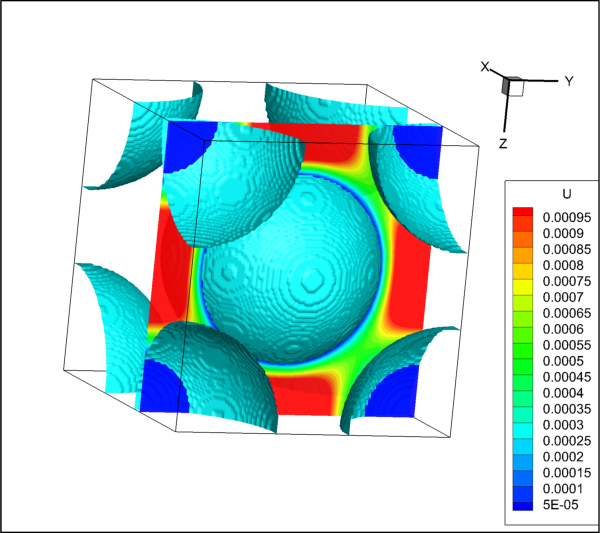
\includegraphics[width=1\textwidth]{img/bcc_U}
      \label{fig:bcc_U}
    \end{minipage}
  }
  \caption{LBGK模型$\chi=0.8, \tau=0.8$计算结果}
\end{figure}

\begin{figure}[htb]
  \centering
  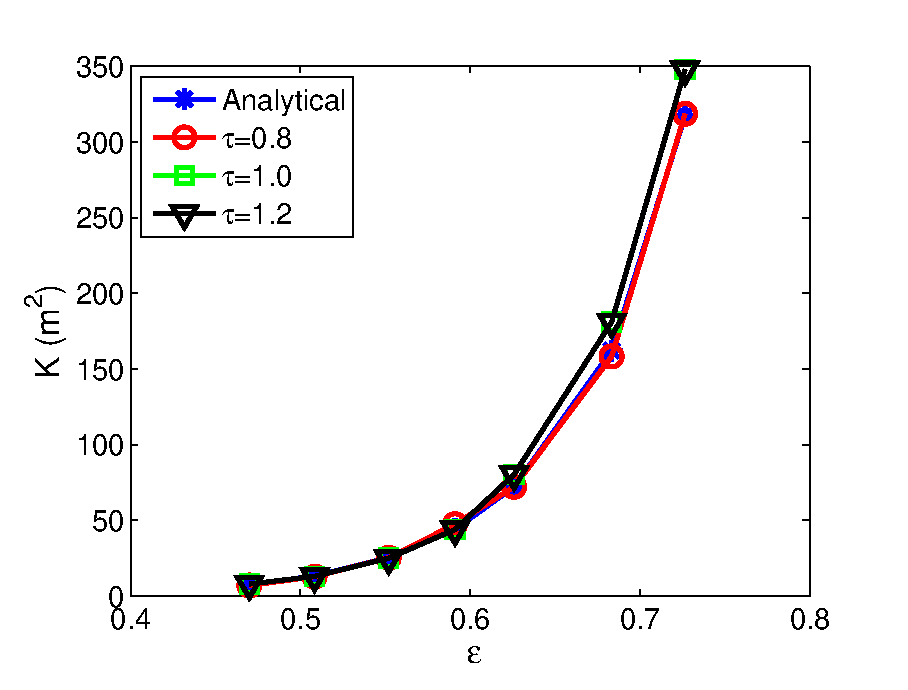
\includegraphics[width=0.6\textwidth]{img/k_bgk}
  \caption{使用LBGK模型时不同粘性和孔隙率下渗透率数值解}
  \label{fig:suckbgk}
\end{figure}

\begin{figure}[htb]
  \centering
  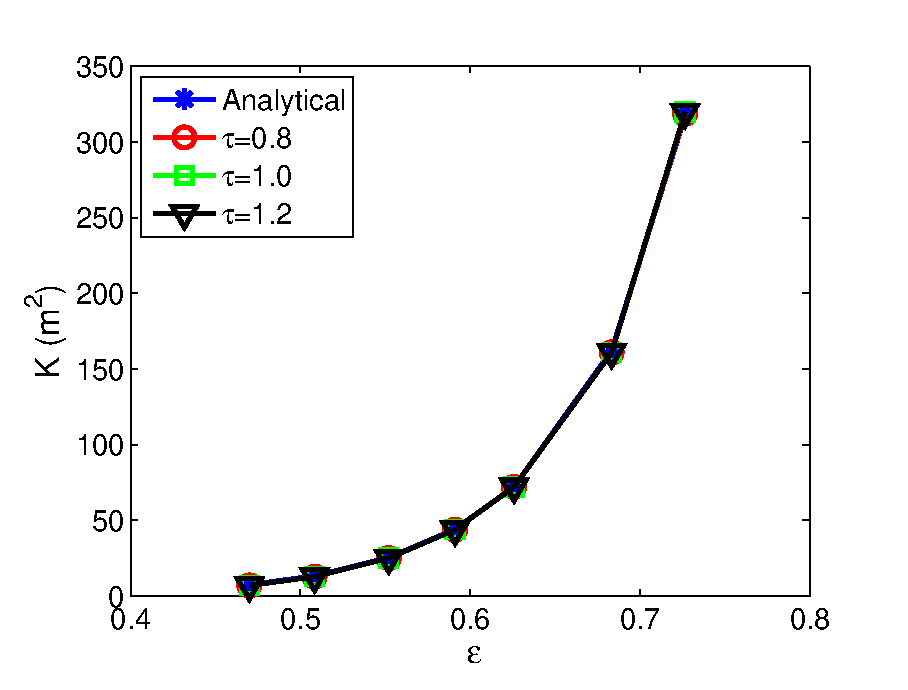
\includegraphics[width=0.6\textwidth]{img/k_mrt}
  \caption{使用MRT模型时不同粘性和孔隙率下渗透率数值解}
  \label{fig:suckmrt}
\end{figure}

图\ref{fig:suckbgk}和图\ref{fig:suckmrt}分别为不同孔隙率和不同流体粘性时计算得出的渗透率,
可以看出使用LBGK模型计算出来的渗透率会随粘性不同而变化明显,尤其是在孔隙率较高时,
而使用MRT模型计算出来的渗透率与粘性几乎无关。我们的计算得到的渗透率与解析解吻合良好,
并成功验证了文献\cite{pan2006evaluation}的结论,这证明我们的程序的实现方法正确。

\subsubsection{计算精度的影响}
在目前的GPU构架上,通常在单精度计算要比双精度计算快得多
(见3.2节),但单精度数只有7位有效数字,
相比较而言双精度数有16位有效数字。对于大多数工程应用计算
单精度已经足够,但对计算要求十分精确的场合必须使用双精度。
本小节考察本节算例中单精度和双精度对计算结果的影响。

我们分别使用单精度和双精度计算了上小节中$\chi = 0.6, \tau=1.2$的工况,
所用程序为MRT程序。
我们比较了用两种精度计算时渗透率$k$的收敛过程,其结果如图\ref{fig:dp_sp}所示。
可以明显发现二者有一定区别,
单精度计算演化39000步之后收敛,收敛值为$315.45$,而双精度计算
演化24000步就已经收敛,收敛值为$319.74$。单精度相对双精度相差$1.34\%$,
%这一差值在工程计算单精度计算
这说明单精度计算只能要求不太高的工程问题计算。

\begin{figure}[htb]
  \centering
  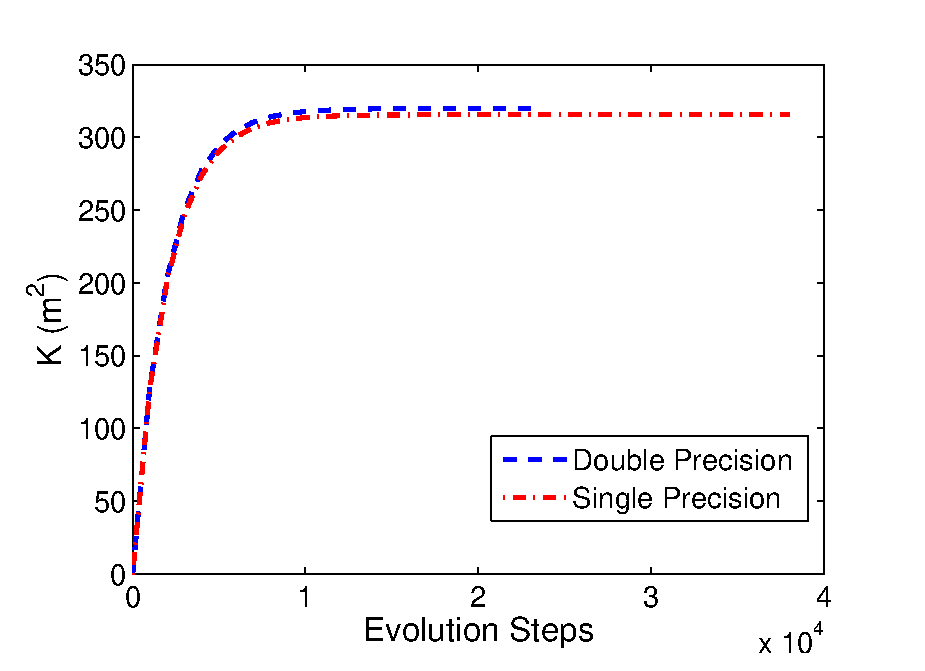
\includegraphics[width=0.6\textwidth]{img/dp_sp}
  \caption{使用单精度和双精度计算时渗透率$k$的收敛过程}
  \label{fig:dp_sp}
\end{figure}

%我们比较了二者在演化30000步之后,垂直
%于外力方向的中心截面上$\bm X$方向的速度分量(该截面位置如图\ref{fig:bcc_U}所示)。
%二者相对差别按下式计算
%\begin{equation}
  %\delta u_r =  \frac{\sqrt {\sum\nolimits_{ij}{| \bm u_{ij}^{dp}- \bm u_{ij}^{sp} |^2}}}{\sqrt{\sum\nolimits_{ij}{|  \bm u_{ij}^{dp} |^2}}}
  %\label{diff_dp_sp}
%\end{equation}
%式中上标$sp$和$dp$分别表示单精度和双精度。

\subsection{计算速度分析}
在这一小节中,我们分析各种影响计算速度的因素,包括所使用的优化算法(见5.2、5.3节)、
模型(MRT和LBGK)、计算精度、Block尺寸。在下面的比较中,如无特别指明,均采用单精度计算,Block尺寸
为64。另外,我们在4.2节中指出衡量多孔介质模拟计算速度时有两种单位\--- MLUPS
和MFLUPS,后者只统计流体格点更新,即考虑了孔隙率对计算量的影响,二者换算关系为
\begin{equation}
  Speed\text{(MFLUPS)} = \epsilon \times Speed \text{(MLUPS)}
  \label{speed_relation}
\end{equation}
在本小节的图中,我们会明确标出所使用的衡量单位。为叙述方便我们在后文中称5.2节中
中算法为算法一,而称采用5.3节中介绍的稀疏存储模式的算法为算法二。

为方便对比,我们还编写了同样计算这个问题的CPU版本程序,采用intel icc编译器编译,并加上了
\texttt{-fast}编译选项(这是目前我们所能利用的最快的编译方法),
在各种工况下观测到的最高流体格点更新速率为3.61MFLUPS。

\subsubsection{算法的影响}
图\ref{fig:speed_algo_ML}所示为采用两种算法在不同孔隙率下的计算速度,单位为MLUPS,
图\ref{fig:speed_algo_MFL}反映相同内容,不过单位为MFLUPS。
\begin{figure}[htb]
  \centering
  \subfigure[衡量单位:MLUPS:]{
    \begin{minipage}[b]{0.42\textwidth}
      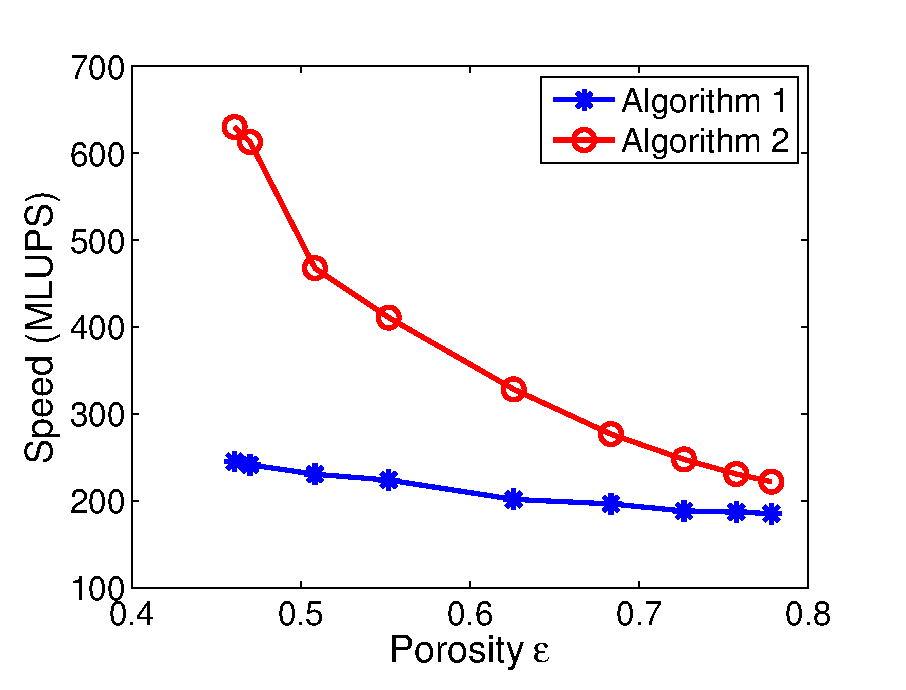
\includegraphics[width=1\textwidth]{img/speed_algo_ML}
      \label{fig:speed_algo_ML}
    \end{minipage}
  }
  %\hspace{2em}
  \subfigure[衡量单位:MFLUPS]{
    \begin{minipage}[b]{0.42\textwidth}
      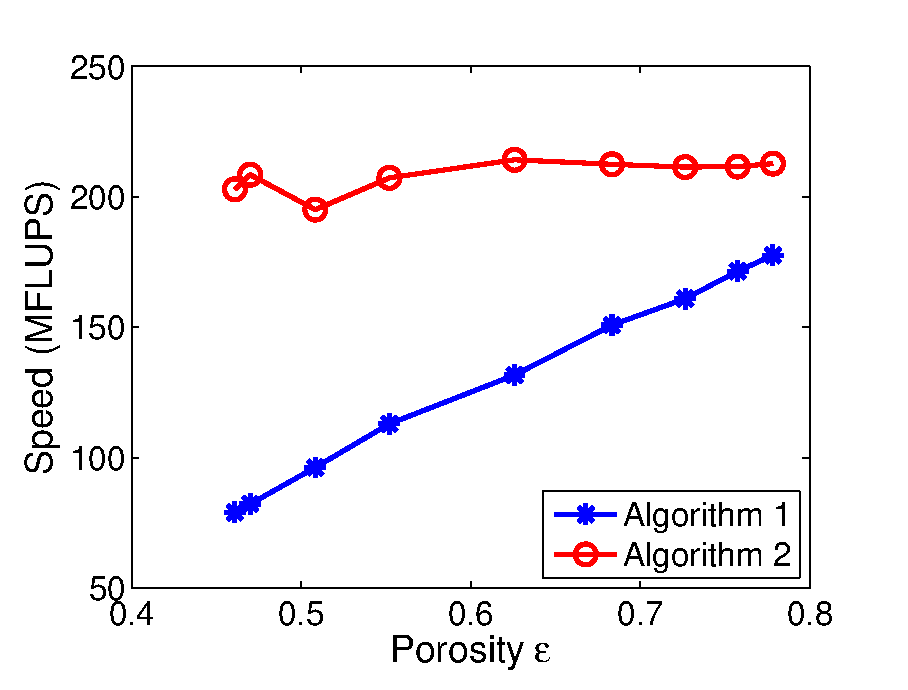
\includegraphics[width=1\textwidth]{img/speed_algo_MFL}
      \label{fig:speed_algo_MFL}
    \end{minipage}
  }
  \caption{算法对计算速度的影响}
\end{figure}
对比图\ref{fig:speed_algo_ML}中的红线和蓝线可以发现,随着孔隙率减小,采用算法二
格点更新速度大幅提高,而采用算法一则速度只有很小的提高,并且在所考差的孔隙率范围
内算法二格点计算速度均优于算法一。对比\ref{fig:speed_algo_ML}中的红线和蓝线可以发现,
随着孔隙率减小,算法一的流体格点更新速度几乎线性减小而算法二则没有显著变化,我们分析
这是因为采用算法一时,同一个wrap中的每个无效格点(固体)虽然不参与计算,但也
占据了SP执行时间。

\subsubsection{MRT和LBGK模型的影响}
MRT模型相对于BGK模型只在计算量上有所增加,而访存模式即访存大小都没有变化。通常
文献中反映其计算量约增加了$15\%\sim20\%$\ucite{guoredbook}。这里我们分析了
采用算法一时两者的计算速度的差别,其结果见图\ref{fig:speed_model},图中所示
为在不同孔隙率下采用MRT模型计算速度相对LBGK模型的下降量,可以发现相对下降量
都小于10\%。
\begin{figure}[htb]
  \centering
  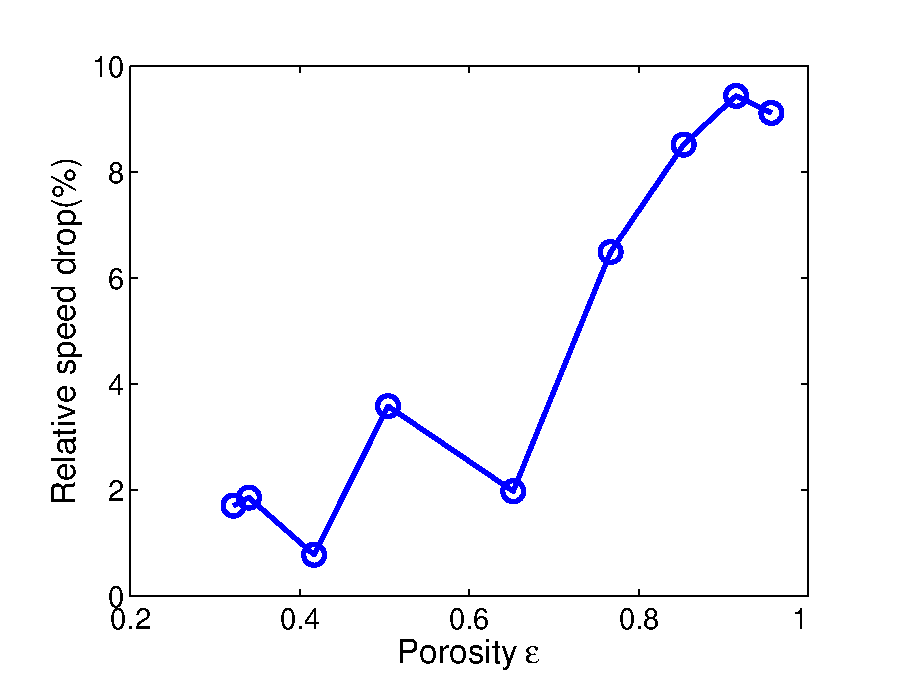
\includegraphics[width=0.6\textwidth]{img/speed_model}
  \caption{MRT模型相对LBGK模型计算速度的相对下降量}
  \label{fig:speed_model}
\end{figure}

\subsubsection{单、双精度的影响}
我们采用算法一结合MRT模型比较了单、双精度的计算速度,结果如图\ref{fig:speed_dpsp}所示,
可以发现双精度计算速度为单精度的34\%左右。在我们所使用的Tesla C1060 GPU上,双精度计算
速度理论上是单精度的$1/12$,而此处34\%与之相差较大,我们分析这是因为LB的计算性能瓶颈在
显存带宽而不在处理器执行速度,双精度计算相对单精度带宽需求只增大一倍,考虑到其他因素
如访存效率影响,此处43\%在预期范围内。
\begin{figure}[htb]
  \centering
  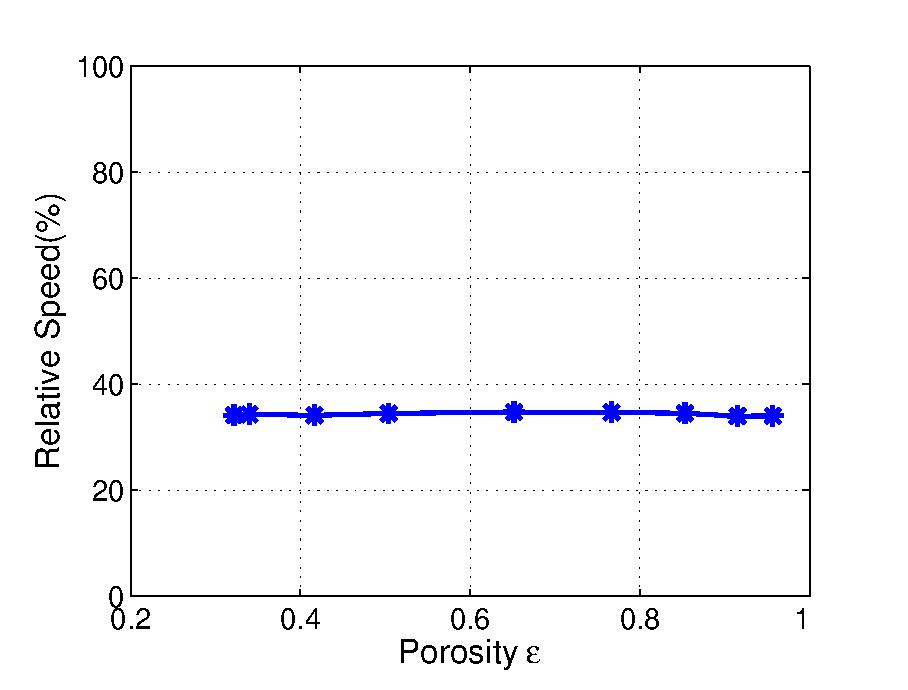
\includegraphics[width=0.6\textwidth]{img/speed_dpsp}
  \caption{双精度相对单精度的计算速度}
  \label{fig:speed_dpsp}
\end{figure}

\subsubsection{Block尺寸的影响}
上面的速度测试Block大小都是64, 这里我们分别测试了Block大小为96和128时的计算速度。
采用的的模型和算法分别是MRT模型与算法二。
结果见图\ref{fig:speed_block},可以发现Block大小为64时速度最高,而为96和128时
速度较小且差别不大,这是定型的计算效率受到寄存器或共享内存数量限制的现象。
考虑到我们Kernel只使用了寄存器,而没有使用共享内存,所以此处Block尺寸增大时,性能
下降的现象应该是性能受到寄存器数量的限制引起的。
\begin{figure}[htb]
  \centering
  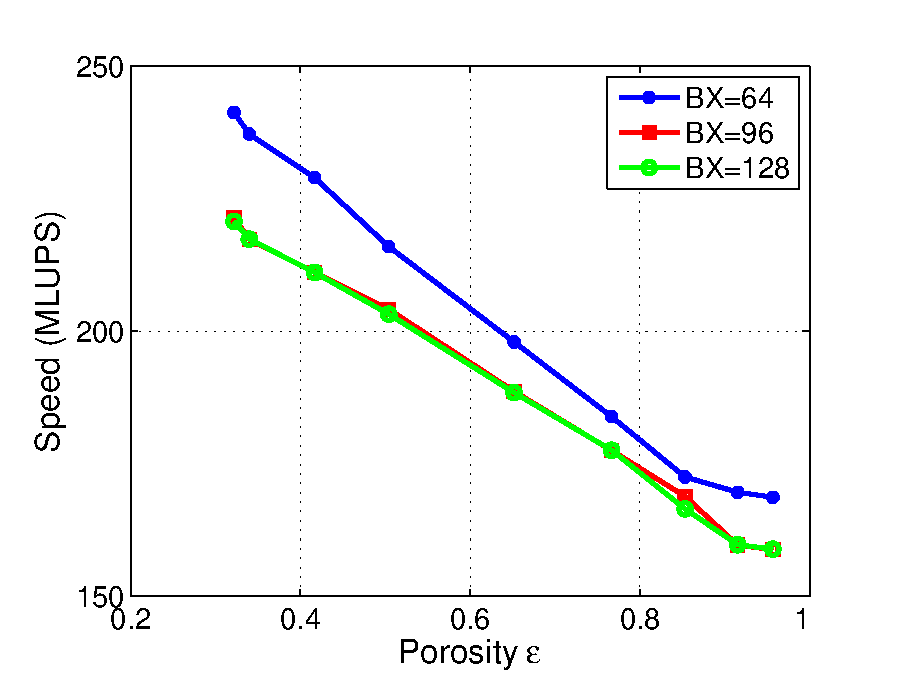
\includegraphics[width=0.6\textwidth]{img/speed_block}
  \caption{不同Block大小时的计算速度}
  \label{fig:speed_block}
\end{figure}

\section{小结}
本章中我们首先介绍了LBM处理多孔介质的一般方法,
并指出了两种针对在GPU上实现多孔介质流动模拟的优化技术
\---利用位操作结合逻辑运算减小访存量和优化指令流以及利用稀疏存储模式减小
显存用量和提高程序计算速度。
随后我们分别运用这两个优化技术编制了LBGK模型和MRT模型的GPU程序计算了BCC
多孔介质模型的渗透率,与解析解对比发现吻合良好,证明了我们GPU程序实现
正确。最后我们详细分析了上述GPU程序的计算速度,详细考察了各种影响计算
速度的因素,在最优情况,我们的GPU程序计算速度可达212MFLUPS和630MLUPS。
超过CPU串行程序50倍。在下一章中我们将本章介绍的优化算法运用于更复杂的多孔介质内的多相流LBM
模拟。


%%%%%%%%%%%%%%%%%%%%%%%%%%%%%%%%%%%%%%%%%%%%%%%%%%%%%%%%%%%%%%%%%%%%%%%%%%%%%%%%%%%%
% Multi-Phase
\chapter{多相渗流模拟在GPU上的实现}
多孔介质内的多相流动是一类常见的复杂流动现象,在化石能源开采,化工过程,新能源等应用广泛。
目前LBM是模拟这类流动现象流行的数值方法,这得益于LBM在处理复杂流固边界和刻画多相多组分之间
相互作用的独特优势(见第\ref{chp:LBM}章)。但与上一章介绍的多孔介质内单相流动一样,在孔隙尺度
下直接运用LBM模拟多相渗流计算量通常相当大,一般需要利用并行计算加速。利用GPU加速LBM孔隙尺度
多相流计算目前在文献中报道较少,这也是本文工作的一个重点。
%ADD 前人在这方面工作相对较少。
本章讨论基于2.4节中多组分/多相模型的GPU实现。我们用两个算例验证了
多相流GPU程序实现的正确性,随后用其该模拟了二维和三维多孔介质中的两相流动,最后测试了其计算速度。
%ADD  上面的工作是否能完成

%%%%%%%%%%%%%%%%%%%%%%%%%%%%%%%%%%%%%%%%%%
\section{两组分LBM的GPU实现}
%多组分LBM与单组份LBM的GPU实现上有一些差异。
两组分LB模时,每个格点同时有两套PDF在演化,并且要考虑两组分间的相互作用对PDF变化的贡献。
就数据访问模式而言,每个格点除访问本身和周围格点的PDF外,还要访问其宏观量。在单组份情况
各个格点计算平衡态时只需要知道其本身的宏观量,即具有最理想的空间局部性,所以其计算过程
可以融合在计算迁移的Kernel中,也不需要为宏观量开辟存储空间,
但在两组分情况时,每个格点要访问周围格点的宏观量,若在碰撞迁移的Kernel中计算相邻格点的
宏观量显然进行大量的重复计算,因此我们采取的策略是为每个组分的宏观量$\rho_k$、$\bm u_k$
开辟全局内存,并另外增加一个Kernel\---\texttt{LBUpdateMacros},它在碰撞迁移的Kernel执行
完后统计每个组分的宏观量。

%%%%%%%%%%%%%%%%%%%%%%%%%%%%%%%%%%%%%%%%%%
\section{程序验证}
%%%%%%%%%%%%%%%%%%%%%%%%%%
\subsection{静止气泡测试} \label{subsec:bubble}
静止气泡测试可验证Laplace定律,是两相流中标准的模型验证算例之一。
Laplace定律给出了两相界面间压差$\Delta p$和界面表面张力$\gamma$之间的关系
\begin{equation}
  \Delta p = \sigma\frac{\gamma}{r}
  \label{laplace}
\end{equation}
对于二维情况$\sigma=1$,三维情况$\sigma=2$。对于球形界面$r$为球体半径,对于
圆柱形界面$r$为圆柱半径。

在进行静止气泡测试时,在计算区域中心球形区域内放置一种组分(即所谓的“气泡”),
球形区域以外放置另一种组分,待流场稳定后,压力场和气泡半径不再变化,如图\ref{fig:bubble}
所示。初始化流场时放置不同半径的气泡,稳定后得到不同的气泡半径$r_i$和界面压差$\Delta p_i$。
按照Laplace定律,$\Delta p_i$和$1/r_i$应该成正比。

这里指出,虽然我们编制的是D3Q19的GPU程序,但是为减少计算量,在实际计算时,
X方向只有一层格点,并且是周期边界,相当于计算的二维情况,后面的几个算例也是这种情况。

初始化时一个圆形状的组分被放在在YZ平面中心,平面四边均为周期边界,如图\ref{fig:bubble}所示。
%\begin{figure}[htb]
  %\centering
  %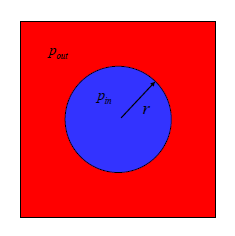
\includegraphics[]{img/bubble}
  %\caption{气泡示意图}
  %\label{fig:bubble}
%\end{figure}

\begin{figure}[htb]
  \centering
  \begin{tikzpicture}
    \draw[fill=blue!20] (-2,-2) rectangle (2,2);
    \draw[fill=red!70] (0,0) circle (1);
    \draw (-0.3,-0.3) node[]{$P_{in}$};
    \draw (-1.2,1.2) node[]{$P_{out}$};
    \draw[->] (0,0) -- (0.707, 0.707) node[pos=0.5,sloped, above]{$r$};
  \end{tikzpicture}
  \caption{气泡示意图}
  \label{fig:bubble}
\end{figure}

%\begin{figure}[htb]
  %\centering
  %\subfigure[气泡示意图]{
    %\begin{minipage}[b]{0.4\textwidth}
      %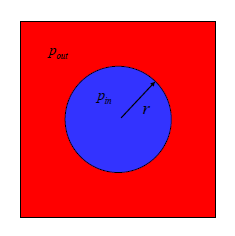
\includegraphics[width=1\textwidth]{img/bubble}
      %\label{fig:bubble}
    %\end{minipage}
  %}
  %\subfigure[测试结果]{
    %\begin{minipage}[b]{0.4\textwidth}
      %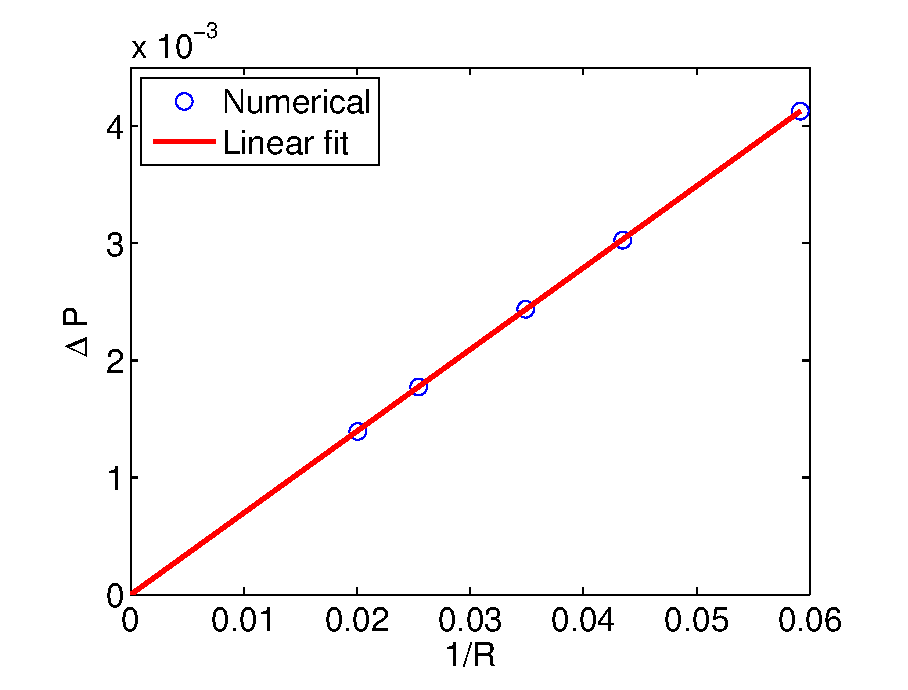
\includegraphics[width=1\textwidth]{img/bubble_test}
      %\label{fig:bubble_test}
    %\end{minipage}
  %}
  %\caption{气泡测试}
%\end{figure}

测试时两种流体粘性都为$1/6$,密度都为$1$,XY平面格点数为$128\times128$,
组分间相互作用系数$g_{k\bar k}=0.2$。
测试结果如图\ref{fig:bubble_test},可以看出计算结果与Laplace定律吻合良好。
\begin{figure}[htb]
  \centering
  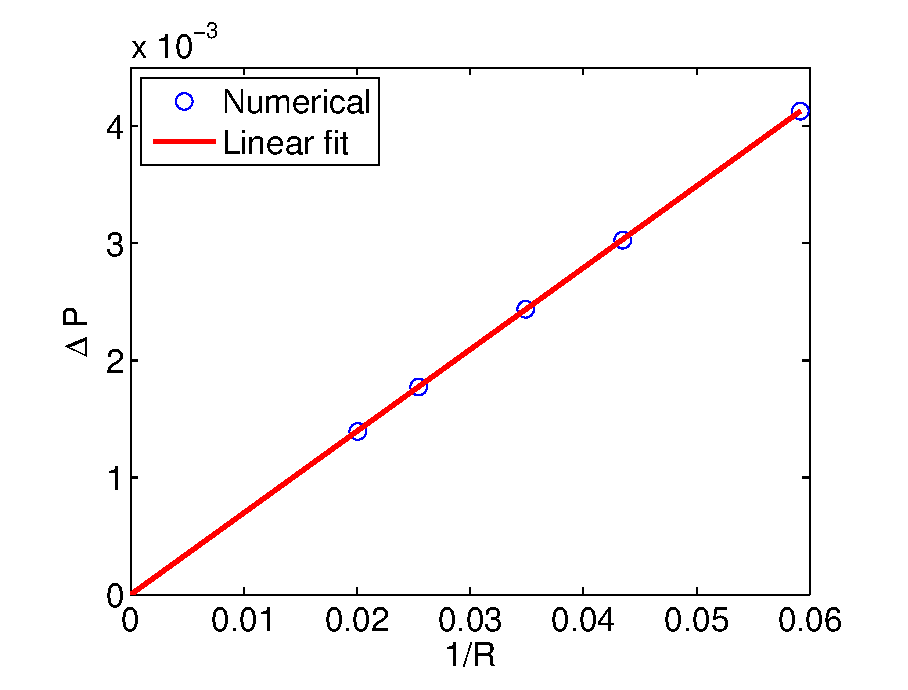
\includegraphics[width=0.6\textwidth]{img/bubble_test}
  \caption{气泡测试}
  \label{fig:bubble_test}
\end{figure}

%%%%%%%%%%%%%%%%%%%%%%%%%%
\subsection{层状两相流}
层状两相流如图\ref{fig:lcf}所示,在两块水平放置的平板间,两相流体在
沿X方向的外力驱动下一起向前运动。其中非润湿相处于中间层,厚度为$2a$,
而润湿相则贴近板壁,两板相距$2L$。两相流体受到的外力可以不同,分别为
$F_w$和$F_n$,下标$n$和$w$表示润湿相(wetting phase)和非润湿相(no wetting
phase)。
两相流体X方向速度在沿Y方向分布的解析解为\ucite{porter2012multicomponent}
\begin{subequations}\label{lcf_ana}
  \begin{flalign}
    u(y)=\frac{F_n}{2\nu_n\rho_n}(a^2-y^2)+\frac{F_w}{2\nu_w\rho_w}(L^2-a^2),
    \quad 0\leqslant |y|\leqslant a \\
    u(y)=\frac{F_w}{2\nu_w\rho_w}(L^2-y^2), \quad a \leqslant |y| \leqslant L
  \end{flalign}
\end{subequations}
\begin{figure}[htb]
  \centering
  \begin{tikzpicture}[scale = 1.5]
    \draw[fill=blue!20] (-3,-1) rectangle (3,1);
    \draw[dashed, fill=red!70] (-3,-0.5) rectangle (3,0.5);
    \draw[very thick](-3, 1) -- (3,1);
    \draw[very thick](-3, -1) -- (3,-1);

    \draw[dashed, thick](-3.2, 0) -- (3.2,0);

    \draw (-2,0.75) node[] { 润湿相};
    \draw (-2,-0.25) node[] {非润湿相};

    \draw[->, thick] (0, 0.75) node[left] {$\bm  F_w$} -- (0.5, 0.75);
    \draw[->, thick] (0, -0.25) node[left] {$\bm  F_n$} -- (0.5, -0.25);
    \draw[->] (-2.5, 1.3) node[left]{平板} -- (-2, 1.05);
    \draw[<->] (2.6, 0) -- node[left]{$a$}  (2.6, 0.5);

    \draw (3, 1) -- (3.15, 1);
    \draw[<->] (3.1, 0) -- node[right]{$L$}  (3.1, 1.0);
  \end{tikzpicture}
  
  \caption{层状两相流示意图}
  \label{fig:lcf}
\end{figure}

%\begin{figure}[htb]
  %\centering
  %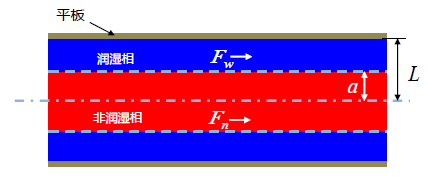
\includegraphics[]{img/lcf}
  %\caption{层状两相流示意图}
  %\label{fig:lcf}
%\end{figure}

算例中设置的计算参数为$\rho_n=\rho_w=1.0$,$\nu_w=10/6,\nu_n=1/6$,
$F_n=F_w=1.0\time10^{-6}$,组分间作用系数$g_{k\bar k}=0.27$,Y方向
网格个数为256。计算结果与解析解的对比如图\ref{fig:lcf_vx_a}所示,可以
发现二者吻合良好。
\begin{figure}[htb]
  \centering
  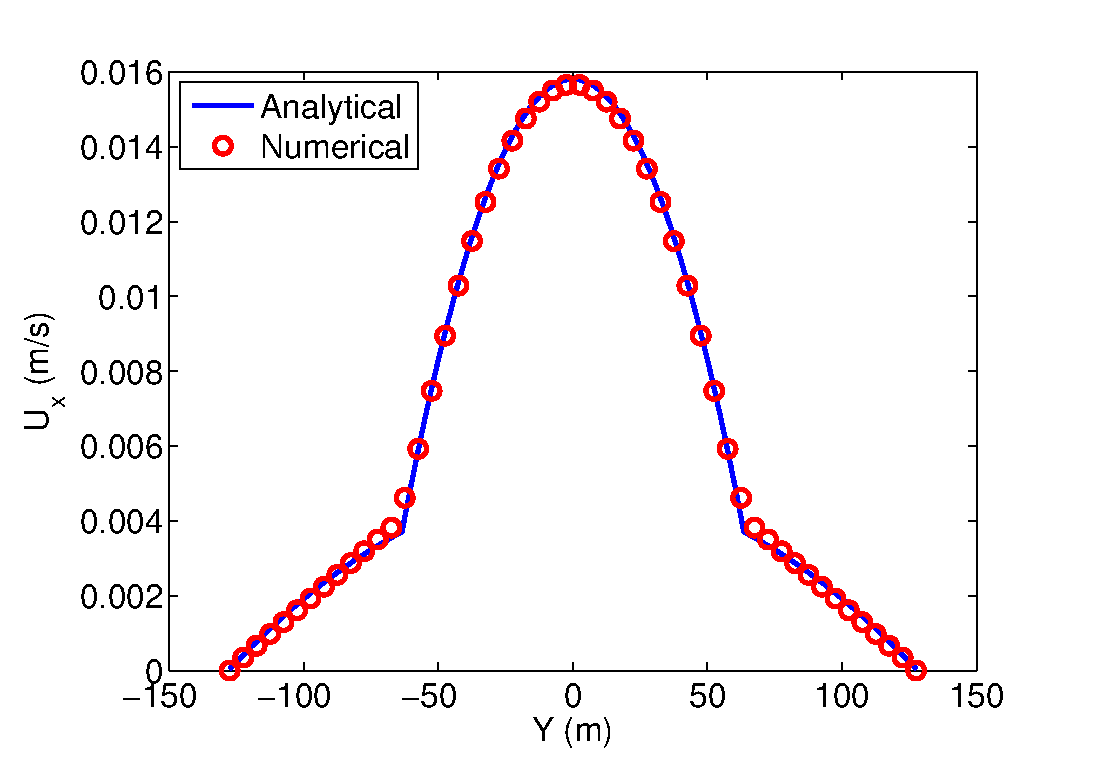
\includegraphics[width=0.6\textwidth]{img/lcf_vx_a}
  \caption{沿Y方向的速度分布}
  \label{fig:lcf_vx_a}
\end{figure}

%%%%%%%%%%%%%%%%%%%%%%%%%%
\subsection{液滴测试}
为验证润湿性边界条件处理的正确性,我们进行了液滴测试,并获得了组分
固体表面间相互作用强度与接触角的关系。组分与固体表面的接触角反应了两种
组分对固体表面的相对润湿性。在Shan-Chen模型(或我们所使用的改进模型)
中,接触角大小主要取决于两种流体组分(组分g与f)与固体表面(s)
间相互作用强度系数$G_{gs}$、$G_{gs}$以及组分间相互作用强度系数$G_{fg}$。
另外,$G_{fg}$大小影响相界面厚度和数值稳定性,我们发现$G_{fg}=0.2$时比较
理想,所以接下来的测试中取$G_{fg}=0.2$。

计算开始时,在一个长$800$高$200$的二维长管道的下底板放置一个半径为$50$半圆形组分
f,其他区域分布着另一组分g,管道左右边界是周期边界,上下边界是固壁,
示意图见图\ref{fig:droplet}。
%\begin{figure}[htb]
  %\centering
  %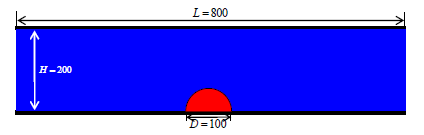
\includegraphics[]{img/droplet}
  %\caption{液滴示意图}
  %\label{fig:droplet}
%\end{figure}

\begin{figure}[htb]
  \centering
   \begin{tikzpicture}[scale = 1.5]
    \draw[fill=blue!20] (-4, 0) rectangle (4,2);
    \draw[<->] (-3.5, 0) -- node[right]{$H=200$} (-3.5, 2);
    \draw[very thick] (-4, 2) -- (4, 2);
    \draw[very thick] (-4, 0) -- (4, 0);
    \draw[|<->|] (-4, 2.1) -- node[above]{$L=800$} (4, 2.1);
    %\draw[fill=red!50] (0:0.5) -- arc (0:180:0.5);
    \draw[thick, fill=red!50] (0:0.6) arc (0:180:0.6);
  \end{tikzpicture}
  \caption{液滴示意图}
  \label{fig:droplet}
\end{figure}
通过调整$G_{fs}$、$G_{gs}$的取值,液滴会呈现不同接触角,计算结果见图
\ref{fig:drop_A}至图\ref{fig:drop_G}。
每幅图只画出了液滴附近的区域。

\begin{figure}[htb]
  \centering
  \subfigure[$G_{fs}=-0.005, G_{gs}=0.005$]{
    \begin{minipage}[b]{0.4\textwidth}
      
\includegraphics[width=0.8\textwidth]{img/drop_img/drop_A}
      \label{fig:drop_A}
    \end{minipage}
  }
  \subfigure[$G_{fs}=0.0, G_{gs}=0.0$]{
    \begin{minipage}[b]{0.4\textwidth}
      
\includegraphics[width=0.8\textwidth]{img/drop_img/drop_E}
      \label{fig:drop_E}
    \end{minipage}
  }
  \\
  \subfigure[$G_{fs}=-0.01, G_{gs}=0.01$]{
    \begin{minipage}[b]{0.4\textwidth}
      
\includegraphics[width=0.8\textwidth]{img/drop_img/drop_B}
      \label{fig:drop_B}
    \end{minipage}
  }
  \subfigure[$G_{fs}=0.01, G_{gs}=-0.01$]{
    \begin{minipage}[b]{0.4\textwidth}
      
\includegraphics[width=0.8\textwidth]{img/drop_img/drop_F}
      \label{fig:drop_F}
    \end{minipage}
  }
  \\
  \subfigure[$G_{fs}=-0.02, G_{gs}=0.02$]{
    \begin{minipage}[b]{0.4\textwidth}
      
\includegraphics[width=0.8\textwidth]{img/drop_img/drop_C}
      \label{fig:drop_C}
    \end{minipage}
  }
  \subfigure[$G_{fs}=0.02, G_{gs}=-0.02$]{
    \begin{minipage}[b]{0.4\textwidth}
      
\includegraphics[width=0.8\textwidth]{img/drop_img/drop_G}
      \label{fig:drop_G}
    \end{minipage}
  }
  \\
  \subfigure[$G_{fs}=-0.03, G_{gs}=0.03$]{
    \begin{minipage}[b]{0.4\textwidth}
      
\includegraphics[width=0.8\textwidth]{img/drop_img/drop_D}
      \label{fig:drop_D}
    \end{minipage}
  }
  \subfigure[$G_{fs}=0.03, G_{gs}=-0.03$]{
    \begin{minipage}[b]{0.4\textwidth}
      
\includegraphics[width=0.8\textwidth]{img/drop_img/drop_H}
      \label{fig:drop_H}
    \end{minipage}
  }
  \caption{接触角测试结果}
\end{figure}

%%%%%%%%%%%%%%%%%%%%%%%%%%%%%%%%%%%%%%%%%%
\section{多相渗流模拟}
在上一节中的验证算例中,流固边界相对简单,我们在这一节中
计算了实际多孔介质中的二维和三维两相渗流。
%%%%%%%%%%%%%%%%%%%%%%%%%%%%%%%%%%
\subsection{二维多相渗流模拟}
计算过程使用的二维多孔介质如图\ref{fig:porousMedid2D}所示,
图中黑色区域为固体,白色部分为孔隙,前处理时将其离散为$802\times478$
的个格子大小。初始化时,在孔隙中随机布满两种纯组分,即每个孔隙格点
以相同的概率被设为组分f或g。两种组分粘性为$\nu_f=\nu_g=1/6$,密度
为$\rho_f=\rho_g=1$。流体在向右的大小为$F=10^{-4}$的外力驱动下运动。
组分间相互作用强度为$G_{gf}=0.15$, 组分与固壁间的相互作用强度分别为
$G_{fs}=0.03,G_{gs}=-0.03$,根据上一节液滴测试的结果,在这组参数下,
组分f形成的相是非润湿相,而组分g形成的相是润湿相,并且非润湿相
接触角接近$180^o$。
%布满两种流体组分$f$和$g$,
\begin{figure}[htb]
  \centering
  
\includegraphics[width=0.6\textwidth]{img/porousMedia2D}
  \caption{二维多孔介质结构}
  \label{fig:porousMedid2D}
\end{figure}
图\ref{fig:porousMedid2D_A}至\ref{fig:porousMedid2D_E}所示为不同演化步
时两相的分布,其中红色部分为润湿相(组分g),蓝色部分为非润湿相(组分f)。
可以发现在流动过程中润湿相包围着固壁,而非润湿相则被润湿相包围,这是
多相渗流基本的现象。
\begin{figure}[htb]
  \centering
  \subfigure[第1000步]{
    \begin{minipage}[b]{0.4\textwidth}
      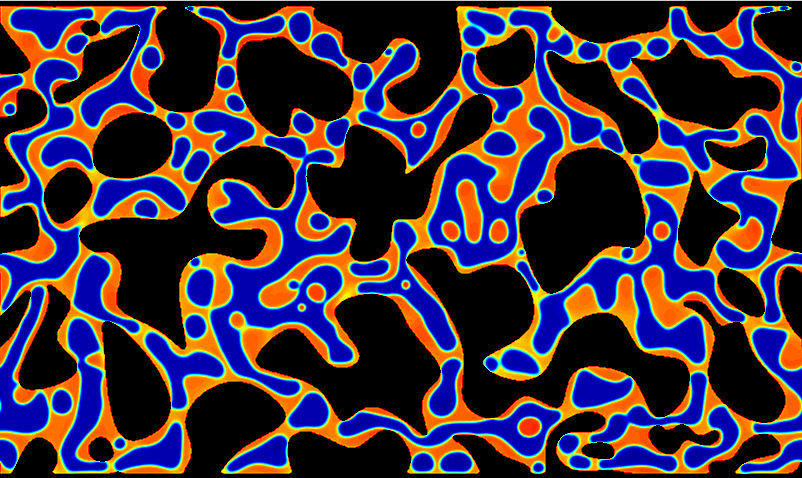
\includegraphics[width=0.8\textwidth]{img/open/GG_00001000}
      \label{fig:porousMedid2D_A}
    \end{minipage}
  }
  \subfigure[第5000步]{
    \begin{minipage}[b]{0.4\textwidth}
      
\includegraphics[width=0.8\textwidth]{img/open/GG_00005000}
      \label{fig:porousMedid2D_B}
    \end{minipage}
  }
  \\
  \subfigure[第10000步]{
    \begin{minipage}[b]{0.4\textwidth}
      
\includegraphics[width=0.8\textwidth]{img/open/GG_00010000}
      \label{fig:porousMedid2D_C}
    \end{minipage}
  }
  \subfigure[第20000步]{
    \begin{minipage}[b]{0.4\textwidth}
      
\includegraphics[width=0.8\textwidth]{img/open/GG_00020000}
      \label{fig:porousMedid2D_D}
    \end{minipage}
  }
  \\
  \subfigure[第30000步]{
    \begin{minipage}[b]{0.4\textwidth}
      \includegraphics[width=0.8\textwidth]{img/open/GG_00030000}
      \label{fig:porousMedid2D_E}
    \end{minipage}
  }
  \subfigure[第40000步]{
    \begin{minipage}[b]{0.4\textwidth}
      \includegraphics[width=0.8\textwidth]{img/open/GG_00040000}
      \label{fig:porousMedid2D_F}
    \end{minipage}
  }
  \caption{二维多相渗流模拟}
\end{figure}

%%%%%%%%%%%%%%%%%%%%%%%%%%%%%%%%%%

\subsection{三维维多相渗流模拟}
这一节中我们模拟了一种人工生成的多孔介质内的两相流,该多孔介质由
大小和位置随机分布的球体堆积而成,其孔隙结构如图\ref{fig:balls}所示,
其孔隙率大小为0.7。各个面均为周期性边界条件,初始化时孔隙内各格点
按相等概率随机给定组分f或组分g。流体受沿X方向的外力驱动。
演化100000步时,流场内部两相分布如图\ref{fig:3d_porous_2_phase}所示,
其中蓝色部分为固体区域,红色部分为非润湿相,绿色部分为润湿相。

\begin{figure}[htpb]
  \centering
  \subfigure[随机球体堆积多孔介质模型]{
    \begin{minipage}[b]{0.4\textwidth}
      \includegraphics[width=0.9\textwidth]{img/3d_porous/balls}
      \label{fig:balls}
    \end{minipage}
  }
  \subfigure[演化100000步时两相分布]{
    \begin{minipage}[b]{0.4\textwidth}
      \includegraphics[width = 0.9\textwidth]{img/3d_porous/2_phase}
      \label{fig:3d_porous_2_phase}
    \end{minipage}
  }
  \caption{三维多孔介质两相流}
\end{figure}


\section{性能测试}
\subsection{性能测试}
\subsubsection{性能预测}
%多相流计算程序相对于单相流计算程序在算
我们根据上一章中单组分流动稀疏存储算法GPU程序性能来预测本章多组分模拟GPU程序性能,二者在计算上的区别有如下几点:
\begin{itemize}
  \item 两组分程序中每个格点存储两套PDF,并且碰撞前需要访问相邻格点宏观量,访存量增加
    超过1倍;
  \item 两组分程序碰撞前需要计算组分间相互作用,计算量增大;
  \item 两组分程序中多了一个\texttt{LBUpdateMacros} Kernel函数;
  \item 两组分程序需特殊处理流固边界(润湿性边界),引入线程判断和分支;
\end{itemize}
考虑到LB的GPU计算性能瓶颈在访存带宽,所以上述几个因素中第一个因素对性能影响最大,即两组分相对单组份性能至少下降
一半。
另外我们运用CUDA工具箱中的Visual Profiler 分析发现\texttt{LBUpdateMacros} Kernel函数占整个演化过程计算时间的22\%左右。
综合上述因素我们预测两组分相对单组份计算速度下降70\%左右。上一章中采用稀疏存储算法的单组分计算GPU程序的流体格点更新速率为
210MFLUPS左右(单精度,见图\ref{fig:speed_algo_MFL}),因此我们预测本章的两组分计算程序速度大概为60MLUPS。

\subsubsection{网格数的影响}
我们分别测试了二维和三维流场在不同网格数下的计算速度,流场中不含固体格点(即Kernel中没有判断分支),二维和
三维计算采用的是同一个程序,二维情况只算一层流体格点(见\ref{subsec:bubble}小节解释)。采用单精度计算时,
速度测试结果如图\ref{fig:chp6_speed_2d}和\ref{fig:chp6_speed_3d}所示。
可以发现二维和三维情况计算速度均为70MLUPS左右,三维情况最高速度可达80MLUPS。
\begin{figure}[htpb]
  \centering
  \subfigure[二维]{
    \begin{minipage}[b]{0.4\textwidth}
      \includegraphics[width=0.9\textwidth]{img/chp6_speed_2d}
      \label{fig:chp6_speed_2d}
    \end{minipage}
  }
  \subfigure[三维]{
    \begin{minipage}[b]{0.4\textwidth}
      \includegraphics[width=0.9\textwidth]{img/chp6_speed_3d}
      \label{fig:chp6_speed_3d}
    \end{minipage}
  }
  \caption{网格数对计算速度的影响}
\end{figure}

\subsubsection{流固边界的影响}
因为Kernel函数中处理流固边界润湿性时引入了分支判断语句,对GPU程序执行效率会有影响。
我们测试在不同复杂程度的流场时的计算速度,所用三种流场如图\ref{fig:chp6_A}至\ref{fig:chp6_C}所示。
图\ref{fig:chp6_A}为最简单的情形,没有固体格点;图\ref{fig:chp6_B}所示为上一节中使用的随机球体
多孔介质模型,其流场较为复杂;图\ref{fig:chp6_C}为随机生成的方块填充多孔介质结构,其流场
结构最为复杂。
\begin{figure}[htpb]
  \centering
  \subfigure[没有固体格点]{
    \begin{minipage}[b]{0.3\textwidth}
      \includegraphics[width=0.9\textwidth]{img/3d_porous/A}
      \label{fig:chp6_A}
    \end{minipage}
  }
  \subfigure[随机球体]{
    \begin{minipage}[b]{0.3\textwidth}
      \includegraphics[width=0.9\textwidth]{img/3d_porous/B}
      \label{fig:chp6_B}
    \end{minipage}
  }
  \subfigure[随机方块]{
    \begin{minipage}[b]{0.3\textwidth}
      \includegraphics[width=0.9\textwidth]{img/3d_porous/C}
      \label{fig:chp6_C}
    \end{minipage}
  }
  \caption{不同复杂程度的流场结构}
\end{figure}

三种情况网格数均为$64\times 64 \times 128$,速度测试结果如图\ref{fig:chp6_speed_ABC}所示。
可以发现流场结构越复杂,计算速度越慢,最复杂的情况相对最简单的情况计算速度下降33\%。
\begin{figure}[htb]
  \centering
  \includegraphics[width=0.6\textwidth]{img/chp6_speed_ABC}
  \caption{流场复杂程度对计算速度的影响}
  \label{fig:chp6_speed_ABC}
\end{figure}

%\subsection{程序结构}
%本节简介本本研究过程中针对多孔介质中单相/多相流所开发的GPU计算程序。

%根据前面章节介绍的系数存储模式,首先要根据表示多孔介质结构的\texttt{flag}数组
%重构格点的之间的连接关系。我们将这一过程与计算过程分开处理,作为前处理过程。

\section{小结}
本章介绍了两相渗流LB模拟在GPU上的实现。
针对多组分LB模型在GPU上实现时的难点我们重新设计了演化的Kernel函数,
并增加了一个Kernel单独计算宏观量。
我们首先通过气泡测试、层状两相流、接触角测试验证了我们程序实现的正确性,
随后分别模拟了二维和三维的两相渗流,计算结果显示的流动现象与实际情况相符。
最后进行了程序性能测试,并分析了影响计算速度的因素,发现我们的两组分GPU程序
的最高计算速度可达80MFLUPS,而我们计算相同问题的CPU版本程序速度最快为1.96MFLUPS,
因此GPU加速比超过40。



%%%%%%%%%%%%%%%%%%%%%%%%%%%%%%%%%%%%%%%%%%%%%%%%%%%%%%%%%%%%%%%%%%%%%%%%%%%%%%%%%%%%
\chapter{全文总结}
本文主要研究了复杂边界流动的格子Boltzmann模拟在GPU上的高性能并行实现。

我们首先按文献中常见的运用共享内存进行辅助迁移的方法
实现了针对简单流动的LBM算法GPU程序,并用其
模拟了二维顶盖驱动方腔流和三维外力驱动方截面直管道流。
在验证了程序正确性后我们测试了其计算速度。我们发现
在简单流场情况下,利用该方法可以达到相对于CPU程序
两个量级的加速比。

考虑到GPU搭载的共享内存十分有限,在实现多组分LBM模型的时候
共享内存大小容易成为性能瓶颈,我们在接下来实现的程序中并没有
采用前面利用共享内存辅助迁移的方案,
而是探究了其他优化方法,其一为利用位操作结合逻辑运算减少访存量
并优化指令流,其二为利用稀疏存储模式大幅降低模拟多孔介质流动时
的计算量。我们分别基于这两种优化方法编制了相应的GPU程序计算
一种理想多孔介质模型(BCC结构)的绝对渗透率,计算结果与解析解
吻合良好,随后测试了两种优化方法的效果,发现第二种算法具有较大
优势,能大幅减少显存耗用和计算量,尤其是在多孔介质孔隙率较低的情况下。

%目前模拟多孔介质内多组分多相流动的LBM
本文另外一个工作是针对我们所使用的多组分LBM模型计算特点,
提出了该模型在GPU上的高效实现方法,并基于这个方法开发了具有一定通用性的GPU并行计算程序。
在利用该程序其模拟了基本的多相问题,验证了其正确性之后,我们用它模拟了真实多孔介质中的多相渗流。
最后,我们还对其进行了性能测试和分析。

本研究工作还有一些问题值得进一步研究,如目前的计算程序只使用了单GPU计算,
实际进行大规模三维并行LBM模拟时,
单个GPU提供的显存空间有限,必须结合使用多线程技术或OPENMP/MPI并行利用多个GPU并行计算才能满足
存储空间要求。另外我们实现的GPU程序的通用性有待进一步提高,如实现不同如入口边界条件的设置等等。
笔者将在今后的工作中着手解决这些问题。

% Conclusion

%%%%%%%%%%%%%%%%%%%%%%%%%%%%%%%%%%%%%%%%%%%%%%%%%%%%%%%%%%%%%%%%%%%%%%%%%%%%%%%%%%%%
%% 致谢
%%%%%%%%%%%%%%%%%%%%%%%%%%%%%%%%%%%%%%%%%%%%%%%%%%%%%%%%%%%%%%%%%%%%%%%%%
%
%   LaTeX File for Doctor (Master) Thesis of Tsinghua University
%   LaTeX + CJK     清华大学博士(硕士)论文模板
%   Based on Wang Tianshu's Template for XJTU
%   Version: 1.00
%   Last Update: 2003-09-12
%
%%%%%%%%%%%%%%%%%%%%%%%%%%%%%%%%%%%%%%%%%%%%%%%%%%%%%%%%%%%%%%%%%%%%%%%%%
%   Copyright 2002-2003  by  Lei Wang (BaconChina)       (bcpub@sina.com)
%%%%%%%%%%%%%%%%%%%%%%%%%%%%%%%%%%%%%%%%%%%%%%%%%%%%%%%%%%%%%%%%%%%%%%%%%


%%%%%%%%%%%%%%%%%%%%%%%%%%%%%%%%%%%%%%%%%%%%%%%%%%%%%%%%%%%%%%%%%%%%%%%%%
%
%   LaTeX File for phd thesis of xi'an Jiao Tong University
%
%%%%%%%%%%%%%%%%%%%%%%%%%%%%%%%%%%%%%%%%%%%%%%%%%%%%%%%%%%%%%%%%%%%%%%%%%
%   Copyright 2002  by  Wang Tianshu    (tswang@asia.com)
%%%%%%%%%%%%%%%%%%%%%%%%%%%%%%%%%%%%%%%%%%%%%%%%%%%%%%%%%%%%%%%%%%%%%%%%%
\renewcommand{\baselinestretch}{1.5}
\fontsize{12pt}{13pt}\selectfont

\chapter*{致~~~~谢}
\markboth{致谢}{致谢}
\addcontentsline{toc}{chapter}{\hei 致谢}

本文的研究工作是在导师煤燃烧国家重点实验室郭照立教授的悉心指导下完成的。
郭老师学识渊博,是LB领域的知名学者,
他为人爽朗,治学严谨,对学生和工作极为认真负责,让本人受益匪浅。
每周的例会上,郭老师的点拨总能让我找到方向,消除困惑。
除了每周例会,在毕业设计过程中遇到困难时,郭老师总是及时跟我交流,给我指导,让我的毕业设计工作得以顺利完成。
郭老师的很多话我都记忆犹新,在以后的研究中,他的严谨作风仍会继续带给我积极的影响。在此,谨向郭老师致以最衷心的感谢。
同时还要感谢煤燃烧实验室606郭老师课题组的各位师兄师姐们,是他们营造了一个团结、积极、活跃的学术氛围。
在本论文的完成过程中,笔者曾无数次请教了课题组的娄钦和刘高洁两位博士师姐、王亮和杨康两位博士师兄另外还有
数学院的黄昌盛博士,在这里
也对他们表示衷心感谢。

最后感谢我的家人对我一如既往的关心和付出。


%参考文献
\wuhao

\bibliographystyle{unsrt}

\ifpdf \phantomsection \fi

\addcontentsline{toc}{chapter}{\hei 参考文献}

%\addtolength{\itemsep}{-0.8 em} % 缩小参考文献间的垂直间距, 在bibtex下无效
\bibliography{reference/reference.bib}
%
%\chapter*{毕业设计小结}
\markboth{毕业设计小结}{毕业设计小结}
\addcontentsline{toc}{chapter}{\hei 毕业设计小结}

这次毕业设计是对我四年本科学习的一个总结,涉及了操作系统、计算机网络、体系结构、组成原理等课程的知识,并且要求自己动手实践,这对我来说是一次全面的考验。一开始对于TinyOS和nesC语言完全是陌生的,对组件化设计的概念理解也不够深入。接着是各种安装和配置问题,只能通过官方的教程和TinyOS的邮件列表查询,信息的来源比较少。由于nesC并不是一种广泛使用的语言,因此各种相关的工具比较少,比如没有优秀的可视化工具可用,从而导致阅读TinyOS代码相对比较困难:为了找一个命令的实现,需要顺着配置文件层层挖掘,有时甚至要深入十几层才能找到具体实现的代码,后来通过自定义配置编辑器以及查找辅助工具才略微提高了一些效率,这一过程颇为坎坷。

本次毕业设计中印象比较深刻的是节点上程序的调试,节点没有足够的资源用于支持断点,甚至获知节点的当前运行状态也是相当困难的,通过串口的调试信息并不一定是实时的,因而只能通过节点上的3个LED灯得知准确状态信息,这是以后可以改进的地方。

经历了本次毕设,我对无线传感器网络有了一定的了解,积累了一些实际经验,对以后研究生阶段的学习目标也更加明确了。




%
%%  附录

%\begin{appendix}
%    \renewcommand{\chaptername}{附录\Alph{chapter}}
%   \chapter*{附~~录}
\markboth{附录}{附录}
\addcontentsline{toc}{chapter}{\hei 附录}
\noindent\bfseries\texttt{test.py}源代码:
\setmonofont{Monaco}
\lstset{basicstyle=\ttfamily\scriptsize,keywordstyle=\color{blue},commentstyle=\color{green},stringstyle=\color{red},tabsize=4,frameround=fttt,escapeinside=``,lineskip=0.6pt}
\begin{lstlisting}[language=Python]
#!/usr/bin/env python
from TOSSIM import *
from random import *
import sys

if len(sys.argv) < 3:
	print "usage: need 2 parameter, nodes number and simulate time"
	sys.exit(0)

nodes = int(sys.argv[1])
sim_time = int(sys.argv[2])
t = Tossim([])
r = t.radio()

f = open("topo.txt", "r")
lines = f.readlines()
for line in lines:
  s = line.split()
  if (len(s) > 0):
    if s[0] == "gain":
      r.add(int(s[1]), int(s[2]), float(s[3]))

noise = open("meyer-short.txt", "r")
lines = noise.readlines()
for line in lines:
  str = line.strip()
  if (str != ""):
    val = int(str)
    for i in range(0, nodes):
      m = t.getNode(i);
      m.addNoiseTraceReading(val)

for i in range(0, nodes):
  m = t.getNode(i);
  m.createNoiseModel();
  time = randint(t.ticksPerSecond(), 10 * t.ticksPerSecond())
  m.bootAtTime(time)
  print "Booting ", i, " at time ", time

print "Starting simulation."

t.addChannel("Forwarder", sys.stdout)
t.addChannel("TestNetworkC", sys.stdout)
t.addChannel("TreeRouting", sys.stdout)
t.addChannel("LI", sys.stdout)

while (t.time() < sim_time):
  t.runNextEvent()

print "Completed simulation."
\end{lstlisting}

\noindent\bfseries\texttt{ctpsim-3d.py}源代码:
\begin{lstlisting}[language=Python,tabsize=2]
#!/usr/bin/env python
import xmlrpclib,time
import re

nodes = 10
server = xmlrpclib.Server('http://localhost:20738/RPC2')
G = server.ubigraph

G.clear()

node = [0 for col in range(nodes)]

for i in range(0,nodes):
	node[i] = G.new_vertex()
	G.set_vertex_attribute(node[i], 'label', str(i))
	G.set_vertex_attribute(node[i], 'shape','sphere')
	G.set_vertex_attribute(node[i], 'size','0.5')
	G.set_vertex_attribute(node[i], 'color','#1E90FF')

edge = [[0 for col in range(nodes)] for row in range(nodes)]

for i in range(0,nodes):
	for j in range(i+1, nodes):
		edge[i][j] = G.new_edge(node[i], node[j])
		edge[j][i] = edge[i][j]

topo = open('topo.txt', 'r')
lines = topo.readlines()
for line in lines:
	s = line.split()
	if s[0] == 'gain':
		if int(s[1]) < nodes and int(s[2]) < 
				nodes and int(s[1]) < int(s[2]):
			G.set_edge_attribute(edge[int(s[1])][int(s[2])],
					     'strength',
					     str(1 + float(s[3]) / 120.0))
			#G.set_edge_attribute(edge[int(s[1])][int(s[2])],
					      'label', s[3]) # add gain value

G.set_vertex_attribute(node[0], 'color', '#FFFF00') # root node

def node_spark(node_id):
	node_id = int(node_id)
	G.set_vertex_attribute(node[node_id], 'color', '#FF0000')
	G.set_vertex_attribute(node[node_id], 'color', '#FFFFFF')
	G.set_vertex_attribute(node[node_id], 'color', '#FF0000')
	G.set_vertex_attribute(node[node_id], 'color', '#FFFFFF')
	if node_id != 0:
		G.set_vertex_attribute(node[node_id], 'color', '#1E90FF')
	else:
		G.set_vertex_attribute(node[node_id], 'color', '#FFFF00')


def node_display_debug_str(node_id, debug_str):
	G.set_vertex_attribute(node[int(node_id)], 'label', node_id+": "+debug_str)
	#time.sleep(0.0)
	#G.set_vertex_attribute(node[node_id], 'label', str(node_id))

def process_boot_at_time(node_id, time):
	G.set_vertex_attribute(node[int(node_id)], 'label','boot at:'+time)


def process_parent_change(node_id, origin_parent, new_parent):
	node_id = int(node_id)
	origin_parent = int(origin_parent)
	new_parent = int(new_parent)
	if origin_parent != 65535:
		G.set_edge_attribute(edge[node_id][origin_parent], 'color', '#C0C0C0')
		G.set_edge_attribute(edge[node_id][origin_parent], 'width','1')
	G.set_edge_attribute(edge[node_id][new_parent], 'color', '#FF00FF')
	G.set_edge_attribute(edge[node_id][new_parent], 'width','7')
	time.sleep(0.5)

def animateArrow(e, reverse):
  pos = 0.0
  if reverse:
    pos = 1.0
  G.set_edge_attribute(e, "arrow_position", str(pos))
  G.set_edge_attribute(e, "arrow_reverse", str(reverse))
  G.set_edge_attribute(e, "arrow", "true")
  for i in range(0,20):
    a = i / 19.0
    if reverse:
      a = 1.0 - a
    G.set_edge_attribute(e, "arrow_position", str(a))
    time.sleep(0.05)
  G.set_edge_attribute(e, "arrow", "false")

def animate_broadcast(node_id):
	node_id = int(node_id)
	for j in range(2):
		for i in range(21):
			G.set_vertex_attribute(node[node_id], 
				'size', str(0.5 + i / 20.0))
		for i in range(21):
			G.set_vertex_attribute(node[node_id],
				'size', str(0.5 + (20 - i)/20.0))

def process_send_beacon(node_id):
	node_id = int(node_id)
	animate_broadcast(node_id)
	

def process_forwoard_subsend(node_id, dest):
	print node_id, dest
	node_id = int(node_id)
	dest = int(dest)
	if node_id == dest:
		return
	G.set_edge_attribute(edge[node_id][dest], 'arrow','true')
	if node_id > dest:
		G.set_edge_attribute(edge[node_id][dest], "arrow_reverse", 'true')
	speed = 10 # the smaller, the faster
	for pos in range(speed+1):
			if node_id < dest:
				G.set_edge_attribute(edge[node_id][dest], 
					"arrow_position", str(pos / float(speed)))
			else:
				G.set_edge_attribute(edge[node_id][dest], 
					"arrow_position", str(1- pos / float(speed)))
			time.sleep(0.05)
	G.set_edge_attribute(edge[node_id][dest], "arrow_reverse", 'false')
	G.set_edge_attribute(edge[node_id][dest], 'arrow','false')

def dispatch_each_line(line):
	re_boot_at_time = r'Booting  (/d+)  at time  (/d+)'
	re_debug = r'^DEBUG \((\d+)\): (.*)'

	re_parent_change = r'Changed parent. from (\d+) to (\d+)'
	# 1.parent,  2.etx
	re_send_beacon = r'CtpRoutingEngineP\$0\$sendBeaconTask\$runTask parent: (\d+) etx: (\d+)' 
	# 1.dest, 2. error
	re_forward_subsend = r'CtpForwardingEngineP\$0\$SubSend\$sendDone to (\d+) and (\d+)' 

	match = re.match(re_boot_at_time, line)
	if match:
		process_boot_at_time(match.group(1), match.group(2))
	else:	# match debug messages
		match = re.match(re_debug, line)
		if match:
			node_id = match.group(1)
			node_spark(node_id)
			debug_str = match.group(2)
			node_display_debug_str(node_id, debug_str)
			
			if re.match(re_parent_change, debug_str):
				match = re.match(re_parent_change, debug_str)
				process_parent_change(node_id, match.group(1), match.group(2))
			elif re.match(re_send_beacon, debug_str):
				process_send_beacon(node_id)
			elif re.match(re_forward_subsend, debug_str):	# Forwarder send a packet
				match = re.match(re_forward_subsend, debug_str)
				process_forwoard_subsend(node_id, match.group(1))
line = raw_input()
while line:
	dispatch_each_line(line)
	line = raw_input()
\end{lstlisting}

%\end{appendix}

% 发表的文章列表

%\include{appendix/publications}

\clearpage
\end{document}

%%%%%%%%%%%%%%%%%% End of the file  %%%%%%%%%%%%%%%%%%%%%%%%
